\documentclass[12pt,oneside]{report}
\usepackage[a4paper]{geometry}
%\usepackage{showkeys}
\usepackage{listings}
\lstset{
language=C,
basicstyle=\tiny\ttfamily}

\usepackage{draftcopy}
\draftcopyName{Joao Paulo}{180}
\usepackage{joaopaulo}
\title{Apostila de Automação Industrial}
\begin{document}

\maketitle
\tableofcontents
% 

\section{Início}
Várias máquinas mecânicas de diversas graus de complexidade já foram desenvolvidas ao longo da história, como por exemplo relógios mecânicos desde o século VIII na china e desde o século XIII na Europa e os robôs de Pierre Jaquet-Droz, do século XVIII, ou ainda o mecanismo de Antikythera, datado entre 70 e 50 A.C., e que foi, aparentemente, um relógio astronômico de 27 engrenagens. Mas em termos atuais, podemos considerar o início da automação como sendo a revolução industrial. Em termos mais precisos, podemos usar, de forma levemente arbitrária, a invenção do tear mecânico por Cartwright em 1785 como sendo o ponto inicial da automação industrial. Esta invenção realiza um movimento relativamente complexo de forma automática, usando a energia obtida a partir de uma roda d'água e com a finalidade de gerar um produto (tecido) a partir de uma matéria prima (fio).
\begin{figure}
  \centering
  \includegraphics[width=\textwidth]{cartwright}
  \caption{Tear mecânico de Cartwright. Imagem retirada de...}
\end{figure}

Por volta de 1788 James Watts inventou um mecanismo de regulagem de fluxo de vapor, o que permitiu controlar a potência de caldeiras e outras máquinas a vapor, o que permite utilizar uma potência muito maior que uma roda d'água. Isto foi um grande impulso para a mecanização, com o desenvolvimento de diversos mecanismos e equipamentos. Hoje em dia chamamos isto de Indústria 1.0.

A partir da segunda metade do século XIX, houve a mudança das máquinas a vapor para máquinas a diesel e a energia elétrica. Junto a isto houve a reorganização do espaço das fábricas, fazendo as chamadas linhas de produção. Chamamos este tipo de manufatura de Indústria 2.0.

Neste período, a capacidade de automação ainda ficava muito restrita devido a dificuldade de realizar processos complexos de forma automática. Ou seja, retirava-se grande parte do esforço físico do homem, mas ainda era necessário muito esforço mental. Faltava a invenção do computador.

\begin{figure}
  \centering
  \includegraphics[width=\textwidth]{watt}
  \caption{Mecanismo de regulação de vapor de James Watt. Imagem retirada de...}
\end{figure}

\section{Computação}
Um passo na direção do desenvolvimento do computador se deu em 1820, quando o francês Charles Babbage começou a desenvolver a sua máquina diferencial, voltada para automatizar o processo mental do cálculo matemático, que hoje chamaríamos de uma calculadora mecânica. Ela evoluiu até o conceito da máquina analítica, descrita em 1837, que é considerada o primeiro projeto de computador, embora apenas partes dela tenham sido efetivamente construídas. Estima-se que se fosse totalmente construída, a máquina analítica de Babbage ocuparia um campo de futebol.
\begin{figure}
  \centering
  \includegraphics[width=\textwidth]{babbage}
  \caption{Máquina diferencial de Charles Babbage. Imagem retirada de...}
\end{figure}

Outro passo foi dado por Herman Hollerith em 1880, quando ele usou cartões perfurados como mecanismo de memória de calculadoras mecânicas. Sua intenção era a de automatizar algumas tarefas de tabulação do censo dos EUA. O uso da máquina de Hollerith fez com que o processamento dos dados do censo, que antes duravam 10 anos, fosse concluído em 6.

Em 1936, Alan Turing descreveu um \emph{computador universal} em seu artigo “On Computable Numbers, with an Application to the Entscheidungsproblem”, o que hoje é conhecido como uma \emph{Máquina de Turing}. Suas idéias foram desenvolvidas em 1944, com a construção do Colossus, considerado como o primeiro computador, embora tivesse a função específica de quebrar o código criptográfico alemão na segunda guerra. Ele consistia de um circuito com 1600 a 2400 válvulas com capacidade de processamento de vinte e cinco mil caracteres por segundo. A titulo de comparação, os computadores de uso pessoal de hoje em dia atingem 10 bilhões de cálculos por segundo, enquanto que o mais rápido computador do mundo no início de 2023 é o americano Frontier, que faz $1,194\cdot10^{18}$ cálculos por segundo (\SI{1,194}{exaflops}).

\section{Indústria 3.0}
Ao longo da primeira metade do século XX foram utilizados sistemas eletromecânicos para o controle de processos industriais, chamados circuitos chaveados. Estes sistemas utilizavam chaves e relês (chaves controladas eletricamente) para o controle lógico e para o comando de motores. Um avanço importante nesta área foi dado pelo trabalho de mestrado de Claude Shannon, em 1934, que fez a ligação entre os circuitos chaveados e a lógica matemática, permitindo o uso do ferramental lógico já existente na chamada álgebra de Boole para o projeto de circuitos ainda mais complexos. Veremos mais sobre isto no capítulo \ref{chap:CLP}.
\begin{figure}
  \centering
  \includegraphics[width=\textwidth]{circuitoChaveado}
  \caption{Exemplo de circuito chaveado. Imagem retirada de...}
\end{figure}

Na década de 60 a General Motors fez uma especificação de um equipamento que hoje chamamos de CLP -- Controlador Lógico Programável, que é justamente um computador voltado para o controle de processos industriais, o que simplifica em muito o controle de processos industriais quando comparado com a solução por circuitos chaveados. Em 1968 foi criado o primeiro e eles continuam a ser os principais equipamentos para controlar processos industriais, embora tenham obviamente evoluído muito desde esta versão inicial até os dias de hoje.
\begin{figure}
    \centering
    \includegraphics[width=\textwidth]{clp}
    \caption{Exemplo de CLP.}
\end{figure}

Junto com o CLP, nesta época houve também o desenvolvimento de outros equipamentos, tais como tornos e fresas automatizados (CNCs) e  robôs industriais. Estes equipamentos marcam a chamada Industria 3.0.

Junto com estes sistemas e equipamentos, há o uso cada vez maior de sistemas computacionais de apoio à produção, como sistemas SCADA, PIMS e outros, de controle de estoque e logística.

\section{Indústria 4.0}
O avanço da computação e da eletrônica permite o uso de equipamentos cada vez mais versáteis autônomos. O uso de redes de computadores, sensores baseados em visão computacional, automação dos sistemas de produção, entre outros, leva à Indústria 4.0, bem mais versátil que as anteriores. As redes de dispositivos, com e sem fio, e o barateamento dos sensores permite também a automação de tarefas anexas à própria manufatura, tais como a realização de manutenção preditiva, automatizando a avaliação do estado dos equipamentos utilizados.

\section{Sobre este livro}
Como se vê, a automação industrial moderna embarca muitas áreas, tais como visão computacional, robótica, logística, etc. Além dos próprios processos de manufatura específicos para cada indústria.

Mas podemos simplificar o problema da automação industrial para: fazer processos automáticos para a fabricação de produtos a partir de matérias primas e insumos com o mínimo de interferência e trabalho humano.

Para isto se requer equipamentos que que levantem o estado do processo de fabricação -- sensores -- e com base nisto atuem sobre as matérias primas -- atuadores --. A ligação entre sensores e atuadores deve seguir uma determinada lógica, o que é efetuado de modo também automático por dispositivos controladores.

Além disso, some-se que não existe, pelo menos até agora, automação que seja totalmente independente das pessoas. Logo precisa-se de sistemas supervisórios, para acompanhar o andamento do processo.

Com base nisto, este texto está separado da seguinte forma:
\begin{itemize}
    \item O capítulo \ref{chap:automacao} é mais geral. Define o que é automação industrial, descreve os tipos de automação e apresenta a pirâmide de automação.
    \item O capítulo \ref{chap:instrumentacao} apresenta vários sensores e atuadores usados em processos industriais, bem como algumas definições sobre sensores e atuadores e diagrams do tipo PI\&D.
    \item O capítulo \ref{chap:CLP} apresenta os Controladores Lógicos Programáveis, o principal tipo de controlador usado na indústria.
    \item O capítulo \ref{chap:programacao} apresenta um microcontrolador e faz a ligação entre a programação de um dispositivo como este e a programação de CLPs.
    \item O capítulo \ref{chap:ladder} explica a programação através da linguagem ladder, uma das linguagens padrões de CLPs.
    \item O capítulo \ref{chap:grafcet} detalha a linguagem gráfica grafcet e sua implementação em CLPs: Sequential Function Chart.
    \item O capítulo \ref{chap:scada} apresenta sistemas SCADA - Supervisory Control and Data Acquisition, que é o elemento mais usual para acompanhamento de um processo industrial.
    \item O capítulo \ref{chap:PIMS} sobe mais um degrau na pirâmide de automação e mostra sistemas de gerenciamento de plantas industriais, tais como o PIMS e o MES.
    \item Por último, o caítulo \ref{chap:redes} apresenta redes de computadores e mais especificamente redes industriais.
\end{itemize}

\chapter{Sistemas de automação}
%!TEX root = principal.tex
A palavra automação vem do latim \emph{automatus} -- mover por si mesmo. Logo a automação de uma tarefa consiste em fazer com que tal tarefa seja realizada de modo autônomo, sem envolver trabalho humano. Isto pode ser por diversos motivos: seja por que é uma tarefa perigosa e portanto queremos aumentar a segurança das pessoas, como num processo que envolva alta temperatura, por exemplo; seja para fazer a tarefa de forma mais rápida, seja para melhorar a qualidade do produto final ou seja porque simplesmente o custo do trabalho humano é muito elevado. Logo, podemos definir automação da seguinte forma:
\begin{quote}
  Automação é a substituição do trabalho humano por sistemas autônomos visando melhorar segurança, qualidade, produção e custos.
\end{quote}

Neste contexto, automação industrial é nada mais que a automação de um sistema industrial, ou de um sistema de manufatura. Embora manufatura venha de fazer com as mãos, a revolução industrial mudou este conceito, passando a significar a fabricação de praticamente qualquer produto. Do ponto de vista econômico, a manufatura é a transformação de materiais (matéria prima) em itens de maior valor (produto). Isto é conseguido por uma determinada sequência de processos químicos e físicos. De forma mais sucinta:
\begin{quote}
	Manufatura é a transformação de matéria prima em produtos pela aplicação de um ou mais processos.
\end{quote}

Logo, a automação industrial consiste em fazer os processos necessários para a manufatura com o mínimo de esforço ou interferência humana, visando melhor segurança, qualidade, produção e custo. Note-se que por esforço humano, queremos dizer tanto esforço físico quanto mental, logo uma máquina bastante complexa mas que funcione a manivela, não se classificaria como automação; da mesma forma uma máquina que não exija esforço físico mas requer atenção constante também não é automatizada (seria apenas mecanizada).

\section{História}
É interessante pegar alguns pontos chaves na história da automação. Embora várias máquinas mecânicas de diversas graus de complexidade já existissem, como por exemplo relógios mecânicos desde o século VIII na china e desde o século XIII na Europa e os robôs de Pierre Jaquet-Droz, do século XVIII, considera-se que a revolução industrial iniciou com a invenção do tear mecânico por Cartwright em 1785, que realiza um movimento relativamente complexo de forma automática a partir de uma roda d'água.

Por volta de 1788 houve a invenção do mecanismo de regulagem de fluxo de vapor de James Watt, o que permitiu controlar a potência de caldeiras e outras máquinas a vapor, manipulando uma potência muito maior que uma roda d'água. Isto foi um grande impulso para a mecanização, mas a verdadeira automatização ainda ficava muito restrita devido a dificuldade de realizar processos complexos de forma automática. Ou seja, retirava-se grande parte do esforço físico do homem, mas ainda era necessário muito esforço mental.

Em 1820 o francês Charles Babbage, trabalhando para automatizar o processo mental do cálculo matemático, começou a desenvolver a sua máquina diferencial, que hoje chamaríamos de uma calculadora mecânica. Ela evoluiu até o conceito da máquina analítica, descrita em 1837, que é considerada o primeiro projeto de computador, embora apenas partes dela tenham sido efetivamente construídas.

 Em 1880, Herman Hollerith criou um novo método, baseado na utilização de cartões perfurados e calculadoras mecânicas, para automatizar algumas tarefas de tabulação do censo dos EUA que antes duravam 10 anos. Com seu método, o processo era concluído em 6.

Ao longo da primeira metade do século XX foram utilizados muitos sistemas eletromecânicos para o controle de processos industriais. Eram os chamados circuitos chaveados, que utilizavam relês para o controle lógico e para o comando de motores.

Em 1936, Alan Turing descreveu um \emph{computador universal} em seu artigo “On Computable Numbers, with an Application to the Entscheidungsproblem”, o que hoje é conhecido como uma \emph{Máquina de Turing}. Suas idéias foram desenvolvidas em 1944, com a construção do Colossus, considerado como o primeiro computador, embora tivesse a função específica de quebrar o código criptográfico alemão na segunda guerra. Ele consistia de um circuito com 1600 a 2400 válvulas com capacidade de processamento de vinte e cinco mil caracteres por segundo. A titulo de comparação, os computadores de casa de hoje em dia atingem 10 bilhões de cálculos por segundo.

O avanço da eletrônica fez que que a capacidade de processamento dos computadores aumentasse de forma exponencial. Atualmente o mais rápido computador do mundo é o chinês Sunway TaihuLight, que faz 93 quatrilhões de cálculos por segundo, consumindo 15 MW.

Na década de 60 a General Motors fez uma especificação de um CLP -- Controlador Lógico Programável, que é um computador voltado para o controle de processos industriais. Em 1968 foi criado o primeiro.

Hoje em dia toda automação está relacionada a sistemas computadorizados, seja em CLPs, CNCs, robôs industriais, automação dos sistemas de apoio a produção, entre outros.

\section{Classificação}

Hoje em dia se definem, grosso modo, 3 tipos de automação, tal qual mostra a figura \ref{fig:tipos_automacao}: fixa, flexível e programável.
\begin{figure}[hbt]
	\begin{center}
%		\includegraphics[width=0.6\textwidth]{tipos_automacao}
	\tikzstyle{area}=[draw,rectangle,rounded corners,text centered,text width=2.2cm,minimum height=1.2cm]
	\begin{tikzpicture}
		\draw[very thick, ->, >=stealth'](0,0)--(5.5,0);
		\draw(5.5,0)node[below left]{Diversidade};
		\draw[very thick, ->, >=stealth'](0,0)--(0,3.3);
		\draw(0,3.3)node[above left, rotate=90]{Quantidade};
		\draw(1.25,2.5)node[area]{Fixa} (2.5,1.55)node[area]{Flexível} (4,0.6)node[area]{Programável};
	\end{tikzpicture}
	\end{center}
	\caption{Tipos de automação industrial quanto a quantidade e diversidade de produtos.}
	\label{fig:tipos_automacao}
\end{figure}

A automação fixa é aplicada à produção de um único produto (ou com mínimas variações), em grandes quantidades: refinaria de petróleo, parafuso, tampas de garrafa, clips, biscoito, cerveja, etc. Ela utiliza equipamentos feitos sob medida para cada processo, que portanto tem alto custo inicial mas grande produtividade.

A automação flexível é aplicada à produção de produtos parecidos, em que pequenas modificações permitem a alteração do produto, como por exemplo mudança de um perfil a ser prensado ou extrudado ou a mudança das quantidades do mesmo conjunto de matérias primas (mudança de receita). Tipicamente é feita a chamada fabricação em lotes, onde entre um lote e outro se alteram as peças e/ou as sequências a serem seguidas de forma automática para ter o menor tempo parado possível. Exemplos são livros, circuitos integrados, potes de plástico, máquinas de café.

A automação programável é para produção de produtos diferentes mas cujo volume de produção não justifica um processo único. Ela usa máquinas de propósito geral, tais como robôs, ferramentas de controle numérico e impressoras 3d, onde a definição do processo é quase toda feita por \emph{software}, de modo que o custo do maquinário é diluído em diversos produtos.

A tendência é cada vez mais ter a automação flexível e programável aumentando a capacidade de produção, de modo que a flexível vai ocupando nichos da fixa e a programável da flexível. Apesar disso, em vários casos é difícil imaginar alguns produtos deixando de utilizar a automação fixa.

\section{Pirâmide de automação}

A automação em larga escala de uma grande indústria envolve muito mais que a mera manufatura e inclui problemas de abastecimento, armazenagem, análise de mercado, exigências ambientais, entre várias outras coisas. Uma forma de se separar os diferentes problemas da automação é através da chamada Pirâmide de Automação, mostrada na figura \ref{fig:piramide}.

\begin{figure}[htb]
	\begin{center}
\begin{tikzpicture}[y=0.80pt, x=0.8pt,xscale=0.4,yscale=-0.4, inner sep=0pt, outer sep=0pt]
    \path[fill=black] (530,582.41803) node[above right] (text3018)
      {Instrumentação};
    \path[fill=black] (530,511.83002) node[above right] (text3022) {Controle};
    \path[fill=black] (530,441.0715) node[above right] (text3794)
      {Supervisão};
    \path[fill=black] (530,370.13507) node[above right] (text3798) {Gerência
      de manufatura};
    \path[fill=black] (530,299.51303) node[above right] (text3804)
      {Planejamento estratégico};
      \path[cm={{1.01932,0.0,0.0,1.01932,(-6.1462,-4.25386)}},draw=black,fill=c00ffff,miter
        limit=4.00,line width=2pt] (320.0000,252.3622) -- (423.9230,432.3622) --
        (527.8461,612.3622) -- (320.0000,612.3622) -- (112.1539,612.3622) --
        (216.0770,432.3622) -- cycle;
      \path[cm={{0.80176,0.0,0.0,0.79778,(63.47204,51.63306)}},draw=black,fill=c00ff00,miter
        limit=4.00,line width=2pt] (320.0000,252.3622) -- (423.9230,432.3622) --
        (527.8461,612.3622) -- (320.0000,612.3622) -- (112.1539,612.3622) --
        (216.0770,432.3622) -- cycle;
      \path[cm={{0.60132,0.0,0.0,0.59833,(127.61319,101.96534)}},draw=black,fill=cffff00,miter
        limit=4.00,line width=2pt] (320.0000,252.3622) -- (423.9230,432.3622) --
        (527.8461,612.3622) -- (320.0000,612.3622) -- (112.1539,612.3622) --
        (216.0770,432.3622) -- cycle;
      \path[cm={{0.40088,0.0,0.0,0.39889,(191.75434,152.29762)}},draw=black,fill=cff6600,miter
        limit=4.00,line width=2pt] (320.0000,252.3622) -- (423.9230,432.3622) --
        (527.8461,612.3622) -- (320.0000,612.3622) -- (112.1539,612.3622) --
        (216.0770,432.3622) -- cycle;
      \path[cm={{0.20044,0.0,0.0,0.19944,(255.8955,202.62989)}},draw=black,fill=cff5555,miter
        limit=4.00,line width=2pt] (320.0000,252.3622) -- (423.9230,432.3622) --
        (527.8461,612.3622) -- (320.0000,612.3622) -- (112.1539,612.3622) --
        (216.0770,432.3622) -- cycle;
    \begin{scope}[shift={(3.29592,0)}]
      \path[fill=black] (309.04346,582.41803) node[above right] (text3824) {0};
      \path[fill=black] (310.00049,511.8302) node[above right] (text3828) {1};
      \path[fill=black] (309.28271,441.0715) node[above right] (text3832) {2};
      \path[fill=black] (309.00244,370.13507) node[above right] (text3836) {3};
      \path[fill=black] (309.45361,299.51303) node[above right] (text3840) {4};
    \end{scope}
    \path[fill=black] (79.834969,582.41803) node[above left] (text3858) {Sensores
      eatuadores};
    \path[fill=black] (79.875984,511.8302) node[above left] (text3862) {CLP, SDCD,
      CNC};
    \path[fill=black] (81.256844,441.0715) node[above left] (text3866) {SCADA,
      HMI};
    \path[fill=black] (80.245125,370.13507) node[above left] (text3870) {PIMS, MES,
      LIMS, WMS};
    \path[fill=black] (79.999031,299.51303) node[above left] (text3874) {ERP};

\end{tikzpicture}
	\end{center}
	\caption{Pirâmide de automação.}
	\label{fig:piramide}
\end{figure}

Note que esta não é a única representação da pirâmide: umas começam pelo 1, outras tem apenas 4 camadas, e assim por diante, logo mais importante que o número de cada camada é o que tais camadas significam.

\begin{description}
	\item[Nível 0: Instrumentação] Camada onde se encontram instrumentos, sensores, motores,
máquinas, etc. Consistem nos equipamentos do chamado ``\emph{chão de fábrica}''.
\item[Nível 1: Controle] Controle automático da planta -- onde se localizam os Controladores
Lógico-Programáveis (CLP), os Sistemas Digitais de Controle Distribuído (SDCD), os Controles Numéricos Computadorizados (CNC) e/ou computadores de controle.
\item[Nível 2: Supervisão] Supervisão e controle do processo através de Interfaces Homem-Má
quina (IHMs) ou SCADA (\emph{Supervisory Control And Data Acquisition}).
\item[Nível 3: Gerenciamento da Manufatura] Gestão dos recursos da planta e controle da produção.  Sistemas PIMS
(\emph{Process Information Management System}) e MES (\emph{Manufacturing Execution Systems}).
\item[Nível 4: Planejamento Estratégico] Gestão dos recursos e produção da empresa como um todo. ERP –
\emph{Enterprise Resources Planning}.
\end{description}

A figura \ref{fig:automacao} mostra um diagrama em blocos de um processo automatizado, contendo os blocos representativos dos níveis 0 até o 3 da pirâmide de automação. A instrumentação consiste de sensores para acompanhar as variáveis controladas de um processo e atuadores para alterar as variáveis manipuladas. Como tais atuadores irão operar é definido pelo controle, em função de parâmetros definidos pelo supervisório. Este também monitora estas informações e as repassa ao sistema de gerenciamento, que aglutina dados de diversos processos para a tomada de decisões de mais alto nível.
\begin{figure}[htb]
	\begin{center}
    \includegraphics[width=0.7\textwidth]{figuras/automacao}
	\end{center}
	\caption{Diagrama em blocos da automação de um processo.}
	\label{fig:automacao}
\end{figure}

Este texto faz um estudo da automação industrial de modo \emph{bottom-up}: começando do nível 0 até o nível 3. O nível 4 é mais importante para um estudo de engenharia de processo ou de produção e portanto não será abordado.

\chapter{Instrumentação Industrial}

A instrumentação é relativa aos equipamentos que obtem informações acerca do estado de um determinado processo industrial. Os chamados sensores e transdutores.

A definição de sensor e transdutor está longe de ser uma unanimidade. Do ponto de vista da instrumentação, define-se:
\begin{description}
  \item[Sensor] é um elemento que gera um sinal (normalmente elétrico) a partir de uma grandeza física (calor, luz, som pressãom etc).
  \item[Transdutor] é um dispositivo que converte um sinal de uma grandeza para outra.
\end{description}

De onde se tira que todo sensor é um transdutor, mas não o contrário. Em geral os sensores se utilizam de transdutores para converter uma grandeza específica para outra mais facilmente manipulável.

Outra classificação normalmente usada é a de sensores passivos ou ativos:
\begin{description}
  \item[Sensores ativos] geram um sinal de saída sem a necessidade de alimentação externa. Exemplos: termopar, célula fotoelétrica.
  \item[Sensores passivos] requerem uma entrada de energia para gerar um sinal de saída. Exemplos: Termoresistência, sensor capacitivo.
\end{description}

A maioria dos sensores industriais são passivos.

Outra classificação bastante útil é a de sensores discretos ou contínuos:

\begin{description}
  \item[Sensores discretos] geram uma saída discreta, normalmente binária -- do ponto de vista da saída elétrica agem como chaves e são comumente chamados de sensores.
  \item[Sensores contínuos] geram uma saída que varia continuamente em função da entrada. Pode ser composto por um único transdutor (um resistor por exemplo).
\end{description}

Um complicador é que alguns textos técnicos apresentam uma confusão de sensores e transdutores com sensores discretos (chamados simplesmente de sensores) ou contínuos (chamados erroneamente de transdutores). Portanto deve-se tomar cuidado com o significado destes termos.

\section{Sensores discretos}

Como citado, a maioria dos sensores discretos industriais são chaves elétricas. Neste caso diferenciam-se os sensores de contato, que são chaves eletromecânicas; os sensores de proximidade, que detectam a presença de algum objeto sem tocá-lo; e as chaves de processo.

\subsection{Sensores de contato}
Do ponto de vista da instrumentação, qualquer chave presente no nível 1 da pirâmide que gera sinais lidos no nível 2 realizam logicamente o mesmo tipo de função. Daí que se consideram como sensores de contato:
\begin{description}
  \item[Botoeiras] ou botões, acionados pelo operador do processo.
  \item[Chaves de fim de curso] que são acionadas mecanicamente por algo no processo.
\end{description}

As botoeiras podem ter diversos formatos e funções, vide a figura~\ref{fig:botoeiras}. Podem ser simples botões acionados apenas quando pressionados, interruptores de 3 estados, entre outros. Alguns botões de emergência são acionados quando apertados e só são desligados com o uso de uma chave. Também é comum botoeiras que energizam equipamentos poderem ser travadas na posição desligada com um cadeado. Isto permite que o manutentor trave o equipamento desenergizado enquanto efetua algum serviço.

\begin{figure}
  \centering
  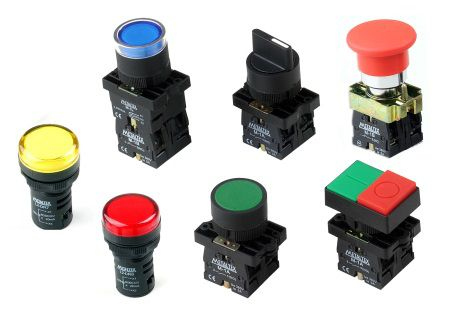
\includegraphics[width=0.6\textwidth]{figuras/botoeiras}
  \caption{Diversos tipos de botoeiras.}\label{fig:botoeiras}
\end{figure}

Chaves de fim de curso são chaves eletromecânicas feitas para serem acionadas por algum produto ou equipamento. São usadas para detectar, por exemplo, a passagem do material sendo processado por um determinado ponto, a posição final de movimentação de algum equipamento, entre outros. Normalmente é implementado como um botão com uma alavanca ou algum outro mecanismo na parte a ser acionada.

\begin{figure}
  \centering
  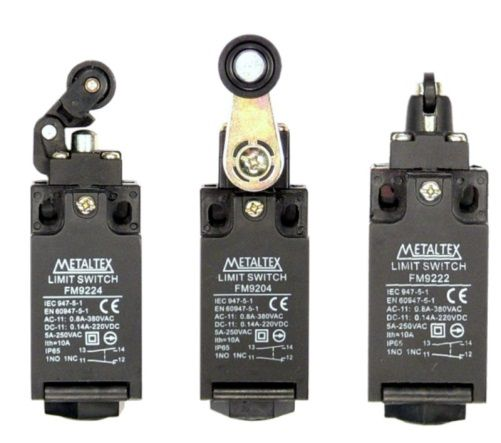
\includegraphics[width=0.6\textwidth]{figuras/fim-de-curso}
  \caption{Exemplos de chaves de fim de curso.}\label{fig:fim-de-curso}
\end{figure}

As chaves eletromecânicas são relativamente baratas, de uma tecnologia já bem amadurecida e são imunes a interferências eletromagnéticas, porém o movimento a que são submetidas gera desgaste, o que faz com que sua vida útil seja reduzida. Além disso, necessitam do contato com o alvo para ser acionadas, o que pode ser inviável em alguns casos, e tem um tempo de resposta da ordem de milisegundos, que pode ser lento demais para algumas aplicações.

\subsection{Sensores de proximidade}

 Existem diversos princípios físicos que podem e são usados para detectar a proximidade de algum material. Estes são chamados de sensores de proximidade e normalmente são aplicados quando se tem algum impedimento ao uso de chaves eletromecânicas.

Para vários casos, é comum o uso de um encapsulamento em formato de rosca, como visto na figura . Isto faz com que vários sensores de proximidade se pareçam, mesmo que usem princípios físicos diferentes.

\begin{figure}
  \centering
  {\Huge FALTA ESTA FIGURA!}%\includegraphics[width=0.6\textwidth]{figuras/proximidade}
  \caption{Encapsulamentos comuns para sensores de proximidade.}\label{fig:proximidade}
\end{figure}

\subsubsection{Indutivo}
\label{subs:Indutivo}
O sensor indutivo conta com uma bobina na sua extremidade sensora, que gera um campo magnético variável na sua frente. A frequência deste campo magnético depende da própria indutância desta bobina, que por sua vez depende do que estiver na frente do sensor.

Um alvo que esteja na frente deste sensor pode alterar esta indutância por 2 efeitos: se for um condutor, gerará um campo magnético contrário, aumentando a indutância; se for ferroelétrico, concentrará o campo magnético, também aumentando a indutância. Este segundo efeito é maior que o primeiro, o que faz com que este sensor responda melhor a ferro do que a cobre, mesmo com o cobre sendo melhor condutor que o ferro.

A distância que um sensor indutivo consegue detectar um alvo de ferro na sua frente é chamada de \textbf{distância sensora nominal}. Para outros materiais esta distância diminui e para materiais não condutoros e sem propriedades magnéticas ela cai a zero. A figura \ref{fig:distancia_sensora} mostra a variação da distância sensora de sensores indutivos e capacitivos para diferentes materiais.

\begin{figure}
  \centering
  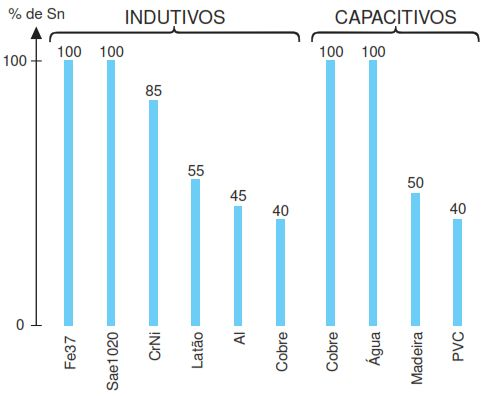
\includegraphics[width=0.6\textwidth]{figuras/distancia_sensora}
  \caption{Variação da distância sensora de sensores indutivos e capacitivos para diferentes tipos de material.}\label{fig:distancia_sensora}
\end{figure}

Além da limitação da distância que pode ser usado e da limitação do material do alvo, sensores indutivos estão sujeitos a interferências eletromagnéticas, que podem gerar falsas detecções.

\subsubsection{Capacitivo}
\label{subs:Capacitivo}

Sensores capacitivos usam um circuito oscilador (basicamente o mesmo de sensores indutivos) para detectar a variação da capacitância entre duas placas metálicas na sua ponta. Esta capacitância varia se o alvo tiver uma constante dielétrica diferente que a do ar. Funciona muito bem para água e cobre (que tem uma constante dielétrica 80 vezes maior que o ar). Praticamente não responde para ferro aço e alumínio.

Pela fraca sensibilidade a papel e plástico, pode detectar a presença de alguns objetos dentro da embalagem. Pela alta sensibilidade à água, é muito usado para detecção de nível. Também é sensível à interferência eletromagnética, embora menos que o indutivo.

\subsubsection{Ultrassônico}
\label{subs:Ultrassonico}

Sensores ultrassônicos detectam a presença de um objeto pelo eco de um sinal ultrassônico (da ordem de \SI{40}{kHz}). Também é muito usado para sensores contínuos de distância, já que o tempo que o eco demora pode ser usado para determinar a distância até o alvo.

Sensores ultrassônicos podem ser usados para detectar alvos em distâncias de até alguns metros, muito embora aí deva se ter o cuidado de que não há outros elementos que possam gerar eco. É sensível não apenas à qualidade do material mas também à geometria do mesmo.

Outro problema em sensores ultrassônicos é que eles tem uma distância mínima de trabalho. Se o alvo estiver muito próximo o sensor não consegue diferenciar o eco do sinal que ele ainda está gerando.

\subsubsection{Óptico}
\label{subs:optico}

Sensores ópticos funcionam com um emissor e um receptor de luz. Tipicamente se usa luz infravermelha, pois a eletrônica baseada em silício é mais sensível a este comprimento de onda, o que barateia o ccusto. Normalmente o sinal luminoso é modulado num trem de pulsos, para diminuir a interferência do sol, cuja luz não é modulada.

\begin{figure}
  \centering
  \includegraphics[width=0.4\textwidth]{figuras/sensorOptico}
  \caption{Princípio de funcionamento do sensor óptico por refexão.}\label{fig:sensorOptico}
\end{figure}

Os tipos mais comuns deste tipo de sensor são:
\begin{description}
  \item[Reflexão difusa] com o emissor do lado do receptor e detecta-se o alvo pelo seu reflexo.
  \item[Retro reflexivo] que é o mesmo caso mas com um anteparo reflexivo atrás. Neste caso o alvo impede a passagem da luz.
  \item[Barreira] que usa o emissor e receptor separados e detecta-se a oclusão do feixe óptico. O uso de um lase como emissor permite alcançar uma grande distância.

  Um uso interessante do sensor óptico de barreira é a chamada barreira laser, onde um conjunto de lasers passando por espelhos cercam um equipamento mais perigoso, de modo que qualquer pessoa ou coisa que acione a barreira enquanto o equipamento está atuando cause uma parada de emergência, diminuindo o risco do equipamento.
\end{description}

Além da luz ser imune a influência eletromagnética, o uso de fibras ópticas pode separar bastante a eletrônica do processo, permitindo o uso deste tipo de sensor em regiões onde não pode ter equipamentos elétricos.

\subsubsection{Magnético}
\label{subs:Magnetico}

Há dois tipos básicos de sensores magnéticos: sensores Hall e \emph{reed switches}. Ambos detectam a presença de um campo magnético, normalmente causado pela aproximação de um imã.

O sensor Hall detecta o campo magnético pela influência do mesmo numa corrente elétrica, pelo chamado efeito Hall. É muito usado para medir a rotação em eixos com um imã acoplado ou em motores elétricos. É um sensor barato, de alta durabilidade e rápido tempo de resposta, porém apenas aplicável a alvos magnetizados.

O \emph{reed switch} é composto de dois contatos de material ferromagnético normalmente separados, tal como mostra a figura \ref{fig:reed}. Um campo magnético perpendicular a estes contatos causam a magnetização dos mesmos, o que faz com que eles se atraiam e fechem contato.

\begin{figure}
  \centering
  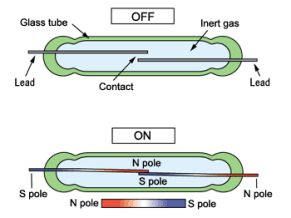
\includegraphics[width=0.5\textwidth]{figuras/reed}
  \caption{\emph{Reed Switch}.}\label{fig:reed}
\end{figure}

O \emph{reed switch} é bem mais barato que o Hall, mas tem pouca durabilidade e elevado tempo de resposta.

\subsection{Chaves de processo}

Chaves de processo são chaves elétricas que atuam quando uma grandeza do processo de fabricação (uma variável de processo) passa determinado nível. Por exemplo: temperatura do tanque 1 acima de \SI{100}{\celsius}, nível do silo abaixo de \SI{2}{\meter}, e assim por diante.

São exemplos de chaves de processo:
\begin{description}
  \item[bóias] que acionam um contato elétrico,
  \item[sensor capacitivo] acionado pelo nível de água de um reservatório,
  \item[chaves de fluxo] onde uma lingueta aciona uma chave eletromecânica se o fluxo passar de um  determinado limite,
  \item[termostatos] que acionam quando a temperatura passa de determinado nível, entre outros.
\end{description}

É cada vez mais comum trocar as chaves de processo por sensores contínuos e implementar o limite de chaveamento no nível de controle da pirâmide. Isto permite uma maior flexibilidade, pois variar o limite no software é mais simples.

\section{Sensores Contínuos}

Sensores contínuos usam algum princípio físico para a medição de alguma grandeza física. As grandezas mais comumente medidas são temperatura, comprimento (nível, espessura, posição), vazão e pressão.

\subsection{Pressão e força}
\label{sub:Pressão e força}
Como pressão é força por área, se se consegue medir um, pode-se usar o mesmo princípio físico para medir outro.

Os principais princípios físicos para a medição de pressão ou força são:
\begin{description}
  \item[Coluna de líquido] usa um tubo fino com um líquido. Ao se colocar o tubo de ponta cabeça, o líquido escorre deixando um vácuo. O comprimento do vácuo é proporcional à pressão externa.

  Normalmente se usa como um indicador. Não é adequado para interfacear com circuitos elétricos.

  \item[Elástico] Utiliza a deformação de um elemento elástico para determinar a pressão. O elemento elástico em si pode ter vários formatos: formato de C, helicoidal, espiral, diafragma.

  Pode ser usado tanto como mero indicador, acoplando o elemento elástico a um ponteiro (Bordon tipo C, por exemplo), ou como um transdutor com uso de uma fita extensiométrica.

  A fita extensiométrica é um resistor que varia a resistência com a tração ou compressão (efeito piezoresistivo). Ao ser colado ao elemento elástico, permite transformar a deformação deste elemento num sinal elétrico.

  \item[Piezoelétrico.] Baseiam-se no efeito apresentado por alguns cristais (normalmente se usa o quartzo) que geram um sinal elétrico ao serem submetidos a uma força e geram uma força quando lhe são aplicados sinais elétricos. Isto permite a construção de circuitos osciladores que variam a sua frequência de ressonância natural em função da força aplicada.
\end{description}

\subsection{Temperatura}
Entre as diversas maneiras de medir temperatura, destacam-se:
\begin{description}
  \item[Tubo capilar], também conhecido como termômetro líquido. Usa um líquido que ao sofrer expansão térmica ocupa um tubo capilar, que permite visualizar a temperatura. Bom para visualização mas não adequado para automação, por não sr fácil gerar um sinal elétrico a partir dele.

  \item[$\Delta V_{BE}$] -- pode-se usar dois transistores bipolares para gerar uma diferença de tensão ($\Delta V_{BE}$) que é proporcional à temperatura absoluta (em Kelvin). É limitado à faixa de temperatura em que a eletrônica funciona: de aproximadamente \SI{-55}{\celsius} a \SI{120}{\celsius}.

  O grande uso da eletrônica fez com que o custo deste tipo de dispositivo caísse bastante, principalmente quando integrado em algum outro circuito. É muito usado em termômetros digitais e no controle de temperatura de processadores de computador.

  \item[Termopar] Pode-se determinar a energia necessária para retirar elétrons de um determinado camada, o que se chama de \emph{função trabalho} do material. Quando dois materiais diferentes se juntam, a diferença da função trabalho deles gera um potencial elétrico. Normalmente este potencial elétrico não é percebido pois ao se fazer um circuito fechado de diferentes materiais com todas as junções na mesma temperatura, estas diferenças acabam se anulando. Porém, se pegarmos dois fios condutores com diferentes funções trabalhos,unirmos uma ponta e colocarmos esta junção numa temperatura diferente, como num forno, por exemplo, aparece uma tensão que é função dos materiais usados e da diferença de temperatura. Este é o chamado efeito Seebeck:
  \[
E = (S_\mathrm{B} - S_\mathrm{A}) \cdot (T_2 - T_1),
  \]
  onde E é a tensão gerada, $S_\mathrm{A}$ e $S_\mathrm{B}$ são os coeficientes de Seebeck dos materiais A e B e $T_2$ e $T_1$ são as diferentes temperaturas.

Logo o termopar mede a diferença de temperatura entre dois lugares e não a temperatura absoluta., precisando de um medidor auxiliar para medir a temperatura ambiente.

Existem diversos tipos de termopar, formados por diferentes junções de metais. Há vários tipos padrões identificados por uma letra: J - ferro e constantan; K - Níquel-Cromo e Níquel-Alumínio; S - Platina e Ródio e Platina. Escolhe-se o tipo pela faixa de operação, precisão e custo.

  \item[Termorresistor] utiliza a variação da resistência de um condutor com a temperatura. Usa um polinômio que relaciona a resistência com a temperatura, como:
  \[
R = R_0[1+a\cdot T+b\cdot T^2],
  \]
onde T é a temperatura em Celsius e $R_0$ é a resistência quando a temperatura é de \SI{0}{\celsius}.

São usados metais inertes, tais como o níquel ou a platina. O nome do sensor é o símbolo do elemento químico usado seguido da resistência à \SI{0}{\celsius}: Pt100, Ni500, etc.
  \item[Pirômetro] ou termômetro de infravermelho usa a chamada raiação do corpo negro para determinar a temperatura. Todo objeto emite fótons de comprimento de onda relacionado à temperatura do objeto. O pirômetro mede então o comprimento de onda destes fótons, permitindo a medição da temperatura à distância.

  Apesar da praticidade ainda são bastante caros. Hoje se usa também as câmeras térmicas, baseadas no mesmo princípio.
\end{description}

\section{Transmissão de dados, aterramento e blindagem em instrumentação.}

\section{Diagrama P\&ID}

Um PI\&D (\emph{Piping and Instrumentation Diagram}) é um diagrama que coloca de forma bem compacta várias informações sobre os instrumentos ligados a um processo. Um exemplo pode ser visto na figura \ref{fig:exemploPID}. Neste diagrama, os instrumentos são representados por símbolos padrões, definidos pela norma ISA 51.

\begin{figure}[h]
  \centering
  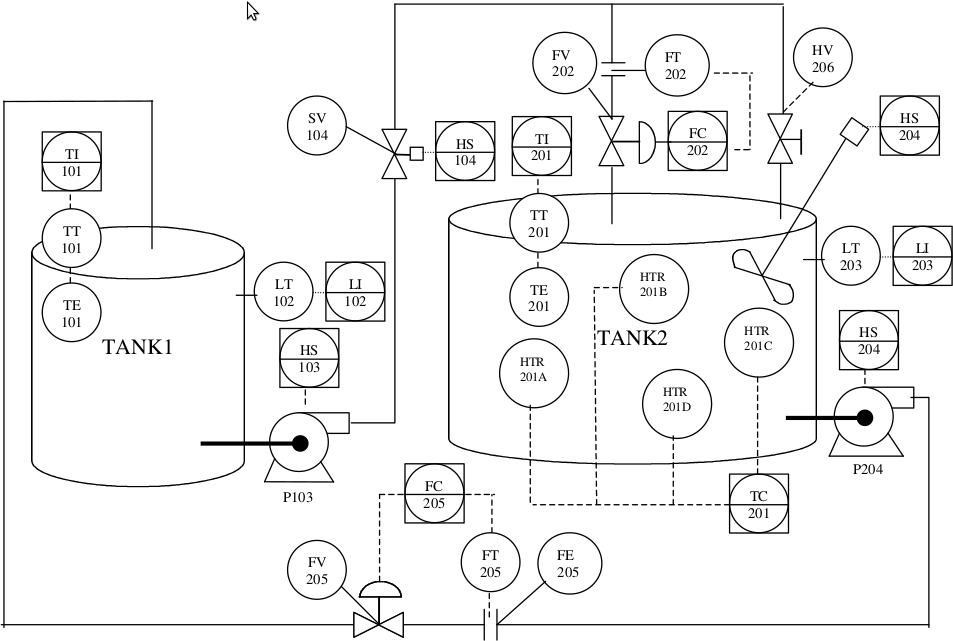
\includegraphics[width = 0.8\textwidth]{figuras/exemploPID}
  \caption{Exemplo de um diagrama P\&I.\label{fig:exemploPID}.}
\end{figure}

Cada instrumento é definido por um conjunto de letras e um número. A primeira letra indica que grandeza é relacionada àquele instrumento; a segunda letra em diante especifica a função daquele instrumento, com eventuais modificadores.
Exemplos:
\begin{description}
  \item[TRC --] \emph{Temperature Register and Controller}, controlador e registrador de temperatura.
  \item[PDIC --] \emph{Pressure (differential) Indicator and Controller}, controlador e indicador de pressão diferencial.
  \item[FAH --] \emph{High Flow Alarm}, alarme de vazão alta.
\end{description}

As funções mais comuns de um instrumento são:
\begin{description}
  \item[A -- Alarme.]
  \item[C -- Controlador.] Responsável por gerar o sinal de controle do atuador que afeta aquela variável.
  \item[I -- Indicador.] O instrumento permite ler o valor da variável nele.
  \item[T -- Transmissor.] O instrumento é um transdutor que gera um sinal padrão para outro instrumento.
\end{description}

O número é referente a malha de instrumentação. Normalmente é relacionado com a variável de processo que é controlada por aquele conjunto de instrumentos. Na própria figura \ref{fig:exemploPID}, na parte superior, o conjunto de instrumentos FT202, FC202 e FV202 fazem a malha de controle que mede (FT202), controla (FC202) e atua (FV202) na vazão de água do tanque 1 para o 2.

Vários instrumentos tem símbolos próprios, tais como bombas e válvulas. Outros instrumentos são representados por um símbolo (figura \ref{fig:simbolosISA}), contendo o código do mesmo, que indicam o que é o instrumento e onde ele está localizado.
\begin{figure}[h]
  \centering
  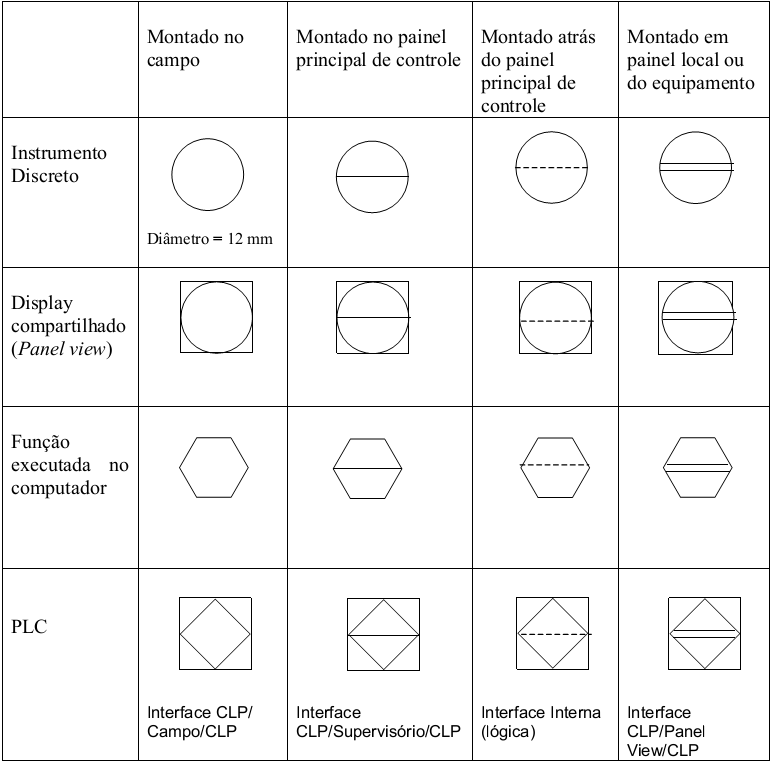
\includegraphics[width = 0.6\textwidth]{figuras/simbolosISA}
  \caption{Explicação dos símbolos dos instrumentos.\label{fig:simbolosISA}.}
\end{figure}

\subsection{Transmissão de dados}
\label{sub:TransmissaoDeDados}

A forma como os sinais são transmitidos entre os instrumentos é indicada porum padrão. A linha que liga os instrumentos são decoradas de acordo com a forma com que a informação passa de um instrumento para o outro, de acordo com a figura \ref{fig:linhasISA}.
\begin{figure}[h]
  \centering
  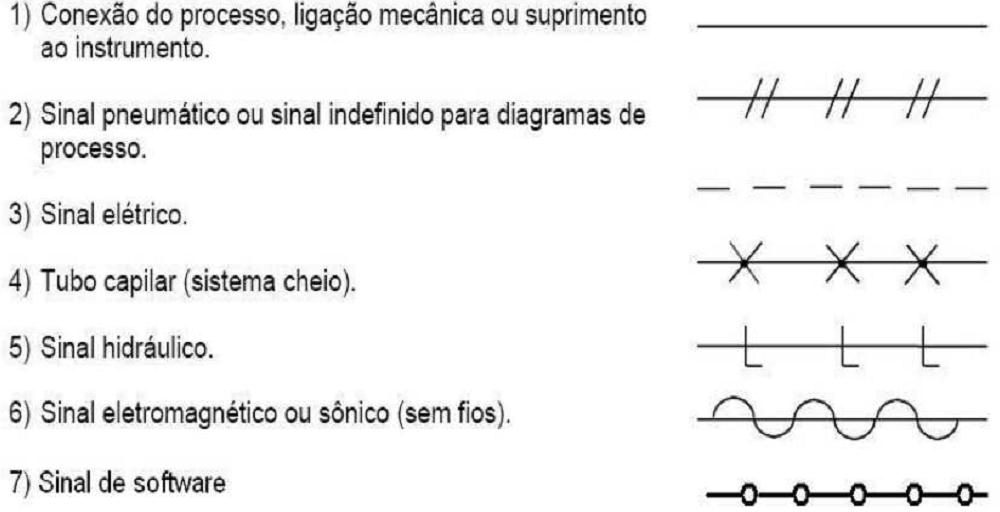
\includegraphics[width = 0.6\textwidth]{figuras/linhasISA}
  \caption{Explicação das linhas do diagrama P\&I.\label{fig:linhasISA}.}
\end{figure}

Sinais comuns são:
\begin{description}
  \item[Pneumáticos.] Usam gás comprimido na faixa de 20 a \SI{100}{\kilo\pascal}. É usado em áreas que se tenha risco de explosão. Tem limitação com a distância e é difícil de detectar vazamentos.

%  A razão de usar uma pressão mínima maior que a ambiente (aproximadamente \) é para facilitar a detecção de erros: Se o transmissor não funcionar a pressão vai cair para abaixo de \SI{20}{\kilo\pascal}
  \item[Hidráulico.] Usam óleo sobre pressão. São mais caros que sistemas pneumáticos porém são mais rápidos e podem ser usados para acionar equipamentos de grande porte.
  \item[Elétrico.] Usam um sinal de 4 a \SI{20}{mA} ou de 1 a \SI{5}{\volt}. Em geral o de corrente, pois são menos sujeitos a interferências.

  Os receptores deste tipo de sinal tem internamente um resistor de \SI{250}{\ohm} em paralelo a sua entrada, o que permite que aceitem ambos tipos.

  A razão de usar um valor mínimo maior que zero é para facilitar a detecção de falhas no transmissor, que normalmente fazem o sinal ir para 0.

  \item[Sinais digitais.] São sinais elétricos modulados de acordo com um protocolo de comunicação digital. São usados nos chamados sensores inteligentes e estão ficando cada vez mais comuns.

  Dependendo do protocolo usado, podem ter um custo total menor que o elétrico analógico por redução de cabeamento. Além disto, a comunicação digital permite passar outras informações, tais como configurações, dados de calibração e diagnósticos.

  Existem muito protocolos diferentes no mercado, com pouca compatibilidade entre eles.

  \item[Rádio.] Normalmente usam sinais digitais modulados em rádio frequência. São muito usados para longas distâncias e para equipamentos móveis. Interferência e problemas de segurança diminuem seu uso mais geral.
\end{description}

\chapter{Controladores Lógico-Programáveis (CLP)}
%!TEX root = principal.tex
\section{Dispositivos Eletromecânicos}

Há vários dispositivos eletromecânicos de interesse para a automação industrial, dos quais destacamos motores elétricos, solenóides, chaves e relês.

Destes, motores e solenóides são atuadores e chaves são sensores. Relês podem ser usados tanto como atuadores como como sensores, embora sejam mais usados em atuadores.

Chaves já foram vistas junto com instrumentação, enquanto motores são assuntos de outras disciplinas e fogem do escopo desta disciplian.

Solenóides são basicamente eletroimãs com um eixo ferromagnético preso a uma mola. O eixo pode ter duas posições: uma mantida pela mola, que é a posição que ele assume quando o eletroimã não é acionado, e outra forçando a mola, quando o eletroimã é acionado. Ou seja: são dispositivos de acionamento binários.

Solenóides tipicamente fornecem uma movimentação de no máximo poucos centímetros a cargas de miligramas a dezenas de kilogramas. São muito usados para acionamento de válvulas - válvulas solenóides.

Relês eletromecânicos são, por construção, solenóides no qual o eixo faz abrir ou fechar contatos elétricos. Eles são chaves elétricas acionadas eletricamente. Hoje em dia existem relês baseados em eletrônica, chamados de relês de estado sólido, que tem a mesma função mas por princípios de funcionamento bem diferentes. Eletricamente pode-se visualizar um relê apenas como um indutor (a bobina do eletroimã) e um contato, e muitas vezes é desta forma que ele é representado em um diagrama esquemático (vide exemplo na Figura \ref{fig:diagRele}).

O estado de repouso dos cantatos define o tipo básico do relê: normalmente aberto ou normalmente fechado. É comum relês que tenham 2 ou mais contatos acionadas por uma mesma bobina, inclusive podendo ser uma normalmente aberta e outra normalmente fechada, tal como o relê da figura \ref{fig:fotoRele}.

\begin{figure}[!h]
  \centering
  \subfloat[Foto de um relê\label{fig:fotoRele}]{  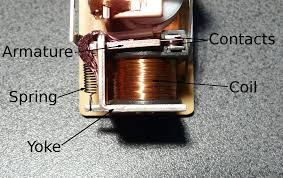
\includegraphics[scale=0.6]{figuras/relay}}
  \subfloat[Diagrama esquemático\label{fig:diagRele}]{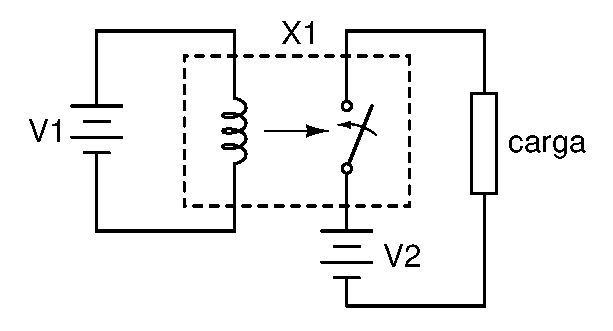
\includegraphics[scale=0.6]{figuras/rele}} %%TODO: refazer
  \caption{Foto de um relê e representação esquemática.}
\end{figure}

Uma grande utilidade dos relês vem do fato que a bobina de acionamento é eletricamente isolada dos cantatos, o que permite usar relês para:
\begin{itemize}
  \item Controle de alta tensão e/ou potência através de baixa tensão e/ou potência -- um sinal de mW pode comandar kW de potência através de um relê.
  \item Isolação e proteção do circuito de controle.
  \item Acionamento trifásico -- um contator é um relê com três conjuntos isolados de contatos acionados pela mesma bobina.
  \item Implementação de lógica de controle -- são os chamados circuitos chaveados.
\end{itemize}
\section{De relês a CLPs}

Um exemplo de aplicação de relê é mostrado na figura \ref{fig:releCircuito1}, onde 2 relês c1 e c2 são usados para o acionamento de um motor trifásico comandado pelas botoeiras b0, b1 e b2.

\begin{figure}[hbt]
  \begin{center}
    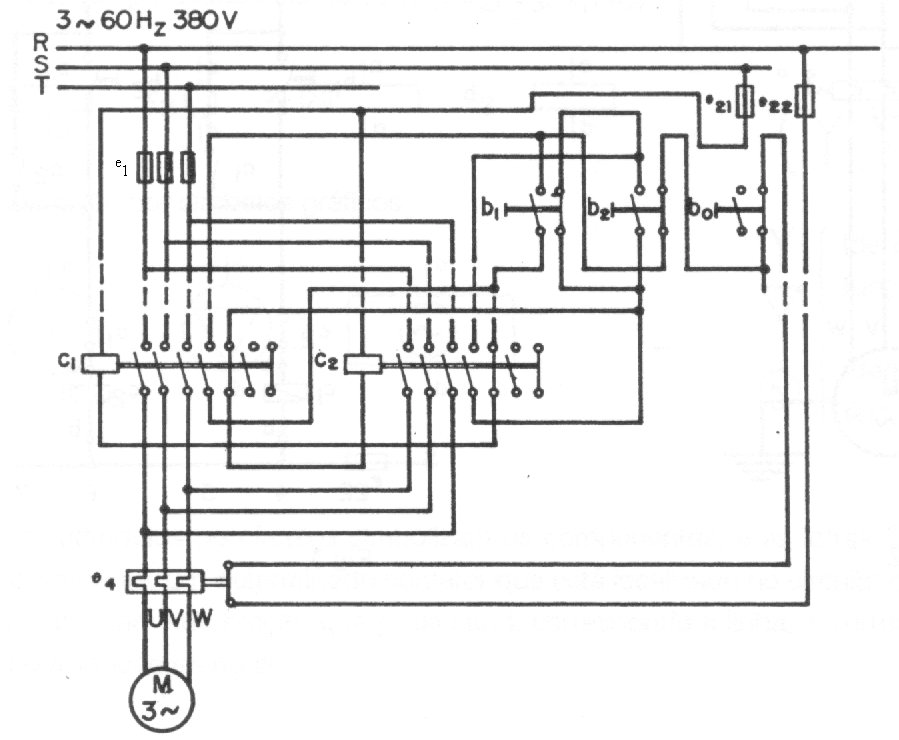
\includegraphics[width=0.8\textwidth]{figuras/releCircuito1} %%TODO: refazer
  \end{center}
  \caption{Circuito de acionamento de um motor trifásico por relê.}
  \label{fig:releCircuito1}
\end{figure}

Em geral é mais fácil analisar um circuito do ponto de vista lógico separando a parte de acionamento da parte de controle, então é comum que o símbolo de um relê seja separado em duas partes: a bobina (o eletroímã) e o contato (a chave), interligados pelo mesmo nome. Isto é exemplificado na figura \ref{fig:releCircuito2}, que redesenha o mesmo circuito da figura \ref{fig:releCircuito1} separando a parte de controle da de acionamento, tornando o circuito bem menos convoluto. A ligação entre os diversos contatos e bobinas dos relês permite a realização de diversas funções interessantes para o controle de circuito. Tais circuitos ficaram conhecidos por \emph{circuitos chaveados}.

\begin{figure}[hbt]
  \begin{center}
    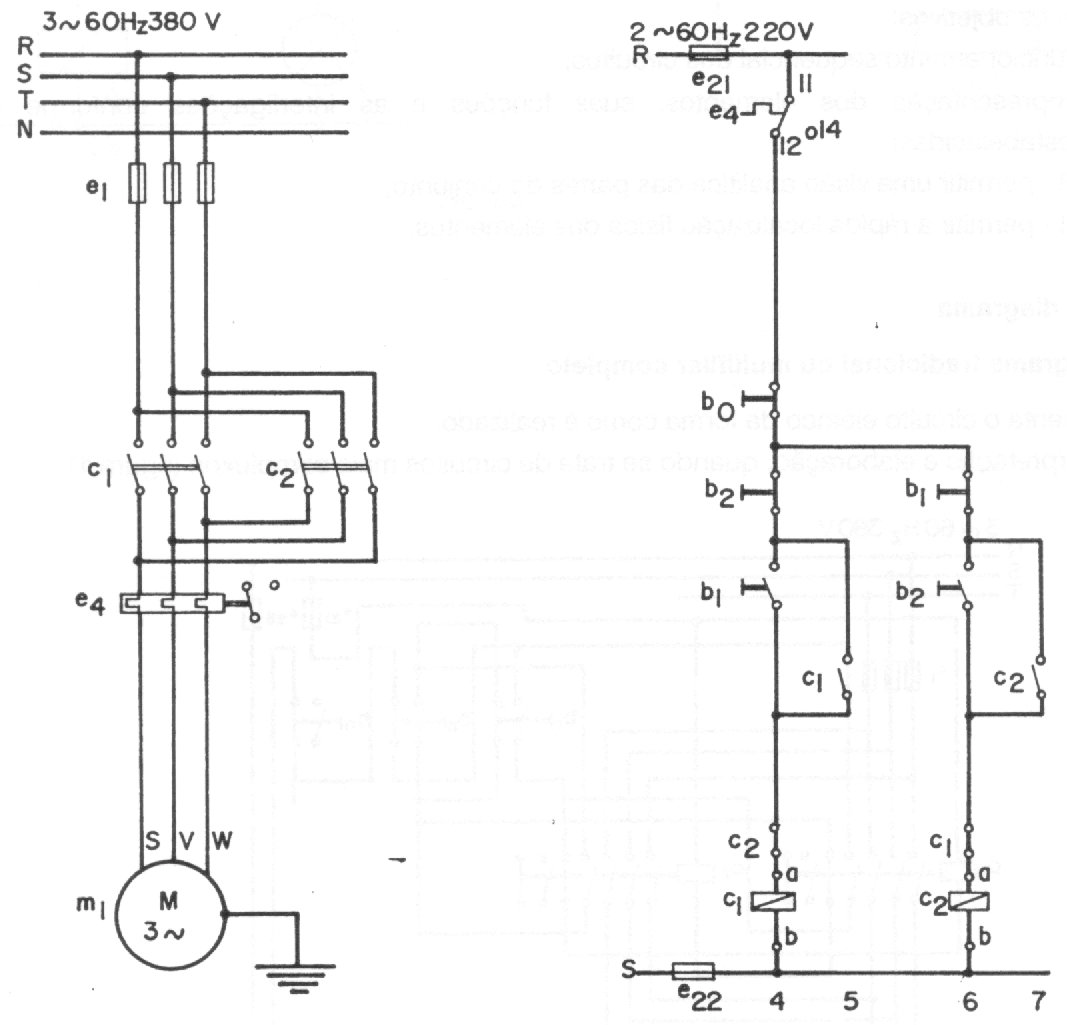
\includegraphics[width=0.8\textwidth]{figuras/releCircuito2} %%TODO: refazer
  \end{center}
  \caption{Mesmo circuito da figura \ref{fig:releCircuito1}, separando a parte de controle da de acionamento.}
  \label{fig:releCircuito2}
\end{figure}

\subsection{Diagrama Ladder}
\label{sec:diagrama-ladder}

Os diagramas ladder são muito utilizados para representar circuitos com relês enfantizando a lógica da ligação. Neste tipo de diagrama as bobinas tem o símbolo 
\includegraphics[height=0.9em]{figuras/bobina_ladder}, os contatos normalmente abertos são simbolizados por 
\includegraphics[height=0.9em]{figuras/na_ladder} e os normalmente fechados por 
\includegraphics[height=0.9em]{figuras/nf_ladder}.

A Figura \ref{fig:ladder1} mostra o mesmo circuito de controle da Figura \ref{fig:releCircuito2}, só que agora descrito em ladder. Com os circuitos conectados desta maneira, o diagrama fica parecendo uma escada; daí o nome\footnote{em inglês \emph{ladder} significa escada.}.


\begin{figure}[!h]
  \centering
  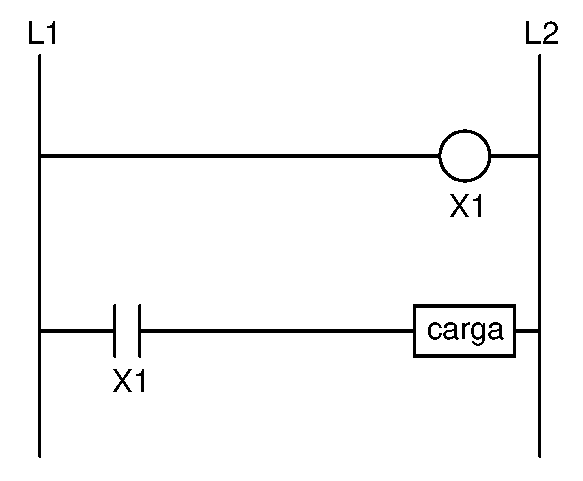
\includegraphics[scale=0.6]{figuras/ladder1} %%TODO: Refazer para ser o mesmo da figura ref:releCircuito2
  \caption{Exemplo de circuito de controle em ladder.}
  \label{fig:ladder1}
\end{figure}

Logo de cara nota-se que não existem neste diagrama as tensões V1 e V2. Isto se dá pois neste diagrama considera-se que as tensões estão entre as duas barras L1 e L2 e abstrai-se a fonte de tensão. Isto lembra, de certo modo, a ligação real, com os elementos conectados entre os cabos de fase e o neutro.


Como exemplo, a figura \ref{fig:ladders} mostra diagramas ladder que acendem uma lâmpada apenas quando 2 relês são acionados, se qualquer um dos relês for acionado ou quando nenhum dos relês é acionado.

\begin{figure}[!h]
  \centering
  \subfloat[Aciona apenas se ambos relês estiverem acionados.]{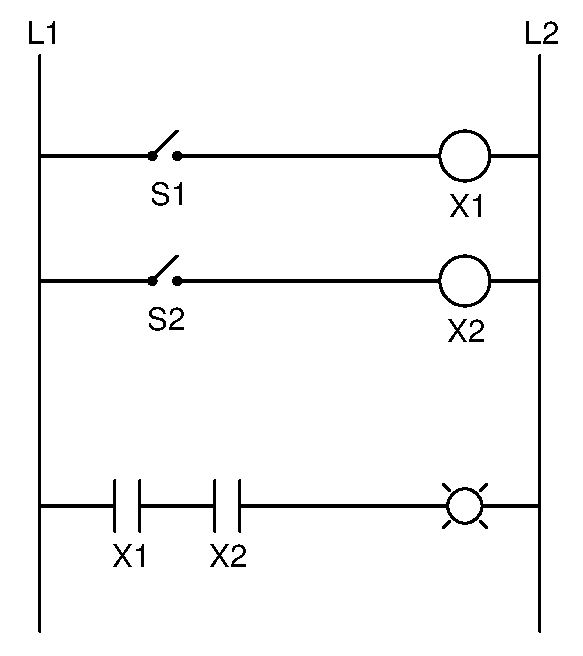
\includegraphics[scale=0.6]{figuras/ladder_e}}
  \subfloat[Aciona se um ou outro relê estiver acionado.]{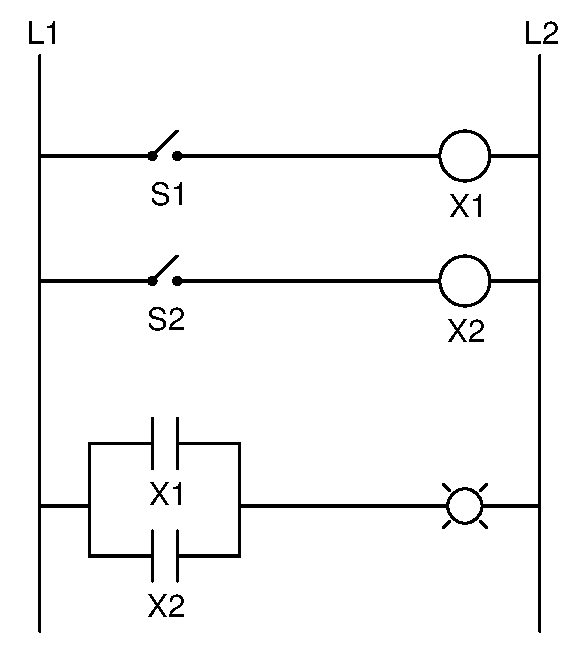
\includegraphics[scale=0.6]{figuras/ladder_ou}}
  \subfloat[Aciona se o relê não estiver acionado.]{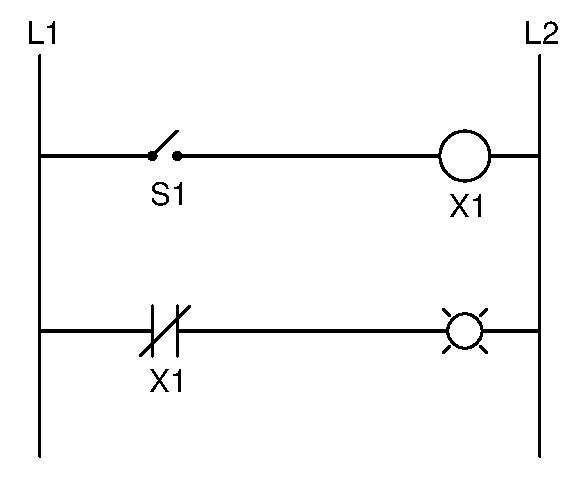
\includegraphics[scale=0.6]{figuras/ladder_nao}}
  \caption{Exemplos de circuitos lógicos chaveados em ladder.}
  \label{fig:ladders}
\end{figure}


O engenheiro Claude Shannon descobriu em 1934 a relação entre os circuitos chaveados e a álgebra de Boole, que é um mapeamento da lógica em uma álgebra. Uma ligação em série realiza um $\mathrm{AND}$ lógico (uma multiplicação booleana), uma ligação paralela realiza um $\mathrm{OR}$ lógico (uma soma na álgebra de Boole) e o uso de um contato normalmente fechado realiza a inversão lógica, ou o $\mathrm{NOT}$ (representado por uma barra sobre a variável). A álgebra de Boole mostra que a combinação destas três operações, e portanto a combinação destes três circuitos, permite realizar qualquer condição lógica para o acionamento do que quer que seja, muito embora a aplicação direta dos postulados e teoremas desta álgebra não seja muito intuitiva.

Porém, apesar da facilidade deste diagrama, a montagem física ainda era bastante complexa, uma vez que o acionamento e os contatos de um relê são obrigatoriamente parte de um único dispositivo físico, e que para lógicas mais complexas essa fiação se tornava bastante complicada. Isto é ainda mais preocupante quando se precisa alterar a lógica de funcionamento, pois se tem que mexer no circuito como um todo.

Além disso, por ser um dispositivo eletromecânico, relês não tem um elevado tempo de vida: pode chavear talvez menos que 10 000 vezes, dependendo da tensão e corrente que suporta.

Em 1947, foi inventado o transistor, que age, como o relê, como uma chave elétrica controlada eletricamente. Principalmente pelo fato de não ter partes móveis, um transistor tem um tempo de vida muito mais longo que um relê, além de ter um chavemaneto mais rápido. Isto permitiu a construção de computadores eletrônicos muito mais rápidos, confiáveis e robustos que os a relê. O problema para o uso na automação é que os transistores não aguentam tensões e correntes tão elevadas quanto os relês.

Em 1968, a GM lançou uma especificação de um elemento de controle que pudesse substituir relês. Esta especificação pedia por:
\begin{itemize}
  \item Facilidade de programação;
  \item Facilidade na manutenção (encaixe de módulos);
  \item Confiabilidade maior;
  \item Mais compacto;
  \item Possibilitar o envio de dados à central de processamento;
  \item Economicamente competitivo;
  \item Entradas em tensão alternada 115 V;
  \item Saídas  em 115 V C.A. com mais que 2 A (operação das válvulas solenóides, comando para partida de motores e outros);
  \item Possibilitar a ampliação com um mínimo de alteração;
  \item Dotado de memória;
\end{itemize}

A partir desta especificação, foi desenvolvido pela Bedford Associates o primeiro PLC, posteriormente vendido pela marca MODICON -- \emph{MOdular DIgital CONtroller}. Ele usa um microcontrolador para realizar a lógica e conta com dispositivos modulares de interface de entrada e saída. A figura \ref{fig:plc_sistema} mostra a arquitetura típica de um CLP.

\begin{figure}[hbt]
  \centering
  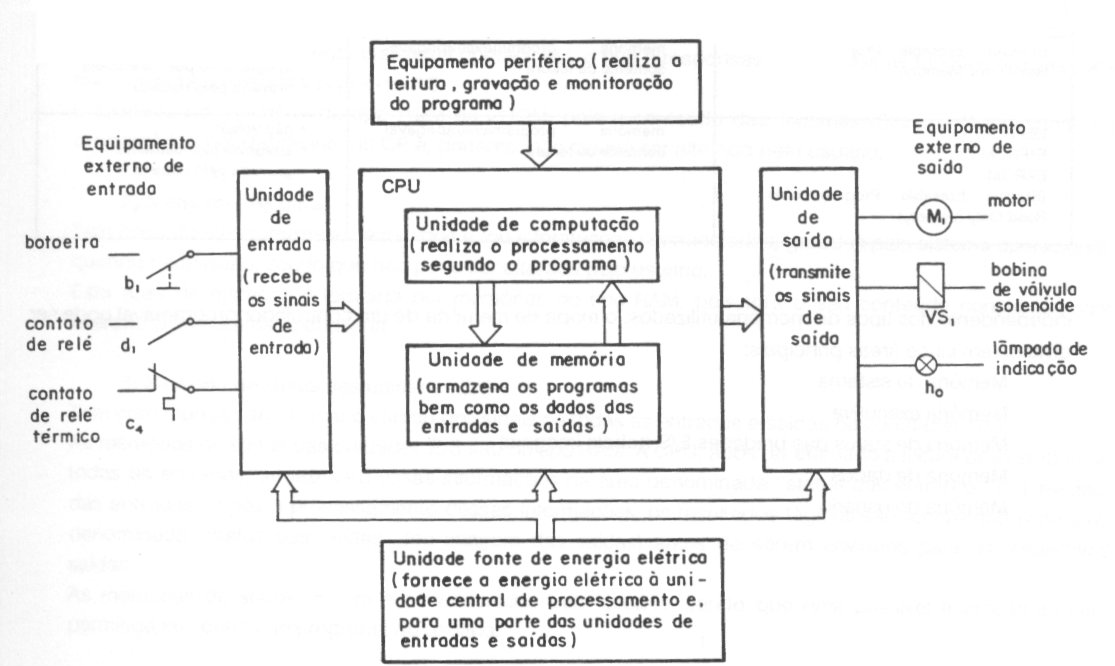
\includegraphics[width=\textwidth]{figuras/plc_sistema}
  \caption{Arquitetura interna de um CLP.}
  \label{fig:plc_sistema}
\end{figure}

As entradas e saídas dos CLPs são isoladas eletricamente, uma vez que o microcontrolador não suporta altas tensões ou correntes. Tipicamente ainda são usados relês para a implementação das saídas digitais, mas cada vez mais se tem soluções totalmente eletrônicas. A Figura \ref{fig:ESclp} mostra circuitos típicos de entrada e saída.
\begin{figure}[h]
  \centering
  \begin{tabular}{cc}
  \subfloat[Entrada de tensão contínua.]{  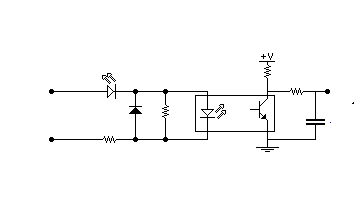
\includegraphics[width=0.45\textwidth]{figuras/entrada_clp_cc}} &
  \subfloat[Entrada de tensão alternada.]{  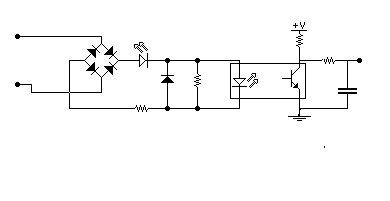
\includegraphics[width=0.45\textwidth]{figuras/entrada_clp_ca}} \\
  \subfloat[Saída a relê.]{  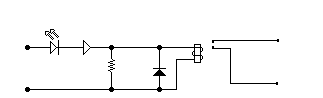
\includegraphics[width=0.45\textwidth]{figuras/saida_clp_rele}} &
  \subfloat[Saída de tensão contínua.]{  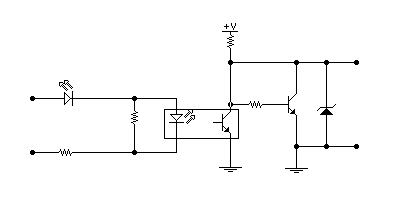
\includegraphics[width=0.45\textwidth]{figuras/saida_clp_cc}}\\
  \end{tabular}
  \caption{Entradas e saídas típicas de CLPs.}
  \label{fig:ESclp}
\end{figure}

\section{IEC61131}
A IEC61131, antes conhecida por IEC1131 é uma norma técnica do \emph{International Eletrotechnical Commission}, que define um padrão para CLPs. Esta norma define vários requisitos de hardware e software para os CLPs, desde aspectos de segurança até guias de uso.

No CLP há um programa principal que continuamente executa a seguinte sequência:
\begin{enumerate}
  \item Faz um auto-teste.
  \item Se comunica com outros dispositivos, se houverem. Estes outros dispositivos podem ser: computador, outro CLP, IHM, etc.
  \item Lê as entradas, armazenando uma cópia das entradas em posições de memória.
  \item Executa o(s) código(s) do usuário.
  \item Atualiza as saídas, em função das entradas e do código do usuário.
\end{enumerate}
O código do usuário é composto por um conjunto de blocos em 5 possíveis linguagens, descritas na norma:
\begin{description}
  \item[IL -- Instruction List] Uma linguagem de baixo nível de abstração, parecida com assembly.
  \item[ST -- Structured Text] Uma linguagem textual de alto nível, tal como C ou Pascal.
  \item[LD -- Ladder] O mesmo diagrama de circuitos a relê.
  \item[FBD -- Function Block Diagram] Parecido com um diagrama de portas lógicas: blocos com entradas e saídas.
  \item[SFC -- Sequential Function Chart] Baseado em Grafcet, uma extensão de máquina de estados.
\end{description}

A idéia por trás desta estrutura é que o tempo que o CLP passe executando esta sequência (conhecido por \emph{scan time}) seja tão pequeno a ponto de poder ser desprezível. Neste contexto o código do usuário deve ser visto como tendo uma execução imediata. Obviamente isto não é verdade, já que o processador que executa este código é uma máquina de Turing -- que é inerentemente sequencial. Mas o \emph{scan time} pode ser da ordem de milissegundos ou dezenas de milissegundos, o que é bem rápido para uma grande quantidade de processos. Isto é especialmente importante quando se trabalha com a linguagem ladder, cuja estrutura remete a um circuito elétrico que é inerentemente paralelo.
%Com este tipo de diagrama, fica fácil analisar a lógica por trás dos circuitos, o que fez com que este diagrama ainda seja usado, só que agora como uma linguagem gráfica de programação de CLPs.

% \section{Mapas de Karnaugh}

% O chamado mapa de Karnaugh foi desenvolvido pelo matemático e físico Maurice Karnaugh em 1953, enquanto trabalhava no grupo de pesquisas da empresa Bell. Este método é uma poderosa ferramenta para circuitos lógicos. %, pois permite simplificar equações booleanas apenas agrupando áreas comuns, o que nosso cérebro consegue fazer bem mais rapidamente do que aplicando postulados e teoremas a equações.

% Como as equações da álgebra de Boole tratam, também, de probabilidade, elas podem ser visualizadas através de um diagrama de Venn. Isto é exemplificado na figura \ref{fig:Venn_mintermos}, que apresenta um diagrama de Venn de 3 variáveis com todas as regiões demarcadas.

% \begin{figure}[!h]
% 	\centering
%   \subfloat[Regiões das variáveis]{\begin{tikzpicture}[scale=1,every node/.style={fill=white,rounded corners}]
%    \draw(0,0)rectangle(4,4);%\draw[step=5mm, red] (0,0) grid (4,4);
%    \draw[pattern=horizontal lines](1.5,1.7)circle(1.2cm);\draw(1,1.2)node{$a$};
%    \draw[pattern=vertical lines](2.5,1.7)circle(1.2cm);\draw(3,1.2)node{$b$};
%    \draw[pattern=north east lines](2,2.5)circle(1.2cm);\draw(2,3.2)node{$c$};
%    \end{tikzpicture}}
% \subfloat[Sub-regiões dos ANDs.]{\begin{tikzpicture}[scale=1,every node/.style={fill=white,rounded corners}]
%    \draw(0,0)rectangle(4,4);%\draw[step=5mm, red] (0,0) grid (4,4);
%    \draw[pattern=horizontal lines](1.5,1.7)circle(1.2cm);
% \draw(1,1.2)node{\scriptsize{$a\comp{b}\comp{c}$}};
%    \draw[pattern=vertical lines](2.5,1.7)circle(1.2cm);
% \draw(3,1.2)node{\scriptsize{$\comp{a}b\comp{c}$}};
%    \draw[pattern=north east lines](2,2.5)circle(1.2cm);
% \draw(2,3.2)node{\scriptsize{$\comp{a}\comp{b}c$}};
   
%    \draw(2,1)node{\scriptsize{${a}{b}\comp{c}$}};
%    \draw(1.2,2.5)node{\scriptsize{${a}\comp{b}{c}$}};
%    \draw(2.8,2.5)node{\scriptsize{$\comp{a}{b}{c}$}};
%    \draw(2,2)node{\scriptsize{${a}{b}{c}$}};
%    \draw(2,0.25)node{\scriptsize{$\comp{a}\comp{b}\comp{c}$}};
%    \end{tikzpicture}}
% 	\caption{Diagrama Venn com 3 variáveis.}
% 	\label{fig:Venn_mintermos}
% \end{figure}

% Utilizando os diagramas, é fácil obter a equação simplificada da função. Por exemplo, considere-se a função $f_1=a\comp{b}\comp{c}+a\comp{b}c+\comp{a}\comp{b}c$. Desenhando esta função num diagrama de Venn (figura \ref{fig:Venn_f1}), fica óbvio que podemos simplificá-la para $f_1=(a+c)\comp{b}$.

% \begin{figure}[!h]
% 	\centering
% 	\begin{tikzpicture}[scale=1.4,every node/.style={rounded corners}]
%    \coordinate (a) at ($ (2,2)+(-150:0.6cm)$);
%    \coordinate (b) at ($(2,2)+(-30:0.6cm)$);
%    \coordinate (c) at (2,2.6);
%    \draw(0,0)rectangle(4,4);%\draw[step=1mm, red] (0,0) grid (4,4);
%    \node(a1) at (a)[draw,circle,minimum size=2.4*1.4cm]{};%\draw(1,1.2)node{$a$};
%    \node(b1) at (b)[draw,circle,minimum size=2.4*1.4cm]{};
%    \node(c1) at (c)[draw,circle,minimum size=2.4*1.4cm]{};

%    \fill[pattern=north east lines](intersection 1 of a1 and b1)arc(295:125:1.2cm)arc(176:4:1.2cm)arc(55:244:1.2cm);\draw(2,2)+(150:1cm)node[fill=white]{$f_1$};
% \end{tikzpicture}
% 	\caption{Diagrama Venn definindo a região dada por $f_1=a\comp{b}\comp{c}+a\comp{b}c+\comp{a}\comp{b}c=(a+c)\comp{b}$.}
% 	\label{fig:Venn_f1}
% \end{figure}

% O problema aparece quando acrescentamos mais 1 variável. Como fazer um diagrama definindo todas as 16 possibilidades? Uma solução para isto é desenhar as regiões como retângulos e não como círculos, assim como foi feito na figura \ref{fig:Venn4}, lado esquerdo. Uma melhora é ainda aplicada no diagrama do lado direito desta figura, onde a indicação de que regiões correspondem a que variáveis é feita não pelo padrão da área, mas sim indicada no lado externo.

% \begin{figure}[!hbt]
% 	\centering
% %\subfloat{  
% \begin{tikzpicture}[scale=1.3,every node/.style={rounded corners,fill=white}]
%   \draw(0,0)rectangle(4,4);%\draw[step=1mm, red] (0,0) grid (4,4);
%   \draw[rounded corners,pattern=north east lines](0.05,0.05)rectangle(3.95,2);
%   \draw[rounded corners,pattern=north west lines](2,0.05)rectangle(3.95,3.95); 
%   \draw[rounded corners,pattern=horizontal lines](0.05,1)rectangle(3.95,3);
%   \draw[rounded corners,pattern=vertical lines](1,0.05)rectangle(3,3.95); 
% \kmin{\small{$\comp{a}\comp{b}\comp{c}\comp{d}$}}{\small{$\comp{a}\comp{b}\comp{c}{d}$}}{\small{$\comp{a}\comp{b}{c}\comp{d}$}}{\small{$\comp{a}\comp{b}{c}{d}$}}{\small{$\comp{a}{b}\comp{c}\comp{d}$}}{\small{$\comp{a}{b}\comp{c}{d}$}}{\small{$\comp{a}{b}{c}\comp{d}$}}{\small{$\comp{a}{b}{c}{d}$}} %Coloca os valores dos quadros menos significativos
% \kmax{\small{${a}\comp{b}\comp{c}\comp{d}$}}{\small{${a}\comp{b}\comp{c}{d}$}}{\small{${a}\comp{b}{c}\comp{d}$}}{\small{${a}\comp{b}{c}{d}$}}{\small{${a}{b}\comp{c}\comp{d}$}}{\small{${a}{b}\comp{c}{d}$}}{\small{${a}{b}{c}\comp{d}$}}{\small{${a}{b}{c}{d}$}} %Coloca os valores dos quadros mais significativos
% %\end{tikzpicture}}
% %\subfloat{\begin{tikzpicture}[scale=1.2,every node/.style={rounded corners,fill=white}]
% \begin{scope}[xshift=5cm]
%   \draw(0,0)rectangle(4,4);%\draw[step=1mm, red] (0,0) grid (4,4);
%   \draw[rounded corners,](0.05,0.05)rectangle(3.95,2);
%   \draw(-0.1,0)--(-0.1,1)node[left]{$a$}--(-0.1,2);
%  \draw(4.1,1)--(4.1,2)node[right]{$b$}--(4.1,3);
%  \draw(2,-0.1)--(3,-0.1)node[below]{$c$}--(4,-0.1);
%  \draw(1,4.1)--(2,4.1)node[above]{$d$}--(3,4.1);
%   \draw[rounded corners,](2,0.05)rectangle(3.95,3.95); 
%   \draw[rounded corners,](0.05,1)rectangle(3.95,3);
%   \draw[rounded corners,](1,0.05)rectangle(3,3.95); 
% \kmin{\small{$\comp{a}\comp{b}\comp{c}\comp{d}$}}{\small{$\comp{a}\comp{b}\comp{c}{d}$}}{\small{$\comp{a}\comp{b}{c}\comp{d}$}}{\small{$\comp{a}\comp{b}{c}{d}$}}{\small{$\comp{a}{b}\comp{c}\comp{d}$}}{\small{$\comp{a}{b}\comp{c}{d}$}}{\small{$\comp{a}{b}{c}\comp{d}$}}{\small{$\comp{a}{b}{c}{d}$}} %Coloca os valores dos quadros menos significativos
% \kmax{\small{${a}\comp{b}\comp{c}\comp{d}$}}{\small{${a}\comp{b}\comp{c}{d}$}}{\small{${a}\comp{b}{c}\comp{d}$}}{\small{${a}\comp{b}{c}{d}$}}{\small{${a}{b}\comp{c}\comp{d}$}}{\small{${a}{b}\comp{c}{d}$}}{\small{${a}{b}{c}\comp{d}$}}{\small{${a}{b}{c}{d}$}} %Coloca os valores dos quadros mais significativos
%  \end{scope}
% \end{tikzpicture}
% \caption{Diagrama Venn de 4 variáveis desenhado com regiões quadradas.}
% 	\label{fig:Venn4}
% \end{figure}

% O mapa de Karnaugh já é este diagrama de Venn modificado, onde o resultado da função booleana mapeada é marcado em cada região (casa). Cada casa em um mapa de Karnaugh corresponde a uma linha na tabela verdade, que é um AND de todas as variáveis envolvidas -- vamos chamar isto de mintermo. A figura \ref{fig:karnaugh_mintermos} mostra os mintermos correspondentes a cada uma das regiões.

% \begin{figure}[hbt]
% 	\centering
%   \begin{tikzpicture}[scale=1.2]
%    \karnaugh{$a$}{$b$}{$c$}{$d$} %Faz um mapa de Karnaugh de 0 a 4
%    \kmin{$\comp{a}\comp{b}\comp{c}\comp{d}$}{$\comp{a}\comp{b}\comp{c}{d}$}{$\comp{a}\comp{b}{c}\comp{d}$}{$\comp{a}\comp{b}{c}{d}$}{$\comp{a}{b}\comp{c}\comp{d}$}{$\comp{a}{b}\comp{c}{d}$}{$\comp{a}{b}{c}\comp{d}$}{$\comp{a}{b}{c}{d}$} %Coloca os valores dos quadros menos significativos
%    \kmax{${a}\comp{b}\comp{c}\comp{d}$}{${a}\comp{b}\comp{c}{d}$}{${a}\comp{b}{c}\comp{d}$}{${a}\comp{b}{c}{d}$}{${a}{b}\comp{c}\comp{d}$}{${a}{b}\comp{c}{d}$}{${a}{b}{c}\comp{d}$}{${a}{b}{c}{d}$} %Coloca os valores dos quadros mais significativos
% 	 \end{tikzpicture}
% 	\caption{Mapa de Karnaugh com os mintermos correspondentes a cada casa.}
% 	\label{fig:karnaugh_mintermos}
% \end{figure}

% Note na figura \ref{fig:karnaugh_mintermos} que os vizinhos de cada casa em um mapa de Karnaugh são tais que apenas muda uma variável de cada vez. Por exemplo, da casa 5 para a 1 (acima) só muda o $b$, da 5 para a 7 (direita) só muda o $c$, da 5 para a 4 (esquerda) só muda o $d$ e da 5 para a 13 (abaixo) só muda o $a$. 

% Isto que foi mostrado para a casa 5 é válido para todas casas, inclusive para as bordas e quinas, pois podemos considerar que o mapa dá a volta em si mesmo. Deste modo considera-se a casa 6 como vizinha da 4 e só muda a variável $c$, a casa 10 vizinha da 2 e só muda a variável $a$ e assim por diante.

% Desta característica do mapa de Karnaugh vem sua principal utilidade. Por exemplo, considere a função $f_2=\Sigma_m(3,7,12,13)$ -- o somatório dos mintermos das casas 3, 7, 12 e 13 -- e seu respectivo mapa de karnaugh na figura \ref{fig:k_f2}.

% \begin{figure}[hbt]
% 	\centering
%   \begin{tikzpicture}[scale=0.8]
%     \node() at(0,4)[above left]{$f_2=\Sigma_m(3,7,12,13)$}; 
%    \karnaugh{$a$}{$b$}{$c$}{$d$} %Faz um mapa de Karnaugh de 0 a 4
%    \kmin{0}{0}{0}{1}{0}{0}{0}{1} %Coloca os valores dos quadros menos significativos
%    \kmax{0}{0}{0}{0}{1}{1}{0}{0} %Coloca os valores dos quadros mais significativos
%    \grupo{0}{1}{2}{2}\node(p1)at (0.1,1.5){};
%    \node(e1) at (-2,2){$ab\comp{c}$} edge[->,thick](p1);
% 	 \grupo{2}{2}{3}{4}\node(p2)at (2.9,3){};
% 	 \node(e2) at (6,3.5){$\comp{a}cd$} edge[->, thick](p2);
% 	 \end{tikzpicture}
% 	\caption{Função $f_2$ e simplificação por agrupamento de casas vizinhas.}
% 	\label{fig:k_f2}
% \end{figure}

% Analisando a função $f_2$ por álgebra de Boole, vemos que podemos simplificá-la através da aplicação do teorema que diz que $a\comp{b}+ab=a$ e, observando no mapa de Karnaugh, os termos que são unidos e simplificados são justamente os vizinhos.
% \begin{equation*}
% \begin{matrix}
% f_2=&\!\!\!\underbrace{\comp{a}\comp{b}cd+\comp{a}bcd}&\!\!\!\!+&\!\!\!\!\underbrace{ab\comp{c}\comp{d}+ab\comp{c}d}\\
% f_2=&\!\!\comp{a}cd&\!\!\!\!+&ab\comp{c}
% \end{matrix}
% \end{equation*}

% Ou seja, o agrupamento de 2 casas vizinhas corresponde à simplificação de uma variável. Basta ver no próprio mapa quais são as variáveis que não mudam dentro do agrupamento.

% Para simplificar 2 ou mais variáveis basta aplicar o teorema repetidas vezes. Simplifiquemos a função $f_3$ (vide figura \ref{fig:k_g_simples}), por exemplo. Basta agruparmos a função de duas em duas casas e 2 grupos vizinhos de duas casas viram um único grupo de 4 casas, retirando mais uma variável da função.

% \begin{figure}[hbt]
% \begin{align*}
% f_3&=\underbrace{a\comp{b}\comp{c}\comp{d}+a\comp{b}\comp{c}{d}}+\underbrace{a{b}\comp{c}\comp{d}+a{b}\comp{c}{d}}\\
%  &=\underbrace{a\comp{b}\comp{c}+a{b}\comp{c}}\\
%  f_3&=a\comp{c}
% \end{align*}
% 	\centering
	
% \begin{center}
% %	\begin{tabular}[c]{cc}
%   \begin{tikzpicture}[scale=0.8]
%     \node() at (0,4)[above left]{$f_3$};
%    \karnaugh{$a$}{$b$}{$c$}{$d$} %Faz um mapa de Karnaugh de 0 a 4
%    \kmin{0}{0}{0}{0}{0}{0}{0}{0} %Coloca os valores dos quadros menos significativos
%    \kmax{1}{1}{0}{0}{1}{1}{0}{0} %Coloca os valores dos quadros mais significativos
%    \grupo{0}{0}{2}{1}\node(p1)at (0.1,1.5){};
%    \grupo{0}{1}{2}{2}\node(p1)at (0.1,1.5){};
% %   \end{tikzpicture} %& 
% %		  \begin{tikzpicture}[scale=0.8]
%    \node(seta) at (6,2){\Huge $\Rightarrow$};
% 		\begin{scope}[xshift=8cm]
%     \node() at (0,4)[above left]{$f_3$};
%    \karnaugh{$a$}{$b$}{$c$}{$d$} %Faz um mapa de Karnaugh de 0 a 4
%    \kmin{0}{0}{0}{0}{0}{0}{0}{0} %Coloca os valores dos quadros menos significativos
%    \kmax{1}{1}{0}{0}{1}{1}{0}{0} %Coloca os valores dos quadros mais significativos
%    \grupo{0}{0}{2}{2}\node(p1)at (0.1,1.5){};
%    \end{scope}
%    \end{tikzpicture}
% %	\end{tabular}
% \end{center}
% 	\caption{Agrupamento das casas da função $f_3$.}
% 	\label{fig:k_g_simples}
% \end{figure}

% Este mesmo procedimento pode ser mostrado para agrupamentos de 8 casas (simplificando então 3 variáveis) ou 16 casas (simplificando 4 variáveis.
% A figura \ref{fig:k_exemplos}\footnote{Exemplos retirados do artigo original de Karnaugh: ``\emph{The map method for synthesis of combinational logic circuits}'', de 1953.} mostra algumas possibilidades de agrupamentos de 2, 4 e 8 casas, junto com o produto respectivo. Num mapa de Karnaugh de 4 variáveis um agrupamento de 16 casas seria todo o mapa e corresponderia a função 1.

% \begin{figure}[hbtp]\begin{center}% 
% \subfloat[agrupamentos de 2 casas]{
%  \begin{tikzpicture}[scale=0.4]
%    \draw(-0.1,4.1)node[above left]{$b\comp{c}d$};
%    \karnaugh[0]{$a$}{$b$}{$c$}{$d$} %Faz um mapa de Karnaugh de 0 a 4
%    \kmin{0}{0}{0}{0}{0}{1}{0}{0} %Coloca os valores dos quadros menos significativos
%    \kmax{0}{0}{0}{0}{0}{1}{0}{0} %Coloca os valores dos quadros mais significativos
%    \grupo[indefinido, rounded corners=1.5mm]{1}{1}{2}{3};
% %   \quinas[indefinido, rounded corners=1.5mm]\node(p2)at (0.1,1.5){};
% %   \end{tikzpicture} 

% \begin{scope}[xshift=6cm]
%    \draw(-0.1,4.1)node[above left]{$\comp{a}\comp{b}d$};
%    \karnaugh[0]{$a$}{$b$}{$c$}{$d$} %Faz um mapa de Karnaugh de 0 a 4
%    \kmin{0}{1}{0}{1}{0}{0}{0}{0} %Coloca os valores dos quadros menos significativos
%    \kmax{0}{0}{0}{0}{0}{0}{0}{0} %Coloca os valores dos quadros mais significativos
%    \grupo[indefinido, rounded corners=1.5mm]{1}{3}{3}{4}\node(p1)at (0.1,1.5){};
% %   \grupo[indefinido, rounded corners=1.5mm]{1}{0}{2}{4}\node(p2)at (0.1,1.5){};
%    \end{scope} 
% \begin{scope}[xshift=12cm]
%    \draw(-0.1,4.1)node[above left]{$\comp{a}\comp{b}\comp{d}$};
%    \karnaugh[0]{$a$}{$b$}{$c$}{$d$} %Faz um mapa de Karnaugh de 0 a 4
%    \kmin{1}{0}{1}{0}{0}{0}{0}{0} %Coloca os valores dos quadros menos significativos
%    \kmax{0}{0}{0}{0}{0}{0}{0}{0} %Coloca os valores dos quadros mais significativos
%    \lados[indefinido, rounded corners=1.5mm]{3}{4};

%    \end{scope} 
% \begin{scope}[xshift=18cm]
%    \draw(-0.1,4.1)node[above left]{$\comp{b}\comp{c}\comp{d}$};
%    \karnaugh[0]{$a$}{$b$}{$c$}{$d$} %Faz um mapa de Karnaugh de 0 a 4
%    \kmin{1}{0}{0}{0}{0}{0}{0}{0} %Coloca os valores dos quadros menos significativos
%    \kmax{1}{0}{0}{0}{0}{0}{0}{0} %Coloca os valores dos quadros mais significativos
%    \topos[indefinido, rounded corners=1.5mm]{0}{1}\node(p1)at (0.1,1.5){};
% %   \grupo[indefinido, rounded corners=1.5mm]{1}{0}{2}{4}\node(p2)at (0.1,1.5){};
%    \end{scope}
% \end{tikzpicture}}
% \subfloat[Agrupamentos de 4 casas]{
%  \begin{tikzpicture}[scale=0.4] 
%  \begin{scope}
%    \draw(-0.1,4.1)node[above left]{$\comp{c}d$};
%    \karnaugh[0]{$a$}{$b$}{$c$}{$d$} %Faz um mapa de Karnaugh de 0 a 4
%    \kmin{0}{1}{0}{0}{0}{1}{0}{0} %Coloca os valores dos quadros menos significativos
%    \kmax{0}{1}{0}{0}{0}{1}{0}{0} %Coloca os valores dos quadros mais significativos
%    \grupo[indefinido, rounded corners=1.5mm]{1}{0}{2}{4};
  
%  \begin{scope}[xshift=6cm]
%    \draw(-0.1,4.1)node[above left]{$a\comp{b}$};
%    \karnaugh[0]{$a$}{$b$}{$c$}{$d$} %Faz um mapa de Karnaugh de 0 a 4
%    \kmin{0}{0}{0}{0}{0}{0}{0}{0} %Coloca os valores dos quadros menos significativos
%    \kmax{1}{1}{1}{1}{0}{0}{0}{0} %Coloca os valores dos quadros mais significativos
%    \grupo[indefinido, rounded corners=1.5mm]{0}{0}{4}{1};
%      \end{scope}
%  \begin{scope}[xshift=12cm]
%    \draw(-0.1,4.1)node[above left]{$\comp{a}\,\comp{d}$};
%    \karnaugh[0]{$a$}{$b$}{$c$}{$d$} %Faz um mapa de Karnaugh de 0 a 4
%    \kmin{1}{0}{1}{0}{1}{0}{1}{0} %Coloca os valores dos quadros menos significativos
%    \kmax{0}{0}{0}{0}{0}{0}{0}{0} %Coloca os valores dos quadros mais significativos
%    \lados[indefinido, rounded corners=1.5mm]{2}{4};
%      \end{scope}
%  \begin{scope}[xshift=18cm]
%    \draw(-0.1,4.1)node[above left]{$\comp{b}\,\comp{d}$};
%    \karnaugh[0]{$a$}{$b$}{$c$}{$d$} %Faz um mapa de Karnaugh de 0 a 4
%    \kmin{1}{0}{1}{0}{0}{0}{0}{0} %Coloca os valores dos quadros menos significativos
%    \kmax{1}{0}{1}{0}{0}{0}{0}{0} %Coloca os valores dos quadros mais significativos
%    \quinas[indefinido, rounded corners=1.5mm];
%      \end{scope}
%    \end{scope} 
% \end{tikzpicture}}
% \subfloat[Agrupamentos de 8 casas]{
%  \begin{tikzpicture}[scale=0.4] 
%  \begin{scope}
%    \draw(-0.1,4.1)node[above left]{$b$};
%    \karnaugh[0]{$a$}{$b$}{$c$}{$d$} %Faz um mapa de Karnaugh de 0 a 4
%    \kmin{0}{0}{0}{0}{1}{1}{1}{1} %Coloca os valores dos quadros menos significativos
%    \kmax{0}{0}{0}{0}{1}{1}{1}{1} %Coloca os valores dos quadros mais significativos
%    \grupo[indefinido, rounded corners=1.5mm]{0}{1}{4}{3};
  
%  \begin{scope}[xshift=6cm]
%    \draw(-0.1,4.1)node[above left]{$\comp{d}$};
%    \karnaugh[0]{$a$}{$b$}{$c$}{$d$} %Faz um mapa de Karnaugh de 0 a 4
%    \kmin{1}{0}{1}{0}{1}{0}{1}{0} %Coloca os valores dos quadros menos significativos
%    \kmax{1}{0}{1}{0}{1}{0}{1}{0} %Coloca os valores dos quadros mais significativos
%    \lados[indefinido, rounded corners=1.5mm]{0}{4};
%      \end{scope}
%  \begin{scope}[xshift=12cm]
%    \draw(-0.1,4.1)node[above left]{$c$};
%    \karnaugh[0]{$a$}{$b$}{$c$}{$d$} %Faz um mapa de Karnaugh de 0 a 4
%    \kmin{0}{0}{1}{1}{0}{0}{1}{1} %Coloca os valores dos quadros menos significativos
%    \kmax{0}{0}{1}{1}{0}{0}{1}{1} %Coloca os valores dos quadros mais significativos
%    \grupo[indefinido, rounded corners=1.5mm]{2}{0}{4}{4};
%      \end{scope}
%  \begin{scope}[xshift=18cm]
%    \draw(-0.1,4.1)node[above left]{$\comp{b}$};
%    \karnaugh[0]{$a$}{$b$}{$c$}{$d$} %Faz um mapa de Karnaugh de 0 a 4
%    \kmin{1}{1}{1}{1}{0}{0}{0}{0} %Coloca os valores dos quadros menos significativos
%    \kmax{1}{1}{1}{1}{0}{0}{0}{0} %Coloca os valores dos quadros mais significativos
%    \topos[indefinido, rounded corners=1.5mm]{0}{4};
%      \end{scope}
%    \end{scope} 
%    \end{tikzpicture}}
% \caption{Exemplos de mapas de karnaugh com os correspondentes produtos algébricos.}\label{fig:k_exemplos}
% \end{center}
% \end{figure}
% \clearpage

% \subsection{Mapas de $n$ variáveis}

% É fácil fazer um mapa de Karnaugh com um número menor de variáveis (i.e.: $n<4$). Para tanto basta simplesmente sair dividindo o mapa. Deve-se apenas lembrar que uma casa deve ter $n$ vizinhas, já que a simplificação de uma variável corresponde a unir uma casa com a vizinha. Isto é mostrado na figura \ref{fig:karnaughzinhos} para mapas de 2, 3 e 4 variáveis.

% \begin{figure}[!h]
% \centering
% \subfloat[Mapa de 2 variáveis]{
%  \begin{tikzpicture}[scale=0.7] 
% \draw[step=1cm, black] (0,0) grid (2,2); %defining grids
%   \draw(-0.1,0)--(-0.1,0.5)node[left]{$a$}--(-0.1,1);
%   \draw(1,-0.1)--(1.5,-0.1)node[below]{$b$}--(2,-0.1);

%   \draw(1,1)node[above left]{\scriptsize 0};
%   \draw(2,1)node[above left]{\scriptsize 1};
%   \draw(1,0)node[above left]{\scriptsize 2};
%   \draw(2,0)node[above left]{\scriptsize 3};
%   \draw[<->](1.5,0.6)--(1.5,1.4);
%   \draw[<->](0.6,0.5)--(1.4,0.5);
%  \end{tikzpicture}}
% \subfloat[Mapa de 3 variáveis]{
%  \begin{tikzpicture}[scale=0.7] 
%    \karnaughtres{$a$}{$b$}{$c$}
%    \draw[<->](1.5,0.6)--(1.5,1.4);
%    \draw[<->](0.6,0.5)--(1.4,0.5);
%    \draw[<->](1.6,0.5)--(2.4,0.5);
%  \end{tikzpicture}}
% \subfloat[Mapa de 4 variáveis]{
%  \begin{tikzpicture}[scale=0.7] 
%    \karnaugh[1]{$a$}{$b$}{$c$}{$d$} %Faz um mapa de Karnaugh de 0 a 4
%    \draw[<->](1.5,2.6)--(1.5,3.4);
%    \draw[<->](1.5,1.6)--(1.5,2.4);
%    \draw[<->](0.6,2.5)--(1.4,2.5);
%    \draw[<->](1.6,2.5)--(2.4,2.5);
%  \end{tikzpicture}}
% \caption{Mapas de Karnaugh de $n= 2, 3, 4$ variáveis, mostrando que cada casa tem $n$ vizinhas.}
% \label{fig:karnaughzinhos}
% \end{figure}

% Mas como aplicar este princípio para funções com mais de 4 variáveis? É impossível fazer um mapa no plano onde cada uma das regiões tem 5 (ou mais) vizinhos. Uma maneira (não muito prática) é trabalhar com um mapa tridimensional como exemplifica a figura \ref{fig:karnaugh6_3d} que mostra um mapa de Karnaugh de 6 variáveis, note que cada casa tem 6 vizinhos: 4 no plano (como no mapa de 4 variáveis) e 2 verticais.

% \begin{figure}
% \centering

%  \begin{tikzpicture}
%   \begin{scope}[yscale=0.4,xshift=0cm,xslant=0.5]
%    \karnaugh[3]{$c$}{$d$}{$e$}{$f$}
%   \end{scope}
%   \begin{scope}[yshift=2.25cm,yscale=0.4,xshift=0cm,xslant=0.5]
%    \karnaugh[4]{$c$}{$d$}{$e$}{$f$}
%   \end{scope}
%   \begin{scope}[yshift=4.5cm,yscale=0.4,xshift=0cm,xslant=0.5]
%    \karnaugh[2]{$c$}{$d$}{$e$}{$f$}
%   \end{scope}
%   \begin{scope}[yshift=6.75cm,yscale=0.4,xshift=0cm,xslant=0.5]
%    \karnaugh[1]{$c$}{$d$}{$e$}{$f$}
%   \end{scope}
% \draw(-0.25,-0.25)--(-0.25,2)node[left]{$a$}--(-0.25,4.25);
% \draw(6.25,2)--(6.25,4.25)node[right]{$b$}--(6.25,6.5);
% %\draw[color=white](-1,0)--(-1.5,1);

%  \end{tikzpicture}
% \caption{Mapa de Karnaugh tridimensional de 6 variáveis.}\label{fig:karnaugh6_3d}
% \end{figure}


% Na prática, um mapa de 5 variáveis é desenhado como 2 de 4 variáveis, sendo um com uma variável (em geral a mais significativa) sendo 0 e o outro com a mesma variável sendo 1. Usa-se este mesmo princípio para mapas de 6 ou mais variáveis, como pode ser visto na figura \ref{fig:karnaughzaos}.

% \begin{figure}
% \centering
% \subfloat[5 variáveis]{
%  \begin{tikzpicture}[scale=0.45]
%   \begin{scope}[xshift=0cm]
%    \karnaugh[1]{$b$}{$c$}{$d$}{$e$}
%   \end{scope}
%   \begin{scope}[yshift=0cm,xshift=6cm]
%    \karnaugh[2]{$b$}{$c$}{$d$}{$e$}
%   \end{scope}
% \draw(5.5,5.5)--(8,5.5)node[above]{$a$}--(10.5,5.5);
% \end{tikzpicture}
% }
% \subfloat[6 variáveis]{
%  \begin{tikzpicture}[scale=0.45]
%   \begin{scope}[xshift=0cm]
%    \karnaugh[3]{$c$}{$d$}{$e$}{$f$}
%   \end{scope}
%   \begin{scope}[yshift=0cm,xshift=6cm]
%    \karnaugh[4]{$c$}{$d$}{$e$}{$f$}
%   \end{scope}
%   \begin{scope}[yshift=6cm,xshift=6cm]
%    \karnaugh[2]{$c$}{$d$}{$e$}{$f$}
%   \end{scope}
%   \begin{scope}[yshift=6cm,xshift=0cm]
%    \karnaugh[1]{$c$}{$d$}{$e$}{$f$}
%   \end{scope}
% \draw(-1.5,-0.5)--(-1.5,2)node[left]{$a$}--(-1.5,4.5);
% \draw(5.5,11.5)--(8,11.5)node[above]{$b$}--(10.5,11.5);


%  \end{tikzpicture}}
% \caption{Mapas de Karnaugh de 5 e 6 variáveis.}\label{fig:karnaughzaos}
% \end{figure}
% \clearpage

% \section{Equações e circuitos não-completamente especificados.}
% \label{sec:nao-completamente}

% É bastante comum a situação de que determinadas entradas de um circuito lógico nunca ocorram. Como exemplo imagine-se uma esteira carregando uma caixa de um lado para o outro, com sensores de fim de curso em ambas extremidades: $s_e$ do lado esquerdo e $s_d$ do lado direito. No funcionamento normal do sistema estes dois sinais nunca serão acionados ao mesmo tempo; nesta situação não importa qual é o resultado do circuito para $s_e=s_d=1$, já que esta situação nunca vai existir. Diz-se então que este circuito é não-completamente especificado.

% A tabela \ref{tab:verdade_nce} mostra o exemplo de um sinal imaginário $z$ determinado em função de $a$, $s_e$ e $s_d$. Neste exemplo, sempre que $s_e=s_d=1$ a saída $z$ é não-especificada, ou seja, $z$ \emph{não-importa} nestas situações. Neste texto utilizaremos a notação `$\times$' para identificar as situações que um sinal não importa. Outras notações comumente usadas são `$\ast$', `-' ou `$d$'.

% \begin{table}[!h]
%   \centering
%   \caption{Exemplo de uma função não completamente especificada.}
%   \label{tab:verdade_nce}
%     \begin{tabular}{|c|c|c||c|}
% \hline
% $a$ & $s_e$ & $s_d$ & $z$ \\
% \hline\hline
% 0 & 0 & 0 & 0 \\

% 0 & 0 & 1 & 0 \\

% 0 & 1 & 0 & 1 \\

% 0 & 1 & 1 & $\times$ \\
% \hline
% 1 & 0 & 0 & 1 \\

% 1 & 0 & 1 & 0 \\

% 1 & 1 & 0 & 1 \\

% 1 & 1 & 1 & $\times$ \\
% \hline
% \end{tabular}
% \end{table}

% Pode-se descrever uma função lógica não-completamente especificada na forma soma de mintermos utilizando a notação $d(\cdots)$, que vem do inglês \emph{don't care}. Desta forma o sinal z pode ser descrito por:
% \begin{equation}
%   \label{eq:z}
%   z = \Sigma_m(2,4,6)+d(3,7)
% \end{equation}

% Um \dontcare~na saída pode ser implementado como um 1 ou um 0, e não se sabe a princípio qual destes dois valores gerará uma solução mais minimizada, logo para obter o menor circuito possível o engenheiro deveria, a princípio, obter as equações considerando que cada \dontcare~pode ser 1 ou 0 e checar qual é o menor circuito final. Obviamente para problemas com muitos \dontcare's isto se torna impraticável, pois seria necessário minimizar $2^k$ funções, onde $k$ é o número de \dontcare's presentes.

% O mapa de Karnaugh facilita bastante a implementação de circuitos não-completamente especificados, pois podemos considerar se determinado \dontcare~é 1 ou 0 visualmente, na hora da implementação.


% \begin{figure}[!h]
%   \centering
%   \begin{tikzpicture}
%     \node() at (0,2)[above left]{$z$};
%     \karnaughtres{$a$}{$s_e$}{$s_d$}
%     \kmax{1}{0}{1}{$\times$}{0}{0}{1}{$\times$}

% %    \grupo[zeros]{1}{0}{3}{2}
% %    \grupo[zeros]{0}{1}{2}{2}

%     \grupo{2}{0}{4}{2}
%     \lados{0}{1}

%   \end{tikzpicture}
%   \caption{Mapa de Karnaugh da função $z$.}
%   \label{fig:kmap_z}
% \end{figure}

%!TEX root = principal.tex
\chapter{Programação - arduino}
O arduino é uma plataforma de microcontrolador simplificada. O nome arduino refere-se a: uma placa com um microcontrolador Atmel, uma linguagem de programação e um ambiente de desenvolvimento para esta linguagem. E também um auto-proclamado rei da Itália, mas este último não importa para nós.

A placa Arduino tem um conector USB para se ligar ao computador. Isto serve tanto para programar o microcontrolador quanto para comunicação entre os 2. Existem várias versões do arduino, pois já que é um sistema \emph{open-source} quem quiser pode fazer sua versão diferente da placa. Vamos nos referenciai aos arduinos UNO ou outras placas compatíveis com ele.

O arduino UNO tem 4 barras de pinos fêmeas para conexão com outros dispositivos: uma com tensões de alimentação (POWER), um com 6 entradas analógicas (ANALOG IN) e 2 com um total de 14 entradas e saídas digitais (DIGITAL).
\begin{figure}[hbt]
	\centering
	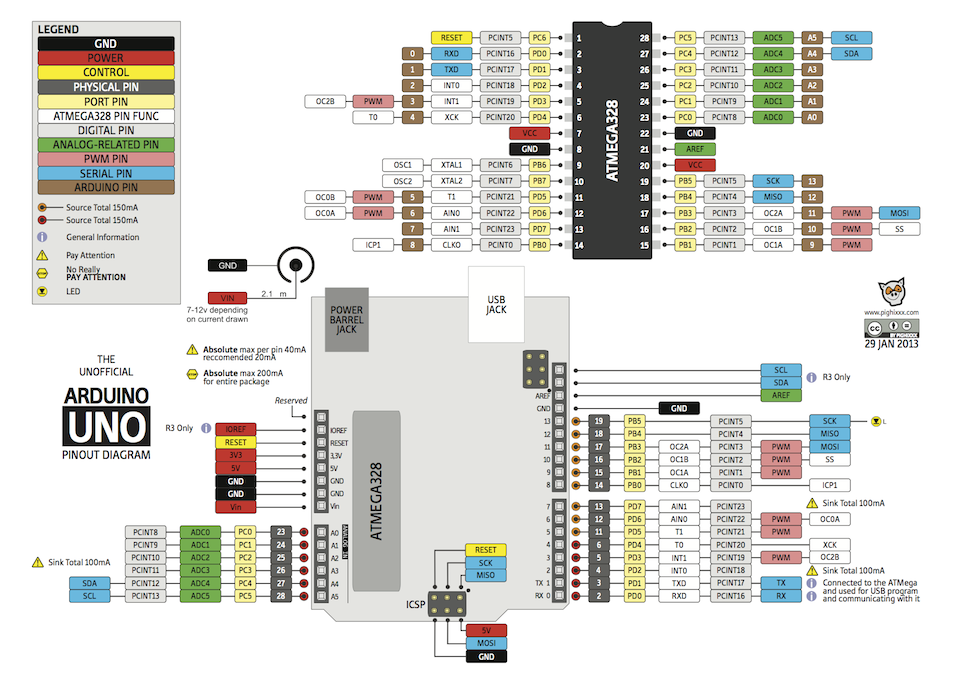
\includegraphics[width=\textwidth]{figuras/Arduino-Uno-Pinout}
	\caption{Pinagem do Arduino Uno}
	\label{fig:pinagem-arduino-uno}
\end{figure}

A linguagem de programação arduino é basicamente a linguagem C++ para microcontroladores ATMEL, mas com algumas funções e definições facilitadoras. A principal diferença entre C++ e a linguagem arduino é que não existe a função main(), mas sim as funções (ou rotinas) \lstinline|setup()| e \lstinline|loop()|. A função \lstinline|setup()| é executado apenas uma vez no momento que o arduino é ligado (ou resetado) e depois o código dentro da função \lstinline|loop()| é executado repetidamente. Com isto o esqueleto de um programa arduino fica:

\begin{lstlisting}[caption=Esqueleto de um programa arduino., label=lst:ardEsquel]
void setup() {
  //codigo a ser executado no inicio
}

void loop() {
  //codigo a ser executado repetidamente
}
 \end{lstlisting}

Lembrando que no arduino, como no C, tudo que tiver depois de \lstinline|//| é comentário e é ignorado pelo compilador.

\section{Piscando um led.}
Vamos passar logo a um exemplo para analisar um programa arduino. As placas de arduino UNO já tem um led ligado ao pino 13, identificado por um L na placa. Podemos fazer um programa que faça este led piscar.

\begin{lstlisting}[caption= Programa para piscar led.,label=lst:piscaled]
void setup() {
  //codigo a ser executado no inicio
  pinMode(13,OUTPUT); //define o pino 13 como uma saida (led)
}

void loop() {
  //codigo a ser executado repetidamente
  digitalWrite(13,LOW);  //apaga o led
  delay(500);            //espera meio segundo
  digitalWrite(13,HIGH); //acende o led
  delay(500);            //espera meio segundo
}	
\end{lstlisting}

A chamada \lstinline|pinMode(13, OUTPUT);| serve para definir que o pino 13 será uma saída. Obviamente isto só precisa ser feito no início do programa, logo está dentro de \lstinline|setup()|. Se quiséssemos ter uma entrada digital, usaríamos a mesma função, mas trocando OUTPUT por INPUT: \lstinline|pinMode(pino,INPUT);|.

A função que define o valor de um pino digital é a \lstinline|digitalWrite(pino,valor)|. Ela é chamada duas vezes no código \ref{lst:piscaled} dentro de \lstinline|loop()|, uma para apagar o led (gravando \lstinline|LOW|) e outra para acendê-lo (gravando \lstinline|HIGH|). \lstinline|LOW| e \lstinline|HIGH| são duas constantes, de valor 0 e 1, referentes ao zero e um lógico, respectivamente. Na prática, no sistema arduino, o \lstinline|LOW| é uma tensão próxima a \SI{0}{V} e o \lstinline|HIGH| uma tensão próxima a \SI{5}{V}.

Um detalhe é que o microcontrolador do arduino funciona numa velocidade de 8 ou \SI{16}{MHz} (dependendo da versão), logo se colocássemos apenas as duas chamadas à função \lstinline|digitalWrite| não veríamos o led piscar, mas teríamos a impressão que ele está aceso com metade da intensidade. Para vermos o led piscar é necessário colocar um atraso, que é justamente obtido pela função \lstinline|delay(x)|, que gera um tempo morto de \lstinline|x| milisegundos.

Se quiséssemos saber o valor de um pino digital que tivesse sido definido como entrada, a função seria \lstinline|digitalRead(pino)|, que retornaria o valor digital naquele pino. Pode-se usar isto por exemplo, para fazer com que uma saída digital seja a cópia de uma entrada digital, como no código \ref{lst:ardCopiaDig}.
\begin{lstlisting}[caption= Programa para acender um led em função de uma entrada digital.,label=lst:ardCopiaDig]
const int pinoSaida = 13;
const int pinoEntrada = 10;

int valor;

void setup() {
  //codigo a ser executado no inicio
  pinMode(pinoSaida,OUTPUT); //define a saida (led)
  pinMode(pinoEntrada,INPUT); //define a entrada
}

void loop() {
  //codigo a ser executado repetidamente
  valor = digitalRead(pinoEntrada); //le a entrada
  digitalWrite(pinoSaida,valor);  //e escreve na saida
}	
\end{lstlisting}

No código \ref{lst:ardCopiaDig} acrescentamos também algumas variáveis. Duas são constantes com os pinos usados. Elas facilitam a leitura do código e também facilitam caso posteriormente quisermos mudar os pinos utilizados. A outra variável armazena o valor lido da entrada, que depois é escrito na saída. 

%Altere o código do seu programa para que ele faça piscar um led ligado ao pino 5 do arduino.
\section{Sinais analógicos}
Em contraste com os sinais digitais, os sinais analógicos são aqueles que podem assumir qualquer valor de tensão. No contexto do arduino, vamos por enquanto assumir que os sinais analógicos estão entre \SI{0}{V} e \SI{5}{V}.

Para valores analógicos, usamos as funções \lstinline|analogWrite(pino,valor)| e \lstinline|analogRead(pino)|, que, ao contrário das equivalentes digitais, são restritas a alguns pinos específicos. As entradas analógicas são identificadas pelos pinos ANALOG IN (A0 a A5 no arduino) e são ligadas a um conversor analógico/digital (A/D) do microcontrolador, que transforma estes sinais numa palavra binária de 10 bits. Como $2^{10} = 1024$, isto significa que a função \lstinline|analogRead| retorna um valor entre 0 (para uma entrada de 0 V) e 1023 (para uma entrada de 5 V).

O arduino não tem um conversor D/A, logo a função \lstinline|analogWrite| não gera um sinal analógico verdadeiro no pino. O que esta função faz é gerar um sinal modulado por largura de pulso - PWM (\emph{Pulse Width Modulation}).

O sinal PWM é um trem de pulsos digital, com frequência da ordem de \SI{500}{Hz} (no caso do arduino) cuja razão entre o tempo em alto e o perído (conhecida como \emph{duty cycle}) pode ser alterada pelo parâmetro passado, como mostra a figura \ref{fig:pwm}.
\begin{figure}[hbt]
	\centering
	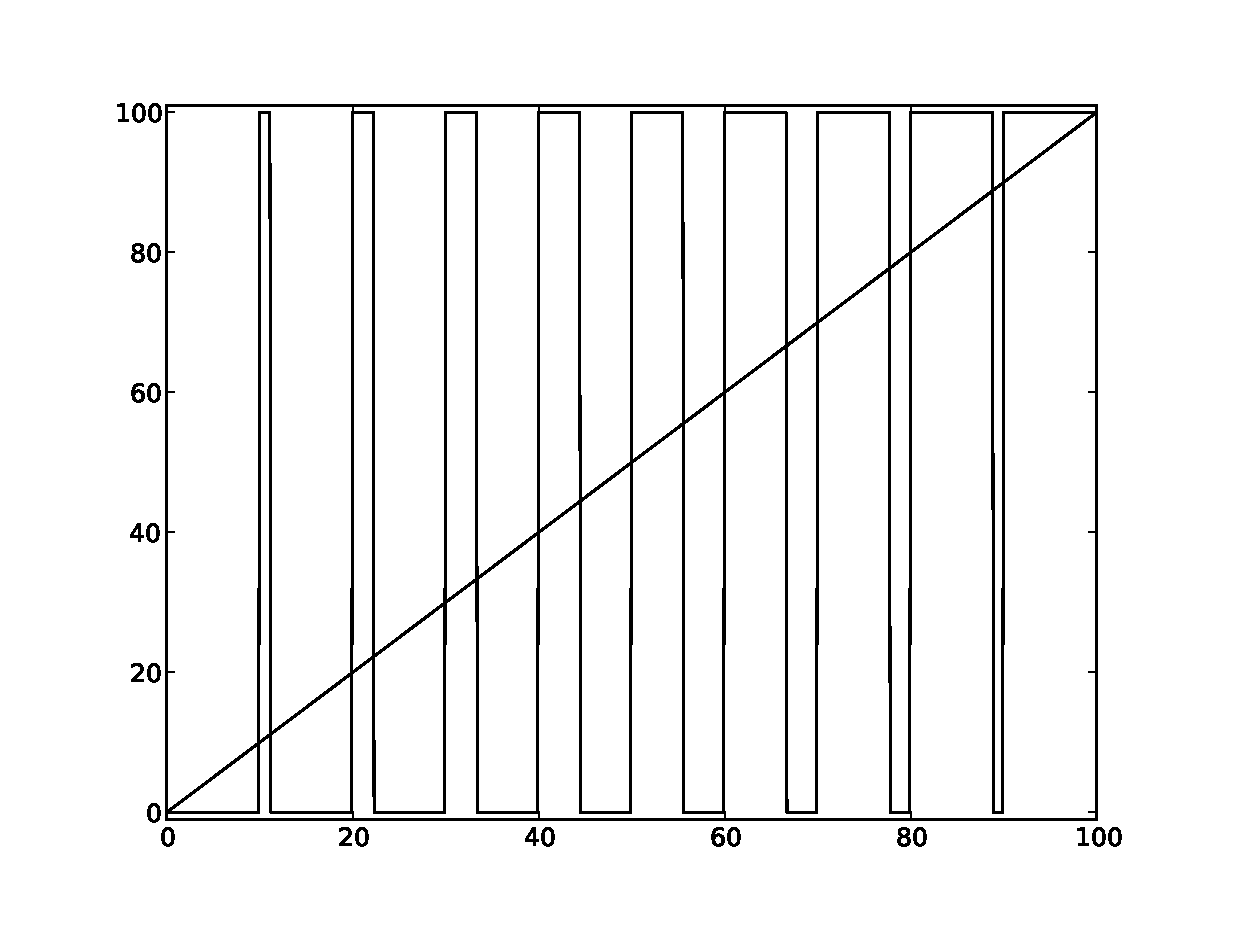
\includegraphics[width=\textwidth]{figuras/pwm}
	\caption{Reta modulada em largura de pulso (PWM).}
	\label{fig:pwm}
\end{figure}	
 Se um sinal PWM é enviado a um pino com um led, ele piscará 500 vezes por segundo, o que é muito rápido para o olho humano, de modo que na prática o que se vê quando se varia o duty cycle de um sinal PWM que aciona um led é uma variação de sua intensidade. Logo um sinal PWM funciona, para muitas aplicações, como um sinal analógico.

Novamente, não são todos os pinos do arduino que conseguem gerar este sinal PWM, logo a função \lstinline|analogWrite| está restrita aos pinos 3, 5, 6, 9, 10 e 11. Um outro detalhe que vale a pena ressaltar é que enquanto a função \lstinline|analogRead| gera um valor entre 0  1023, a \lstinline|analogWrite| recebe como parâmetro um valor entre 0 e 255 apenas.

Uma função útil do arduino para lidar com este tipo de situação é a função \lstinline|map(valor, minIn, maxIn, minOut, maxOut)|, que faz uma transformação linear de valor de acordo com a seguinte equação:
\begin{equation*}
(\text{valor} - \text{minIn}) \times \frac{\text{maxOut} - \text{minOut}}{\text{maxIn} - \text{minIn}} + \text{minOut}
\end{equation*}

A partir desta função, um código que leia o valor gerado pelo potenciômetro (em A0) e controle a intensidade do led no pino 5 poderia ser simplesmente:
\begin{lstlisting}
analogWrite(5,map(analogRead(A0),0,1024,0,256));
\end{lstlisting}

Note que o valor lido pelo \lstinline|analogRead| não precisa ser usado apenas na função \lstinline|analogWrite| mas pode ser usado para outra finalidade, como por exemplo alterar um atraso.
%Faça um programa que altere a frequência com que um led pisca em função da posição de um potênciometro.
%Repita o problema anterior, só que agora fazendo com que o led RGB ligado nos pinos 9, 10 e 11 pisque na sequencia vermelho, verde e azul, com a frequência definida pelo potenciômetro.
  
\section{Controle: for e if}
Até aqui foram feitos programas puramente sequenciais, porém em vários momentos é interessante realizar operações repetidas vezes ou realizar algumas tarefas apenas em situações específicas. Para estes casos existem comandos como o \lstinline|for| e o \lstinline|if|.
O comando for serve para tarefas repetidas. Por exemplo, se quiséssemos inicializar os pinos de 2 a 10 como saídas com valor LOW, poderíamos usar o seguinte código:
\begin{lstlisting}
for(int i = 2; i<11; i++){
	pinMode(i,OUTPUT);
	digitalWrite(i,LOW);
}	
\end{lstlisting}
O que este código faz é definir uma variável local i com valor inicial 2 depois ele checa se i é menor que 11, se for ele executa os comandos que estão entre as chaves ``\{'' e ``\}'', incrementa a variável \lstinline|i| (\lstinline|i++|) e checa novamente. Quando \lstinline|i < 11| for falso, ele sai do laço.

%Faça um programa que faça o led piscar suavemente (a intensidade variando entre apagado e totalmente aceso)
O comando if executa um determinado código apenas se determinada condição for verdadeira. Por exemplo, para acender um led apenas se um sinal analógico for maior que a metade da escala (512 = 1024/2)  pode-se escrever:
\begin{lstlisting}
if(analogRead(A0) >= 512){
	digitalWrite(13,HIGH);
}
\end{lstlisting}

Note que este código apenas fará alguma coisa se a condição for verdadeira. Para fazer uma coisa OU outra usa-se o comando \lstinline|else| após o \lstinline|if|:
\begin{lstlisting}
if(analogRead(A0) >= 512){
	digitalWrite(13,HIGH);
} else {
	digitalWrite(13,LOW);
}
\end{lstlisting}
%Faça o led rgb piscar suavemente em vermelho, azul ou verde dependendo do potenciômetro.
\section{Comunicação com o computador}
Como já dito, a conexão USB do arduino serve também para a comunicação do mesmo com o computador. Do lado do computador o arduino aparece como uma porta serial e o próprio programa contém um terminal serial pelo qual é possível se comunicar com o arduino. Do lado do arduino, os pinos 0 e 1 são os pinos transmissor e receptor ligados ao USB .

A programação é feita através do objeto  \lstinline|Serial|. Este objeto tem vários comandos, porém para nós os que interessam neste momento são:
\begin{description}
	\item[Serial.begin(baud)] Inicializa a comunicação serial na velocidade (baud rate) indicada.
	\item[Serial.read()] Retorna o valor de um byte recebido ou -1 caso não tenha sido recebido nenhum byte.
	\item[Serial.print(dado) e Serial.println(dado)] Se dado for um char ou uma string (texto), envia dado. Se dado for um número, envia este número como uma string. No caso de println, é acrescentada uma quebra de linha após dado.
	\item[Serial.available()] Retorna o número de bytes recebidos que ainda não foram lidos.
\end{description}

%Controle a intensidade das cores do led rgb pelo computador, enviando “cn” pela serial, onde 'c' é igual a 'r', 'g' ou 'b' e 'n' é um byte.

\chapter{CLPs -- Definições e termos comuns}

A IEC61131, antes conhecida por IEC1131 é uma norma técnica do \emph{International Eletrotechnical Commission}, que define um padrão para CLPs. Esta norma define vários requisitos de hardware e software para os CLPs, desde aspectos de segurança até guias de uso.

No CLP há um programa principal que executa a sequência mostrada na figura \ref{fig:seq_clp}. Em condições normais, o CLP fica num loop executando as seguintes operações:
\begin{enumerate}
  \item Lê as entradas, armazenando uma cópia das entradas em posições de memória.
  \item Executa o código programado.
  \item Atualiza as saídas, em função das entradas e do código do usuário.
  \item Se comunica com outros dispositivos, se houverem. Estes outros dispositivos podem ser: computador, outro CLP, IHM, etc.
  \item Faz um auto-teste.
\end{enumerate}

\begin{figure}[!h]
  \centering
  \begin{tikzpicture}[node distance = 2.0cm, auto]
    \tikzstyle{block} = [rectangle, draw,% fill=blue!20,
    text width=5.5em, text centered, rounded corners, minimum height=3em]
    \tikzstyle{line} = [draw, -latex']


    % Place nodes
    \node [block] (init) {Inicialização};
    \node [block, below of=init] (leitura) {Leitura das Entradas};
    \node [block, below of=leitura] (exec) {Código Programado};
    \node [block, below of=exec] (escrita) {Escrita das saídas};
    \node [block, below of=escrita] (com) {Comunicação};
    \node [block, below of=com] (teste) {Auto-teste};
    \node [block, fill=red!20, right=2cm of teste] (erro) {Falha};

    \path [line] (init) -- (leitura);
    \path [line] (leitura) -- (exec);
    \path [line] (exec) -- (escrita);
    \path [line] (escrita) -- (com);
    \path [line] (com) -- (teste);
    \path [line] (teste) --node[above]{Erro} (erro);
    \path [line] (teste) |- +(-2,-1) |- (leitura);


  \end{tikzpicture}
  \caption{Sequência do programa principal de um CLP.\label{fig:seq_clp}}
\end{figure}

A este loop se chama ciclo de execução, ciclo de \emph{scan} ou \emph{scan cycle}. O tempo que o CLP demora executando esta sequência é conhecido por \emph{scan time}. O ideal é que este tempo seja tão pequeno a ponto de poder ser desprezado em comparação aos tempos do processo. Neste contexto o código do usuário deve ser visto como tendo uma execução imediata. Obviamente isto não é verdade, já que o processador que executa este código é uma máquina de Turing -- que é inerentemente sequencial. Em processos simples, o \emph{scan time} pode ser da ordem de milissegundos ou dezenas de milissegundos, o que é bem rápido para uma grande quantidade de processos. Isto é especialmente importante quando se trabalha com a linguagem ladder, cuja estrutura remete a um circuito elétrico que é inerentemente paralelo, porém o \emph{scan time} depende do número de variáveis e do tamanho do código, podendo chegar a algumas centenas de milissegundos, onde a abstração de execução imediata pode deixar de funcionar.

Há porém, mesmo em processos simples, situações em que é necessário que o CLP atue mais rápido que no tempo do \emph{scan time}, como por exemplo na leitura de um encoder, cujo sinal pode facilmente passar de kiloHertz. Para estes casos se usa um recurso dos microprocessadores e microcontroladores chamado interrupção, que permite interromper momentaneamente a execução do programa normal para executar uma tarefa mais prioritária, como por exemplo a leitura do encoder.

Outro uso de interrupção é um recurso de segurança chamado \emph{watchdog timer}: um temporizador que é resetado uma vez a cada ciclo de execução. Se houver algum problema ou no código ou no hardware do microcontrolador que faça com que o ciclo de execução demore mais que o tempo ajustado no \emph{watchdog timer} (tipicamente da ordem de \SI{200}{\milli\second}), este causa uma interrupção que envia o CLP ao estado de Falha.

CLPs mais modernos ainda permitem um outro modo de funcionamento, que permite aplicar redundância para aumentar a robustez do sistema de controle: colocam-se 2 CLPs ligados aos mesmos módulos de entrada e saída e com o mesmo programa gravado. Os dois executam o mesmo programa, só que apenas um deles aciona as saídas. Se este falhar, o segundo assume seu lugar sem interrupção do controle. A isto se chama \emph{hot swap}.

\section{Variáveis}

As variáveis dos CLPs e de seus módulos de controle são segmentaas de acordo com seu uso. Elas podem se referenciar a um valor dos seguintes tipos: entrada (I), saída (Q), memória interna (M) ou constante (K). O formato desta variável pode ser bit (X), byte (B) palavra de 16 bits, ou \emph{word} (W), palavra de 32 bits, \emph{double word} (D), de 64 bits, \emph{long word} (L),  ou número real em ponto flutuante (F). É possível -- e aconselhável -- definir símbolos que representem as memórias utilizadas num determinado programa, mas o símbolo deve apontar para uma memória descrita da seguinte forma:
\begin{center}
\textbf{\%\{tipo\}\{formato\}\{pos\}}
\end{center}

\textbf{pos} vem de posição, que pode ser simplesmente o endereço daquela variável dentro daquele segmento. Porém, ao se ter módulos, precisa-se colocar qual módulo está sendo endereçado, o que normalmente é feito pela posição do módulo no barramento (\emph{rack}) em que está montado. Neste caso é comum o \textbf{pos} ser da forma:
\begin{center}
\textbf{\{rack\}.\{módulo\}.\{canal\}}
\end{center}

Por exemplo:

\begin{description}
  \item[\%IX100] -- Bit de memória de entrada na posição 100.
  \item[\%I100] -- Idem, pois para bit pode-se deixar o formato implícito.
  \item[\%QW122] -- Word de memória de saída na posição 122.
  \item[\%IW10.1.21] -- Word de memória de entrada no rack 10, módulo 1, canal 21.
  \item[\%IX0.1.0] -- entrada binária 0 no módulo 1.
\end{description}

Obviamente, o módulo precisa ter fisicamente aquele tipo de varíavel para ser endereçado.

\section{Programação}
O código programado é definido pelo usuário e é composto por um conjunto de blocos em 5 possíveis linguagens, descritas na norma:
\begin{description}
  \item[IL -- Instruction List] Uma linguagem de baixo nível de abstração, parecida com assembly.
  \item[ST -- Structured Text] Uma linguagem textual de alto nível, tal como C ou Pascal.
  \item[LD -- Ladder] Baseado no diagrama de circuitos a relê.
  \item[FBD -- Function Block Diagram] Parecido com um diagrama de portas lógicas: blocos com entradas e saídas.
  \item[SFC -- Sequential Function Chart] Baseado em Grafcet, uma extensão de máquina de estados.
\end{description}

Os blocos podem ser independentes, e neste caso eles são executados um após o outro na sequência em que estão na memória, ou podem haver blocos de subrotinas, que são executados quando chamados por outro bloco. É possível ter um bloco de uma linguagem chamando blocos de outras linguagens, o que aumenta bastante o poder descritivo destas linguagens. Além disso as variáveis são geralmente globais e acessíveis de todos os blocos, em qualquer linguagem.

Na prática, a maior parte da programação de um CLP é feita em Ladder, pois é a linguagem mais conhecidas pelos técnicos, responsáveis primeiros da manutenção dos equipamentos. Há também um grande uso de SFC devido a facilidade de usar esta linguagem para resolver problemas sequenciais. Além disso, o Grafcet (no qual é baseado o SFC) pode ser usado como uma ferramenta de desenvolvimento de um programa em ladder. Por conta disto este texto tratará principalmente destas duas linguagens. Porém antes será feita uma breve análise de Ladder e Instruction List, pois permite termos uma melhor ideia de como é o funcionamento interno de um CLP.

%!TEX root = principal.tex
\section{Ladder como uma linguagem}

Apesar de parecer com um circuito, um diagrama ladder é a descrição de um código, executado da esquerda para a direita e de cima para baixo. Na prática, o ladder tem uma estrutura muti parecida com o Instruction List, portanto é interessante compararmos os 2.

Para o funcionamento do ladder ou de IL, o CLP trabalha com uma estrutura chamada pilha, que é uma memória do tipo LIFO -- \emph{last in, first out}, que pode ser visualizada como uma pilha de papel, onde o último papel colocado é o primeiro retirado. A pilha tem duas funções básicas de acesso: a load (LD), que carrega um dado de alguma posição de memória para o topo da pilha, e a store (ST), que armazena a informação no topo da pilha em alguma posição de memória. Estas posições de memória podem ser memórias internas, entradas ou saídas de um CLP. Pos simplicidade, chamemos o topo da pilha de acumulador.

Na linguagem IL, as instruções lidam diretamente com o acumulador, que passa a funcionar como uma variável implícita. Por exemplo: um código IL que define uma saída como o E de duas entradas é simplesmente:
\begin{lstlisting}[caption=Código IL de um E lógico, label=lst:andIL]
LD %I0
AND %I1
ST %Q0
\end{lstlisting}

No código \ref{lst:andIL}, a instrução \lstinline|LD %I0| carrega a entrada 0 no acumulador. Logo depois a instrução \lstinline|AND %I1| faz o E lógico do valor na entrada 1 com o valor no acumulador (que foi copiado da entrada 0) e guarda o resultado no próprio acumulador. É como se retirasse o valor da pilha, fizesse a operação, e guardasse de volta na pilha. Agora o acumulador contém o resultado do E lógico entre \lstinline|%I0| e \lstinline|%I1|. Por último, a instrução \lstinline|ST %Q0| passa o valor no acumulador para a saída 0.

Este código é equivalente ao ladder da figura \ref{fig:ladder_AND}. Neste caso, o primeiro contato carrega a entrada 0 no acumulador. Como o segundo contato está em série, ele equivale à AND do IL. A bobina então salva o valor presente no acumulador na saída 0. Note-se então a relação que há entre a bobina do ladder e o comando ST do IL e entre o contato do ladder e os comandos LD, AND e OR do IL. Não é então de se admirar que se tenha o equivalente aos contatos normalmente fechados em IL -- basta acrescentar um N aos comandos IL: LDN, STN, ANDN, ORN.

\begin{figure}[hbt]
	\centering
	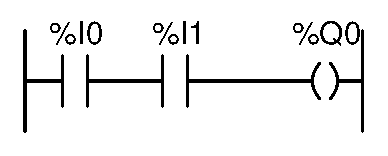
\includegraphics[scale=0.6]{figuras/ladder_AND}
	\caption{Ladder equivalente ao IL do código \ref{lst:andIL}.}
	\label{fig:ladder_AND}
\end{figure}

A pilha acaba sendo usada quando se tem caminhos paralelos no ladder. Analise-se por exemplo o ladder da figura \ref{fig:ladder_ABorCD}. Um compilador ladder, analisando o diagrama da esquerda para a direita, vai carregar A, fazer o AND com B e, chegando à junção, checar de onde ela se origina, ele então vai carregar C, no topo da pilha acima do resultado do AND entre A e B que já está lá, fazer o AND com D, então fazer o OR entre os dois valores no topo da pilha e salvar o resultado em X. Um código IL equivalente é mostrado ao lado do ladder. Observe no IL que neste caso o comando OR não tem nenhum argumento; o que faz com que ele execute a operação com os dois últimos valores da pilha.

\newsavebox\ladderABorCD
\begin{lrbox}{\ladderABorCD}
\begin{minipage}[b]{0.3\textwidth}
\begin{lstlisting}
LD A
AND B
LD C
AND D
OR
ST X
\end{lstlisting}
\end{minipage}
\end{lrbox}

\begin{figure}[hbt]
	\centering
	\subfloat[ladder]{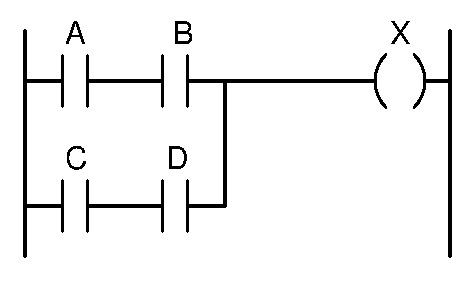
\includegraphics[scale=0.6]{figuras/ladder_ABorCD}}
	\qquad\qquad
	\subfloat[IL]{\centering\usebox{\ladderABorCD}
	}
	\caption{Exemplo de ladder e IL que usa a pilha para armazenar um valor intermediário.}
	\label{fig:ladder_ABorCD}
\end{figure}


\section{Memória}
É possível no ladder, assim como também o é usando relês, acionar uma bobina X com uma lógica que usa o contato X. Isto gera uma realimentação que tem umas propriedades interessantes. Veja por exemplo o ladder e equivalente IL da figura \ref{fig:ladder_latch}.

\newsavebox\mybox
\begin{lrbox}{\mybox}
\begin{minipage}[b]{0.3\textwidth}
\begin{lstlisting}[]
LD %I0
OR %M0
ANDN %I1
ST %M0
\end{lstlisting}
\end{minipage}
\end{lrbox}


\begin{figure}[hbt]
	\centering
	\subfloat[ladder]{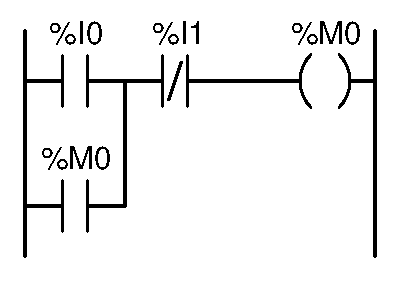
\includegraphics[scale=0.6]{figuras/ladder_latch}}
	\qquad\qquad
	\subfloat[IL]{\centering\usebox{\mybox}
	}
	\caption{Ladder e IL implementando um latch.}
	\label{fig:ladder_latch}
\end{figure}

Esta estrura faz com que, se \%I0 for acionado, aciona-se \%M0, que fica acionado daí por diante independente de \%I0. \%M0 só deixa de ser acionado se for acionado \%I1. Isto faz com que \%M0 implemente uma memória de 1 bit. Esta estrutura é a base inicial das primeiras memórias de computadores eletromecânicos e é chamada de latch. Neste caso \%I0 funciona como o sinal de SET e \%I1 como o reset deste latch.

Por ser muito útil, a funcionalidade de latch acaba sendo criado diretamente, pelos comandos de set (S em IL e 
\includegraphics[height=0.9em]{figuras/bobina_S} em ladder) e reset, (R em IL e 
\includegraphics[height=0.9em]{figuras/bobina_R} em ladder). Estes comandos fazem com que o exemplo da figura \ref{fig:ladder_latch} possa ser implementado mais facilmente, como mostra a figura \ref{fig:ladder_latchSR}.
\newsavebox\latchSRbox
\begin{lrbox}{\latchSRbox}
\begin{minipage}[b]{0.3\textwidth}
%\vspace{0pt}
\begin{lstlisting}[]
LD %I0
S %M0
LD %I1
R %M0
\end{lstlisting}
\end{minipage}
\end{lrbox}


\begin{figure}[hbt]
	\centering
	\subfloat[t][ladder]{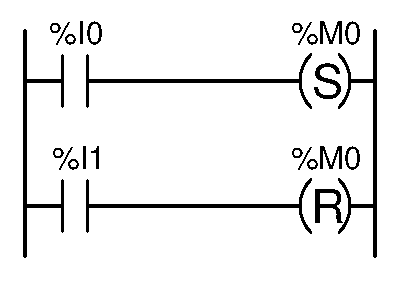
\includegraphics[scale=0.6]{figuras/ladder_latchSR}}
	\qquad\qquad
	\subfloat[t][IL]{\centering\usebox{\latchSRbox}
	}
	\caption{Ladder e IL implementando um latch com os comandos de set e reset.}
	\label{fig:ladder_latchSR}
\end{figure}

\subsection{Subida e descida de uma entrada.}

Considere que se queira inverter uma saída cada vez que se aperte um botão. A princípio bastaria fazer o ladder da figura \ref{fig:ladder_pulsoRuim}, que ao apertar o botão, seta a saída se ela estiver 0 ou reseta se estiver 1. Porém esta solução não funciona, pois a cada ciclo a situação da saída estará trocada e ela vai acabar oscilando enquanto a chave estiver pressionada.

\begin{figure}[hbt]
	\centering
	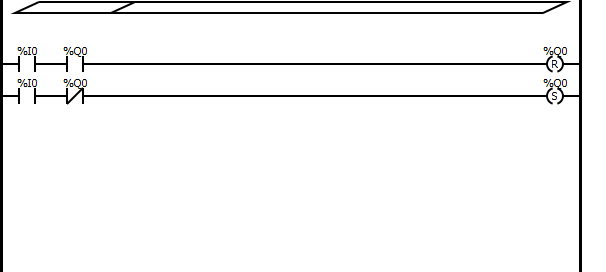
\includegraphics[width=\textwidth]{figuras/pulsoRuim}
	\caption{Troca de saída ao apertar um botão -- solução errada.}
	\label{fig:ladder_pulsoRuim}
\end{figure}

É necessário então um modo de garantir a inversão da saída apenas da primeira vez que se detecta o botão apertado. Isto pode ser conseguindo armazenando o botão numa variável auxiliar \emph{apenas ao final} do ciclo. Deste modo a variável auxiliar vai armazenar a entrada \emph{antiga}, do ciclo anterior. Com isto podemos detectar a subida da entrada se a entrada estiver acionada mas sua cópia antiga não estiver. Isto é feito na figura \ref{fig:ladder_pulso}.
\begin{figure}[hbt]
	\centering
	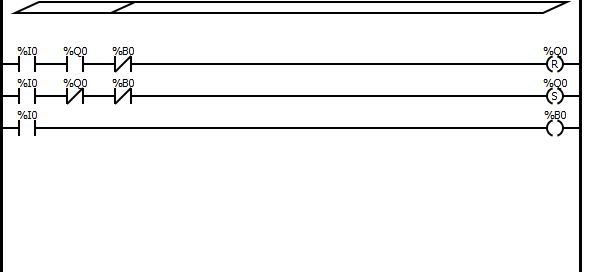
\includegraphics[width=\textwidth]{figuras/pulso}
	\caption{Troca de saída ao apertar um botão -- solução correta.}
	\label{fig:ladder_pulso}
\end{figure}

A norma define um comando específico para ladder nesta situação, que é acionado apenas no primeiro ciclo que a variável é acionada. Este comando é identificado por um contato com um P no meio, muito embora o classicladder use um chapeuzinho, identificando a subida do sinal. Também há um comando específico para determinar a descida de um sinal, indicado ou por um N no meio do contato ou por um chapeuzinho descendo, no caso do classicladder.

\begin{figure}[hbt]
	\centering
	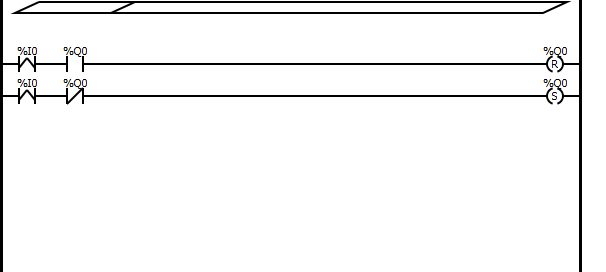
\includegraphics[width=\textwidth]{figuras/pulso2}
	\caption{Troca de saída ao apertar um botão usando o detetor de subida.}
	\label{fig:ladder_pulso2}
\end{figure}

\section{Temporizadores}

\section{Contadores}
%!TEX root = principal.tex
\section{Contadores}

Contadores crescentes e decrescentes. Tem o nome \%Cxx e conta com dois valores numéricos: \%Cxx.V, o valor de contagem e \%Cxx.P, o valor de preset. Na implementação do classicladder, o contador pode contar de 0 a 9999. O contador tem as seguintes entradas que modificam o valor de contagem V:
\begin{description}
	\item[R -- reset] leva o contador para 0 quando acionado.
	\item[P -- preset] leva o contador para o valor de preset quando acionado.
	\item[U -- up] incrementa o contador na subida.
	\item[D -- down] decrementa o contador na subida.
\end{description}

O contador tem as seguintes saídas:
\begin{description}
	\item[D -- done] acionado quando a contagem alcança o valor de preset (\%Cxx.V = \%Cxx.P).
	\item[E -- empty] acionado quando o contador está em zero e é decrementado (V vai para 9999). Também chamado de underflow.
	\item[F -- overflow] acionado quando o contador está em 9999 e é incrementado (V vai para 0).
\end{description}

As saídas também são disponíveis como variáveis, no formato \%Cxx.X, onde xx é o número do contador e X a variável (V, P, D, E ou F). O limite de contagem pode ser resolvido com o uso destas variáveis. Por exemplo, pode-se fazer um contador que conta até 34357 da forma mostrada na figura \ref{fig:cl_grande_contador}.
\begin{figure}[hbt]
	\centering
	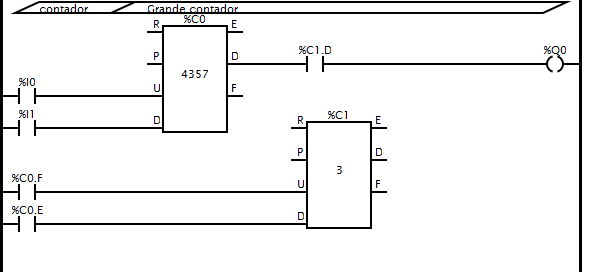
\includegraphics[width=\textwidth]{figuras/cl_grande_contador}
	\caption{Contador com preset de 34357 feito com dois contadores.}
	\label{fig:cl_grande_contador}
\end{figure}

\subsection{Acesso às variáveis}

As variáveis do contador, assim como outras variáveis numéricas, podem ser lidas ou definidas usando os blocos COMPARE ou OPERATE.

O bloco COMPARE retorna um valor booleano (acionado ou não acionado) definido por uma expressão matemática. Esta expressao pode conter:
\begin{itemize}
\item variáveis numéricas: \%W0, \%W3 ou símbolos definidos;
\item operadores matemáticos padrões, $+$, $-$, $*$, $/$, \^{} (potência), \% (módulo);
\item comparações, =, <, >, <=, >=, <> (diferente);
\item operadores lógicos, $\&$ (and), $|$ (or);
\item Funções: ABS (valor absoluta de um valor), MOY (média, em francês)/AVG (média de valores, separados por vírgula).
\end{itemize}

O bloco OPERATE é posicionado como uma bobina e recebe uma equação da forma: <variável>=valor. Se acionado acionada, como uma bobina, faz com que a variável receba o valor descrito.

Pode-se, por exemplo, definir que, quando o contador 2 contar 5, o seu valor de preset mude para 12, como mostra a figura \ref{fig:cl_contador_variaveis}.
\begin{figure}[hbt]
	\centering
	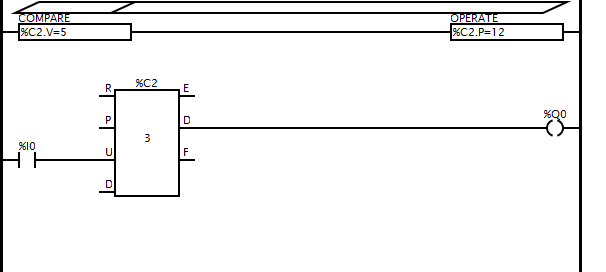
\includegraphics[width=\textwidth]{figuras/cl_contador_variaveis}
	\caption{Contador tendo seu valor de preset mudado por um bloco OPERATE.}
	\label{fig:cl_contador_variaveis}
\end{figure}

\section{Temporizadores (timers)}
O timer definido no padrão IEC61131, seguido pelo classicladder, pode ser de 3 tipos: TON, TOF ou TP. A figura \ref{fig:cl_timers} mostra um exemplo de cada um destes tipos.
\begin{figure}[hbt]
	\centering
	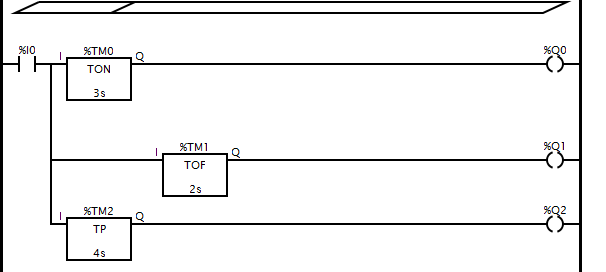
\includegraphics[width=\textwidth]{figuras/cl_timers}
	\caption{Timers TON, TOFF e TP.}
	\label{fig:cl_timers}
\end{figure}

O temporizador tipo TON causa um atraso no tempo de subida do sinal. O TOF causa um atraso no tempo de descida do sinal. O TP causa um pulso do tempo determinado iniciado pela subida do sinal de entrada. Isto pode ser visto na figura \ref{fig:tempoTimers}.
\begin{figure}[hbt]
	\centering
	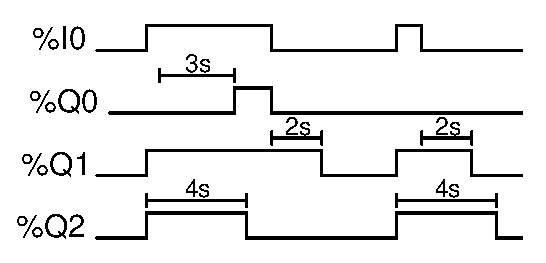
\includegraphics[scale=0.6]{figuras/tempoTimers}
	\caption{Diagrama temporal com os sinais em relação ao ladder da figura \ref{fig:cl_timers}.}
	\label{fig:tempoTimers}
\end{figure}
%!TEX root = principal.tex
\section{plcLib}

A biblioteca plcLib (http://www.electronics-micros.com/software-hardware/plclib-arduino/) define um conjunto de funções muito parecidas com as da linguagem \emph{Instruction List}, e que podem ser facilmente transcritas para a linguagem Ladder. Na configuração padrão, chamada pela função \lstinline|setupPLC()| este sistema define 4 entradas (X0 a X3, usando A0 a A3) e quatro saídas (Y0 a Y3, usando 3, 5, 6 e 9).

Usando o Multi-function Shield, as entradas correspondem ao potenciômetro (A0) e aos 3 botões, logo estão bem adequadas. As saídas correspondem ao buzzer (3) e a três conectores de servo, porém não temos nenhuma saída ligada aos leds. Para definir todas entradas e saídas de uma vez, fazemos:
\begin{lstlisting}[caption=Definição de função e constantes para usar o o Multi-function Shield com o plcLib., label=lst:setupShield]
// Definicao das constantes dos pinos
const int VR = A0;
const int S1 = A1;
const int S2 = A2;
const int S3 = A3;
const int D1 = 13;
const int D2 = 12;
const int D3 = 11;
const int D4 = 10;
const int LS1 = 3;
const int Q1 = 5; 
const int Q2 = 6; 
const int Q3 = 9; 
const int Q4 = A5; 
 
void setupShield(){ // Funcao para inicializar
   pinMode(VR,INPUT);
   pinMode(S1,INPUT);
   pinMode(S2,INPUT);
   pinMode(S3,INPUT);
   pinMode(D1, OUTPUT);
   pinMode(D2, OUTPUT);
   pinMode(D3, OUTPUT);
   pinMode(D4, OUTPUT);
   pinMode(Q1, OUTPUT);
   pinMode(Q2, OUTPUT);
   pinMode(Q3, OUTPUT);
   pinMode(Q4, OUTPUT);
   pinMode(LS1, OUTPUT);
   // Valores iniciais para apagar os leds e nao soar a buzina
   digitalWrite(D1,HIGH); 
   digitalWrite(D2,HIGH);
   digitalWrite(D3,HIGH);
   digitalWrite(D4,HIGH);
   digitalWrite(LS1,HIGH);
}
\end{lstlisting}

Deste modo basta chamarmos \lstinline|setupShield()| no setup que configuramos nossa entradas e saídas.

\subsection{Acumulador}
Os CLPs trabalham com o conceito de acumulador (que na implementação do plcLib tem o nome scanValue), que é uma variável implícita. As funções pegam implicitamente o valor a ser trabalhado do acumulador e salvam o resultado de volta nele.
O plcLib define  as funções \lstinline|in(entrada)|, \lstinline|inNot(entrada)|, \lstinline|out(saida)| e \lstinline|outNot(saida)|, equivalentes às LD, LDN, ST e STN, de Instruction List, respectivamente. As duas primeiras pegam o valor de uma entrada e guardam no acumulador, enquanto que as 2 últimas pegam o valor do acumulador e colocam na saída. O Not (N) no final indica que estes valores são invertidos.
Vejamos como exemplo o código \ref{lst:inOut}:
\begin{lstlisting}[caption=Código simples de leitura de cópia de entradas para saídas., label=lst:inOut]
void loop() {
  in(S1);      // Le chave 1
  out(D1);     // manda para led 1

  inNot(S2);   // Le chave 2 (invertida)
  out(D2);     // manda para led 2
  
  inNot(S3);   // Le chave 3 (invertida)
  outNot(D3);  // manda para led 2 (invertido)
}
\end{lstlisting}

Neste caso, D1 fica sendo uma cópia de S1, D2 o valor invertido de S2. Dá para imaginar o que acontece com D3.

É bom lembrar que no multi-function shield as chaves são conectadas ao terra, enquanto que os leds são conectados à 5V. Isto faz com que quando apertada, a chave gere um 0 lógico (não um 1) e que o led acende quando se envia um 0 lógico (e não um 1). Por isto é interessante para trabalharmos com este shield fazermos inNot(Sn), que resulta em 1 se a chave estiver apertada, e outNot(Ln), que acende o led quando o valor no acumulador for 1.

\subsection{Funções lógicas}
Mas apenas carregar um único valor não é tão interessante. Bem mais útil é montar uma relação lógica entre valores. Para isto servem as funções andBit, orBit, xorBit, andNotBit e orNotBit. Cada uma desta funções faz uma operação lógica entre o acumulador e a variável indicada, salvando o resultado no acumulador. A tabela \ref{tab:logicas} mostra as tabelas verdades de cada uma delas.

\begin{table}[h]
\caption{Tabela verdade das funções lógicas definidas em plcLib.}\label{tab:logicas}
\centering
\begin{tabular}{|cc|ccccc|}
%\usepackage{multirow}
\hline
\multirow{2}{*}{scanValue} & \multirow{2}{*}{ent} & \multicolumn{5}{|c|}{scanValue (após operação)} \\
%\cline{3-7}
 &  & andBit & orBit & xorBit & andNotBit & orNotBit\\
 \hline
0 & 0 & 0 & 0 & 0 & 0 & 1\\
0 & 1 & 0 & 1 & 1 & 0 & 0\\
1 & 0 & 0 & 1 & 1 & 1 & 1\\
1 & 1 & 1 & 1 & 0 & 0 & 1\\
\hline
\end{tabular}
\end{table}

Colocando estas funções em cascata é possível criar lógicas bem interessantes, como por exemplo, soar o alarme se S1 ou S2 forem pressionados ao mesmo tempo que S3 for pressionado.
\begin{lstlisting}[caption=Aciona a buzina em função das chaves., label=lst:buzina]
  inNot(S1);   // Le se chave 1 apertada
  orNotBit(S2);   // Le se chave 2 apertada e faz um OU logico
  andNotBit(S3);  // Le se chave 3 apertada e faz um E logico
  outNot(LS1);  // Se condicao satisfeita, aciona a buzina
\end{lstlisting}

O problema do uso do acumulador é que às vezes uma situação exige uma lógica mais complexa do que o acumulador permite. Por exemplo: como acender D2 se a maioria dos botões estiver pressionado? (Problema do voto majoritário)
Existem 2 formas de resolver este problema: pilha ou variáveis;

A pilha é como a maioria dos CLPs trabalham: ao invés de ter um único acumulador, ele tem um número finito de posições de memória que ele usa e todo comando usa implicitamente o topo da pilha. No caso da implementação do plcLib, a pilha pode ser definida separadamente como um objeto da classe Stack. Logo, se fizermos Stack pilha; definimos uma pilha de nome pilha.

Os principais comandos de acesso à pilha são o \lstinline|push()|, que passam o valor do acumulador para o topo da pilha, e o \lstinline|pop()|, que tira o valor do topo da pilha e passa para o acumulador. Outros comandos úteis para a lógica são o \lstinline|andBlock()|, que faz o E do valor no topo da pilha com o acumulador, slavando no acumulador e o \lstinline|orBlock()|, que faz a mesma coisa com o OU lógico. Usando a pilha é possível resolver o problema da maioria dos botões da seguinte forma:

\begin{lstlisting}[caption=Solução do voto majoritário com uso de pilha., label=lst:majPilha]
void loop(){\lstinline|
	inNot(S1);
	andNotBit(S2);
	andBit(S3);
	pilha.push();
	inNot(S1);
	andBit(S2);
	andNotBit(S3);
	pilha.push();
	in(S1);
	andNotBit(S2);
	andNotBit(S3);
	pilha.push();
	inNot(S1);
	andNotBit(S2);
	andNotBit(S3);
	pilha.orBlock();
	pilha.orBlock();
	pilha.orBlock();
	outNot(D2);
}
\end{lstlisting}

Outra possibilidade é simplesmente definir variáveis auxiliares para receberem os valores intermediários. Neste caso as variáveis precisam ser do tipo \lstinline|unsigned int|.
\begin{lstlisting}[caption=Solução do voto majoritário com uso de variável., label=lst:majVar]
int temp1;
void loop(){
	inNot(S1);
	andNotBit(S2);
	andBit(S3);
	out(temp1);
	inNot(S1);
	andBit(S2);
	andNotBit(S3);
	orBit(temp1);
	out(temp1);
	in(S1);
	andNotBit(S2);
	andNotBit(S3);
	orBit(temp1);
	out(temp1);
	inNot(S1);
	andNotBit(S2);
	andNotBit(S3);
	pilha.orBlock();
	pilha.orBlock();
	pilha.orBlock();
	orBit(temp1);
	outNot(D1);
}
\end{lstlisting}

Note-se que não se usou a melhor estratégia lógica para ambas soluções apresentadas. Fica como exercício resolver este problema de forma mais compacta.
\subsection{Memória}

Até o momento usamos apenas a chamada lógica combinacional, onde a saída depende apenas da entrada. Porém é bem comum a situação de querermos que a saída fique num determinado estado em função da sua história pregressa. 

Um exemplo simples: Como acionar LS1 apertando S1 e pará-lo apertando S2? O estado de LS1 depende então de qual foi o último botão apertado.

É possível implementar este tipo de memória a partir de lógica combinacional usando realimentação. Ou seja, devemos ler a saída do sistema como sendo entrada, o que, apesar de estranho, é perfeitamente possível. O código \ref{lst:latchComb} mostra justamente esta implementação.
\begin{lstlisting}[caption=Implementação de latch com lógica combinacional., label=lst:latchComb]
  inNot(S1);     // Se chave S1 apertada
  orNotBit(LS1);  // ou se LS1 ja esta acionado
  andBit(S2);    // mas apenas se S2 nao estiver apertada
  outNot(LS1);     // aciona LS1
\end{lstlisting}

Como esta função é bastante utilizada, ela recebeu o nome de \emph{latch} (tranca, ferrolho) e tem funções específicas, para deixar uma variável em 1 (função \lstinline|set()|) ou 0 (\lstinline|reset|) dali em diante, como mostrado no código \ref{lst:latch}.
\begin{lstlisting}[caption=Funções para uso de latch., label=lst:latch]
  inNot(S1);    // Se chave S1 apertada
  reset(LS1);     // Seta LS1 (aciona dai em diante)
  andBit(S2);   // Se S2 estiver apertada
  set(LS1);    // Reseta LS1 (desliga dai em diante)
\end{lstlisting}

\subsection{Temporizadores}
O arduino já tem uma função padrão \lstinline|delay|, que causa a paralisação da execução por um determinado tempo. O problema de delay é que ele para o programa todo, o que pode ocasionar problemas até de segurança.

Os temporizadores definidos na plcLib permitem gerarmos atrasos em sinais específicos, sem mexer nos demais. O timerOn atrasa a subida de um sinal, enquanto que o timerOff atrasa a descida de um sinal, como pode ser visto no exemplo abaixo. Outro tipo de temporizador é o timerPulse, que na subida do sinal de entrada gera um pulso por um tempo determinado. timerPulse e timerOff são bem parecidos, com a diferença que o último começa a medir o tempo a partir da descida da entrada, enquanto que o primeiro mede a partir da subida da entrada. Cada função destas recebe como parâmetro a variável (do tipo \lstinline|unsigned long|) que contará o tempo e o tempo final a ser contado. Logo para cada temporizador é necessário ter uma variável para armazenar o tempo utilizado.
\begin{lstlisting}[caption=Exemplos de uso de temporizadores., label=lst:temporizador]
unsigned long TIMER0 = 0;
unsigned long TIMER1 = 0;
unsigned long TIMEa = 0;
void loop(){
  inNot(S1);    // Se chave S1 apertada
  timerOn(TIMER0,2000); // atrasa subida por 2 segundos
  outNot(D1);
  inNot(S2);    // Se chave S2 apertada
  timerOff(TIMER1,2000); // atrasa descida por 2 segundos
  outNot(D2);
  inNot(S3);    // Se chave S3 apertada
  timerPulse(TIMERa, 2000);   // gera pulso de 2 segundos
  outNot(D3);
}
\end{lstlisting}

Um outro temporizador interessante é o timerCycle, que enquanto o acumulador for 1, gera um sinal alternado definido por 2 tempos: o tempo em alto e o tempo em baixo. Muito útil para alarmes.
\begin{lstlisting}[caption=Exemplos de uso timerCycle., label=lst:timeCycle]
unsigned long TempoLOW = 0;
unsigned long TempoHIGH = 0;
void loop(){
	inNot(S1);
	timerCycle(TempoLOW,1300,TempoHIGH,100);
	outNot(LS1);
}
\end{lstlisting}

\subsection{Contadores}
Um contador incrementa ou decrementa uma variável de acordo com o número de eventos que recebe. Na implementação do plcLib, estes eventos são subidas (ir de 0 para 1) em suas entradas.

Para os contadores, cria-se um objeto do tipo Counter, que tem um valor interno de preset presetValue, uma variável de contagem count, 4 entradas countUp, countDown, preset, clear e 2 saídas upperQ e lowerQ. As regras do contador são:
\begin{itemize}
  \item Uma subida em countUp incrementa o valor de count, se for menor que preset.
  \item Uma subida em countDown decrementa o valor de count, se for maior que 0.
  \item Uma subida em clear faz count igual a 0.
  \item Uma subida em preset faz count igual a presetValue.
  \item Se count for igual a 0, lowerQ retorna 1.
  \item se count for igual a preset, upperQ retorna 1.
\end{itemize}
\begin{lstlisting}[caption=Exemplo de uso do contador., label=lst:contador]
Counter ctr(10);           // Contador na faixa 0-10, comecando em zero
unsigned long TIMER0 = 0;  // 
unsigned long TIMER1 = 0;  // 

void loop() {
  inNot(S1);               // Se S1 apertada
  timerOn(TIMER0, 10);     // 10 ms de atraso para debounce
  ctr.countUp();           // incrementa ctr.
  inNot(S2);               // Se S2 apertada
  timerOn(TIMER1, 10);     // 10 ms de atraso para debounce
  ctr.countDown();         // decrementa ctr.
  inNot(S3);               // Se S3 apertada
  ctr.clear();             // zera o contador.
  ctr.lowerQ();            // Se zero,
  outNot(D1);
  ctr.upperQ();            // Se 10,
  outNot(D2);
}
\end{lstlisting}
É possível ainda criar um contador que inicializa no valor de preset. Tomando o exemplo do código \ref{lst:contador}, ao invés de fazer \lstinline|Counter ctr(10);|, faria-se \lstinline|Counter ctr(10,1);|
%\subsection{}
%!TEX root = principal.tex
\chapter{Linguagem grafcet}

GRAphe Fonctionnel de Commande Etape/Transition - Grafo funcional de comando etapa/transição, é um formalismo matemático tal como uma máquina de etapas. Tem origem na chamada máquina de etapas, mas com mais funcionalidades, tais como a possibilidade de ter etapas em paralelo e de ter macro-etapas.

Um diagrama grafcet é composto dos seguintes elementos: etapas, transições, ações, divergências e convergências E e divergências e convergências OU.

O básico do grafcet é a sequência etapa-transição-etapa, como mostra na figura \ref{fig:grafcetSimples}. Ela apresenta um diagrama grafcet com 3 etapas (os quadrados) e três transições (os retângulos verde e vermelhos). Etapas e transições podem estar ativas ou não. Etapas ativas são representadas com uma ficha dentro delas (vide Etapa 1 na figura), enquanto que transições ativas são em geral representadas por uma mudança de cor. Neste exemplo uma transição ativa é representada pela cor verde, enquanto uma inativa é representada pela cor vermelha.

A ativação de uma transição é diretemente relacionada a uma condição lógica associada a mesma: quando veradeiras, as ativam. Já a ativação das etapas depende da dinâmica do sistema. No exemplo da figura \ref{fig:grafcetSimples}, A Etapa 0 é uma etapa inicial (representado pela linha dupla), significando que o sistema inicia com a Etapa 0 ativa, mas não as demais. No momento mostrado na figura \ref{fig:grafcetSimples}, a Etapa 1 é que está ativa, indicado pela ficha.

\begin{figure}[hbt]
  \centering
  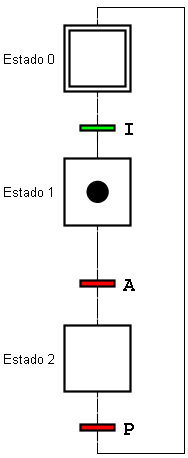
\includegraphics[scale=0.6]{figuras/grafcetSimples}
  \caption{Exemplo de um diagrama grafcet simples.}
  \label{fig:grafcetSimples}
\end{figure}

A evolução do sistema descrito em grafcet é dada pelo disparo das transições. Um transição dispara quando:
\begin{itemize}
  \item ela está ativa (ou seja, a condição ligada a ela é verdadeira) e
  \item todos as etapas anteriores a ela estão ativas.
\end{itemize}

Quando uma transição dispara ela desativa todos os etapas anteriores a ela (as etapas acima) e ativa todos as posteriores (as abaixo). Por exemplo, se na figura \ref{fig:grafcetSimples} a condição A se tornasse verdadeira, como a única etapa anterior (a Etapa 1) está ativa, esta transição dispararia, desativando a Etapa 1 e ativando a Etapa 2. Esta sequência é mostrada na figura \ref{fig:grafcetDisparo}.
\begin{figure}[hbt]
  \centering
  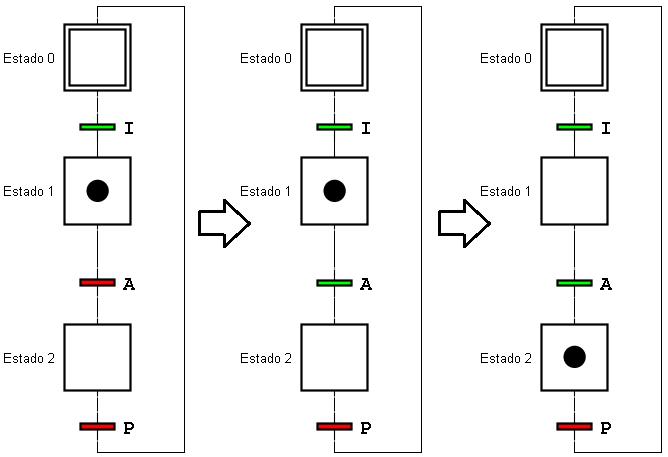
\includegraphics[scale=0.6]{figuras/grafcetDisparo}
  \caption{Sequência de disparo da transição A}
  \label{fig:grafcetDisparo}
\end{figure}

\section{Divergências e convergências}

No grafcet, pode-se ter uma etapa com mais de uma transição de saída, que pode levar para etapas diferentes de acordo com qual transição dispare primeiro. A isto se chama uma \emph{divergência OU}, pois separa em dois caminhos excludentes. Da mesma forma, duas (ou mais) transições podem levar para o mesmo etapa, o que se chama de convergência OU. A figura \ref{fig:grafcetdivOU} mostra um exemplo em que o sistema pode evoluir por dois caminhos diferentes, com o uso de divergência e convergência OU.

\begin{figure}[hbt]
  \centering
  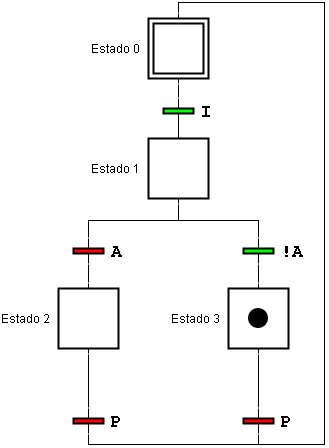
\includegraphics[scale=0.6]{figuras/grafcetdivOU}
  \caption{Exemplo de grafcet com divergência e convergência OU. O !A indica que a transição está ativa quando A for falso.}
  \label{fig:grafcetdivOU}
\end{figure}

Note-se na figura \ref{fig:grafcetdivOU} que a Etapa 1 é obrigatoriamente transitória, pois ou A é verdadeiro e o sistema evolui imediatamente para o etapa 2 ou A é falso e o sistema ativa o etapa 3. É possível definir transições que estejam ativas ao mesmo tempo, neste caso o sistema evolui para a transição com maior prioridade -- ou a mais a esquerda ou se tiver uma prioridade explícita.

Diferente de uma máquina de estados, no grafcet é permitido que uma transição acione mais que uma etapa. Neste caso o sistema se divide em caminhos paralelos. Isto é chamado de divergência E e indicado por duas linhas horizontais, para diferenciar da divergência OU. Da mesma forma, uma convergência E liga várias etapas a uma única transição, transformando caminhos paralelos num único caminho. A figura \ref{fig:grafcetdivE} mostra um exemplo de divergência e convergência E.

\begin{figure}[hbt]
  \centering
  \includegraphics[scale=0.6]{figuras/grafcetdivE}
  \caption{Exemplo de grafcet com divergência e convergência E.}
  \label{fig:grafcetdivE}
\end{figure}

Neste caso, mesmo com P ativo, o sistema não desativa a Etapa 2a nem ativa a Etapa 0, pois como a Etapa 2b não está ativa, a transição P não pode disparar.

\section{Ações}
Outra característica do grafcet é que podem ser definidas ações, ligadas a etapas. O que exatamente compõem uma ação depende da implementação do grafcet. Peguemos dois exemplos: o JGrafchart e a SFC, que é a descrição de grafcet definida pela norma IEC61131.

\subsection{JGrafchart}
\label{sub:JGrafchart}

No JGrafchart, uma ação pode ser uma definição de valor (um \emph{assignment}), da forma \lstinline|variavel = expressao|, uma chamada de subrotina (\emph{call}) ou uma variável booleana (\emph{bool}), que fica verdadeira enquanto a etapa estiver ativa. Um qualificador de uma letra define o momento em que a ação é executada:
\begin{description}
  \item[S assignment|call;] Executa apenas uma vez, quando a etapa é ativada.
  \item[X assignment|call;] Executa apenas uma vez, quando a etapa é desativada.
  \item[P assignment|call;] Executa a cada ciclo enquanto a ação estiver acionada.
  \item[N bool;] Torna verdadeira a variável booleana enquanto a etapa estiver acionada.
  \item[A assignment|call;] Executa apenas uma vez, se a etapa for desativada por uma transição de exceção (apenas definida no JGrafchart).
\end{description}

Note-se que a ação \lstinline/N bool;/ é equivalente a \lstinline/S bool=1; X bool=0;/ e é presente para facilitar a escrita, já que tal operação é feita muitas vezes.

Toda etapa tem uma variável booleana x (\lstinline|<nome_da_etapa>.x|), que é verdadeira quando a etapa é acionada, e uma variável de tempo em décimos de segundo t (\lstinline|<nome_da_etapa>.t|) e em segundos s (\lstinline|<nome_da_etapa>.s|) que contam o tempo desde que a etapa iniciou.

\subsection{SFC}
\label{sub:SFC}

As ações do SFC são do formato \textbf{\lstinline/qualificador funcao|variavel finalizado/}. \lstinline|finalizado| é uma variável opcional no caso de se usar uma função, que aciona quando a função termina, o que a torna útil para ser utilizada na transição de saída da etapa.

O qualificador pode ser qualquer um dos descritos na tabela \ref{tab:qualiSFC}. Pode-se não especificar o qualificador, onde o comportamento fica o mesmo de se usar o qualificador N. No caso da ação ser uma função, ele é executada sempre que ficar ativa. Todos os qualificadores que tem tempo acompanham um valor de tempo dado ou por uma variável ou por uma constante da forma \lstinline|T#4k|, onde k pode ser t (décimo de segundo), s (segundo), m, (minuto) ou h (hora).
\begin{table}[hbt]
  \caption{Qualificadores do SFC}
  \label{tab:qualiSFC}
  \centering

  \begin{tabularx}{\textwidth}{|c|X|}
  \hline

  \hline
  \textbf{Qualificador} & \textbf{descrição}\\
  \hline
   \textbf{N}  & Ativa a etapa estiver acionada. \\
   \textbf{S}  & Set -- ativa e mantém ativado mesmo depois de sair da etapa. \\
   \textbf{R}  & Reset -- desativa. \\
   \textbf{P}  & Ativa apenas no primeiro ciclo que a etapa estiver ativa. \\
   \textbf{L tempo}  & Ativa pelo tempo determinado enquanto a etapa estiver acionada.\\
   \textbf{SL tempo}  & Ativa pelo tempo determinado independente da etapa ainda estar acionada.\\
   \textbf{D tempo}  & Ativa após o tempo determinado enquanto a etapa estiver acionada.\\
   \textbf{SD tempo}  & Seta após o tempo determinado independente da etapa ainda estar acionada.\\
   \textbf{DS tempo}  & Seta após o tempo determinado se a etapa ainda estiver acionada.\\
  \hline

  \hline
  \end{tabularx}
\end{table}

\clearpage
\section{Níveis}
O Grafcet pode ser definido em 2 níveis de abstração: o 1 e o 2. O nível 1 serve como uma ferramenta de desenvolvimento, para analisar a partir do problema como um todo a sequência de etapas, as ações a serem realizadas em cada etapa e as condições de transição de uma etapa para outra. No nível 1 as ações e transições são descritas de forma ampla, para permitirem uma melhor visualização do processo pelo desenvolvedor. O resultado final é uma descrição dos requisitos daquelas etapas e transições e não serve como uma linguagem para programar um sistema.

Já o Grafcet nível 2 é propriamente uma linguagem de programação, com diferentes implementações. Uma delas é o SFC - \emph{Sequential Function Chart}, descrita no padrão IEC1131-3 para programação de CLPs. No SFC, cada ação corresponde a uma atuação nas saídas ou variáveis internas do CLP e cada transição corresponde a um valor binário obtido no CLP seja de entradas, seja de comparações de valores analógicos ou de tempo.

Desta forma o principal uso do grafcet é num projeto top-down, onde a partir do problema se desenvolve a sequência a ser seguida no grafcet nível 1, a partir deste se definem todas as entradas, saídas e condições necessárias para o controle automático daquela sequência e então programa-se o sistema usando grafcet nível 2.

Tomemos como exemplo uma tarefa relativamente simples: cozinhar um ovo. Considere-se o sistema da figura \ref{fig:cozinhar_ovo}, consistindo de uma panela, uma entrada de água, uma boca de fogão a gás e um mecanismo que solte o ovo na água.

\begin{figure}[!h]
\centering
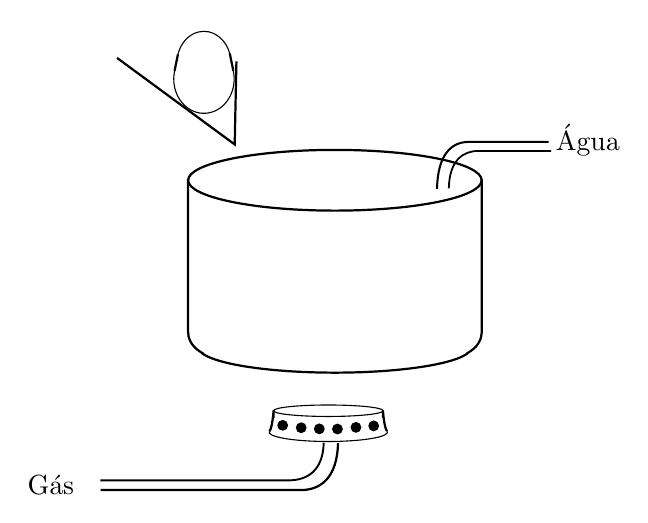
\begin{tikzpicture}[y=0.80pt, x=0.8pt,xscale=0.8,yscale=-0.8, inner sep=0pt, outer sep=0pt]
\begin{scope}[shift={(-99.03245,-288.02393)}]
    \path[draw=black,line join=miter,line cap=butt,line width=0.800pt]
      (354.2857,372.3622) .. controls (354.2857,381.8299) and (317.1893,389.5050) ..
      (271.4286,389.5050) .. controls (225.6678,389.5050) and (188.5714,381.8299) ..
      (188.5714,372.3622) .. controls (188.5714,362.8944) and (225.6678,355.2193) ..
      (271.4286,355.2193) .. controls (317.1893,355.2193) and (354.2857,362.8944) ..
      (354.2857,372.3622) -- cycle;
    \path[cm={{0.93174,0.0,0.0,0.83675,(18.52752,155.07504)}},draw=black,line
      join=miter,line cap=butt,line width=0.800pt] (351.5135,376.7594) .. controls
      (339.7757,385.9104) and (294.4050,391.3600) .. (250.1753,388.9315) .. controls
      (220.3437,387.2935) and (197.3850,382.3608) .. (190.5989,376.1313);
    \path[draw=black,line join=miter,line cap=butt,line width=0.800pt]
      (188.4845,371.6696) .. controls (188.4845,371.6696) and (188.4845,450.0421) ..
      (188.4845,457.6107) .. controls (188.4845,461.2730) and (190.0955,465.6973) ..
      (194.9956,468.8884) .. controls (198.4879,471.1627) and (197.0297,470.3066) ..
      (197.0297,470.3066);
    \path[draw=black,line join=miter,line cap=butt,line width=0.800pt]
      (354.3736,371.7266) .. controls (354.3736,371.7266) and (354.3736,450.0990) ..
      (354.3736,457.6677) .. controls (354.3736,461.3300) and (352.7625,465.7543) ..
      (347.8624,468.9454) .. controls (344.3701,471.2196) and (345.8283,470.3635) ..
      (345.8283,470.3635);
  \path[draw=black,line join=miter,line cap=butt,line width=0.800pt]
    (148.4437,303.3074) -- (214.8527,352.1376) -- (215.8294,305.2606);
  \begin{scope}[cm={{0.52126,0.0,0.0,0.55799,(132.31437,-4.68415)}}]
    \path[shift={(-3.38483,0)},draw=black] (160.1446,564.8529) .. controls
      (164.5668,583.4180) and (153.9497,602.2669) .. (136.4306,606.9532) .. controls
      (118.9114,611.6395) and (101.1244,600.3885) .. (96.7021,581.8235) .. controls
      (95.2554,575.7501) and (95.3885,569.3749) .. (97.0871,563.3753);
    \path[cm={{0.89621,0.0,0.0,-0.93321,(9.92999,1092.4228)}},draw=black]
      (160.3532,580.8939) .. controls (156.4154,599.5810) and (138.9277,611.3472) ..
      (121.2933,607.1743) .. controls (108.9462,604.2525) and (99.2953,594.0489) ..
      (96.5099,580.9713);
    \path[draw=black,line join=miter,line cap=butt,line width=0.800pt]
      (93.2329,565.0164) -- (96.8536,548.3611);
    \path[draw=black,line join=miter,line cap=butt,line width=0.800pt]
      (156.8450,565.0164) -- (153.0433,547.4560);
  \end{scope}
  \begin{scope}[shift={(0,10.0)}]
    \path[shift={(165.51847,-28.86265)},draw=black] (133.1216,521.3483) .. controls
      (133.1216,523.1376) and (119.2763,524.5880) .. (102.1973,524.5880) .. controls
      (85.1183,524.5880) and (71.2731,523.1376) .. (71.2731,521.3483) .. controls
      (71.2731,519.5591) and (85.1183,518.1086) .. (102.1973,518.1086) .. controls
      (119.2763,518.1086) and (133.1216,519.5591) .. (133.1216,521.3483) -- cycle;
    \path[cm={{0.95437,0.0,0.0,1.00307,(10.48141,-1.55578)}},draw=black]
      (304.2515,503.8934) .. controls (306.6885,506.7980) and (293.0976,509.4514) ..
      (273.8954,509.8200) .. controls (254.6932,510.1886) and (237.1512,508.1328) ..
      (234.7143,505.2283) .. controls (234.3214,504.7600) and (234.3437,504.2859) ..
      (234.7807,503.8186);
    \path[draw=black,line join=miter,line cap=butt,line width=0.800pt]
      (234.4953,503.9994) .. controls (236.1212,502.2258) and (236.7863,492.5444) ..
      (236.7863,492.5444) .. controls (236.7863,492.5444) and (236.7863,501.7823) ..
      (236.7863,492.2488);
    \path[draw=black,line join=miter,line cap=butt,line width=0.800pt]
      (300.8602,503.9994) .. controls (299.2343,502.2258) and (298.5692,492.5444) ..
      (298.5692,492.5444) .. controls (298.5692,492.5444) and (298.5692,501.7823) ..
      (298.5692,492.2488);
    \path[shift={(37.28111,-18.91723)},draw=black,fill=black] (248.7459,520.7984) ..
      controls (248.7459,522.2992) and (247.5293,523.5158) .. (246.0286,523.5158) ..
      controls (244.5278,523.5158) and (243.3112,522.2992) .. (243.3112,520.7984) ..
      controls (243.3112,519.2976) and (244.5278,518.0810) .. (246.0286,518.0810) ..
      controls (247.5293,518.0810) and (248.7459,519.2976) .. (248.7459,520.7984) --
      cycle;
    \path[shift={(26.8373,-17.9766)},draw=black,fill=black] (248.7459,520.7984) ..
      controls (248.7459,522.2992) and (247.5293,523.5158) .. (246.0286,523.5158) ..
      controls (244.5278,523.5158) and (243.3112,522.2992) .. (243.3112,520.7984) ..
      controls (243.3112,519.2976) and (244.5278,518.0810) .. (246.0286,518.0810) ..
      controls (247.5293,518.0810) and (248.7459,519.2976) .. (248.7459,520.7984) --
      cycle;
    \path[shift={(16.60251,-18.08111)},draw=black,fill=black] (248.7459,520.7984) ..
      controls (248.7459,522.2992) and (247.5293,523.5158) .. (246.0286,523.5158) ..
      controls (244.5278,523.5158) and (243.3112,522.2992) .. (243.3112,520.7984) ..
      controls (243.3112,519.2976) and (244.5278,518.0810) .. (246.0286,518.0810) ..
      controls (247.5293,518.0810) and (248.7459,519.2976) .. (248.7459,520.7984) --
      cycle;
    \path[shift={(6.36773,-18.7082)},draw=black,fill=black] (248.7459,520.7984) ..
      controls (248.7459,522.2992) and (247.5293,523.5158) .. (246.0286,523.5158) ..
      controls (244.5278,523.5158) and (243.3112,522.2992) .. (243.3112,520.7984) ..
      controls (243.3112,519.2976) and (244.5278,518.0810) .. (246.0286,518.0810) ..
      controls (247.5293,518.0810) and (248.7459,519.2976) .. (248.7459,520.7984) --
      cycle;
    \path[shift={(-4.07609,-20.0669)},draw=black,fill=black] (248.7459,520.7984) ..
      controls (248.7459,522.2992) and (247.5293,523.5158) .. (246.0286,523.5158) ..
      controls (244.5278,523.5158) and (243.3112,522.2992) .. (243.3112,520.7984) ..
      controls (243.3112,519.2976) and (244.5278,518.0810) .. (246.0286,518.0810) ..
      controls (247.5293,518.0810) and (248.7459,519.2976) .. (248.7459,520.7984) --
      cycle;
    \path[shift={(47.30687,-19.75335)},draw=black,fill=black] (248.7459,520.7984) ..
      controls (248.7459,522.2992) and (247.5293,523.5158) .. (246.0286,523.5158) ..
      controls (244.5278,523.5158) and (243.3112,522.2992) .. (243.3112,520.7984) ..
      controls (243.3112,519.2976) and (244.5278,518.0810) .. (246.0286,518.0810) ..
      controls (247.5293,518.0810) and (248.7459,519.2976) .. (248.7459,520.7984) --
      cycle;
  \end{scope}
  \path[draw=black,line join=miter,line cap=butt,line width=0.800pt]
    (273.1769,520.7233) .. controls (272.7485,540.4295) and (263.3238,547.2838) ..
    (252.1855,547.2838) .. controls (241.0472,547.2838) and (139.0890,547.2838) ..
    (139.0890,547.2838);
  \path[draw=black,line join=miter,line cap=butt,line width=0.692pt]
    (265.1049,520.6557) .. controls (264.7021,536.3302) and (255.8400,541.7823) ..
    (245.3666,541.7823) .. controls (234.8932,541.7823) and (139.0214,541.7823) ..
    (139.0214,541.7823);
  \path[fill=black] (97.967995,549.99866) node[above right] (text3077) {Gás};
  \path[draw=black,line join=miter,line cap=butt,line width=0.736pt]
    (329.0890,377.2838) .. controls (329.4517,357.5776) and (337.4309,350.7233) ..
    (346.8607,350.7233) .. controls (356.2906,350.7233) and (392.0864,350.7233) ..
    (392.0864,350.7233);
  \path[draw=black,line join=miter,line cap=butt,line width=0.638pt]
    (335.7362,376.9255) .. controls (336.0789,361.2509) and (343.6164,355.7989) ..
    (352.5243,355.7989) .. controls (361.4323,355.7989) and (393.4609,355.7989) ..
    (393.4609,355.7989);
  \path[fill=black] (396.19095,358.56888) node[above right] (text3085) {Água};
\end{scope}

\end{tikzpicture}
\caption{Sistema para cozinhar ovo sem sensores ou atuadores.}
\label{fig:cozinhar_ovo}
\end{figure}

Podemos inicialmente fazer um grafcet considerando que tudo dá sempre certo: ao iniciarmos o sistema, a panela enche de água, o ovo é colocado, o fogo acendido e aguarda-se até o ovo ficar pronto, de onde se retira a panela para tirar o ovo. Esta sequência é descrita pelo grafcet da figura \ref{fig:grafcetOvoOK}.

\begin{figure}[!h]
\centering
\includegraphics[scale=1]{figuras/ovoOK}
\caption{Diagrama grafcet nível 1 para cozinhar um ovo de forma otimista.}
\label{fig:grafcetOvoOK}
\end{figure}

Porém, problemas acontecem. Pode-se, por exemplo, esquecer de colocar a panela de volta antes de iniciar, faltar fogo ou acabar o ovo. Colocando todas estas condições a mais e defininindo o que fazer se elas acontecerem o grafcet cresce para o apresentado na figura \ref{fig:grafcetOvo1}.

\begin{figure}[!h]
\centering
\includegraphics[scale=1]{figuras/ovoNivel1}

\caption{Diagrama grafcet nível 1 para cozinhar um ovo.}
\label{fig:grafcetOvo1}
\end{figure}

Com base neste diagrama, pode-se analisar agora quais são os sensores e atuadores necessários para esta tarefa, mostrados na figura \ref{fig:cozinhar_ovo2}. São eles:

\begin{description}
  \item[S\_PP] Sensor de presença para detectar a panela.
  \item[S\_N] Sensor de distância para obter o nível de água.
  \item[S\_G] Sensor de gás.
  \item[B\_I] Botão de início.
  \item[B\_OK] Botão de OK, para continuar se der bronca.
  \item[B\_C] Botão de cancelamento.
  \item[PO] Solenóide para abrir a portinhola do ovo.
  \item[VA] Válvula de controle da água.
  \item[VG] Válvula de controle do gás.
  \item[CENTELHA] para ligar o fogo.
  \item[ALARME] para indicar que deu errado.
\end{description}

\begin{figure}[!h]
\centering
\definecolor{c0000ff}{RGB}{0,0,255}
\begin{tikzpicture}[y=0.80pt, x=0.8pt,yscale=-0.8, xscale=0.8, inner sep=0pt, outer sep=0pt]
\begin{scope}[shift={(-99.03245,-288.02393)}]
    \path[draw=black,line join=miter,line cap=butt,line width=0.800pt]
      (354.2857,372.3622) .. controls (354.2857,381.8299) and (317.1893,389.5050) ..
      (271.4286,389.5050) .. controls (225.6678,389.5050) and (188.5714,381.8299) ..
      (188.5714,372.3622) .. controls (188.5714,362.8944) and (225.6678,355.2193) ..
      (271.4286,355.2193) .. controls (317.1893,355.2193) and (354.2857,362.8944) ..
      (354.2857,372.3622) -- cycle;
    \path[cm={{0.93174,0.0,0.0,0.83675,(18.52752,155.07504)}},draw=black,line
      join=miter,line cap=butt,line width=0.800pt] (351.5135,376.7594) .. controls
      (339.7757,385.9104) and (294.4050,391.3600) .. (250.1753,388.9315) .. controls
      (220.3437,387.2935) and (197.3850,382.3608) .. (190.5989,376.1313);
    \path[draw=black,line join=miter,line cap=butt,line width=0.800pt]
      (188.4845,371.6696) .. controls (188.4845,371.6696) and (188.4845,450.0421) ..
      (188.4845,457.6107) .. controls (188.4845,461.2730) and (190.0955,465.6973) ..
      (194.9956,468.8884) .. controls (198.4879,471.1627) and (197.0297,470.3066) ..
      (197.0297,470.3066);
    \path[draw=black,line join=miter,line cap=butt,line width=0.800pt]
      (354.3736,371.7266) .. controls (354.3736,371.7266) and (354.3736,450.0990) ..
      (354.3736,457.6677) .. controls (354.3736,461.3300) and (352.7625,465.7543) ..
      (347.8624,468.9454) .. controls (344.3701,471.2196) and (345.8283,470.3635) ..
      (345.8283,470.3635);
  \path[draw=black,line join=miter,line cap=butt,line width=0.800pt]
    (148.4437,303.3074) -- (214.8527,352.1376) -- (215.8294,305.2606);
  \begin{scope}[cm={{0.52126,0.0,0.0,0.55799,(132.31437,-4.68415)}}]
    \path[shift={(-3.38483,0)},draw=black] (160.1446,564.8529) .. controls
      (164.5668,583.4180) and (153.9497,602.2669) .. (136.4306,606.9532) .. controls
      (118.9114,611.6395) and (101.1244,600.3885) .. (96.7021,581.8235) .. controls
      (95.2554,575.7501) and (95.3885,569.3749) .. (97.0871,563.3753);
    \path[cm={{0.89621,0.0,0.0,-0.93321,(9.92999,1092.4228)}},draw=black]
      (160.3532,580.8939) .. controls (156.4154,599.5810) and (138.9277,611.3472) ..
      (121.2933,607.1743) .. controls (108.9462,604.2525) and (99.2953,594.0489) ..
      (96.5099,580.9713);
    \path[draw=black,line join=miter,line cap=butt,line width=0.800pt]
      (93.2329,565.0164) -- (96.8536,548.3611);
    \path[draw=black,line join=miter,line cap=butt,line width=0.800pt]
      (156.8450,565.0164) -- (153.0433,547.4560);
  \end{scope}
  \begin{scope}[shift={(0,10.0)}]
    \path[shift={(165.51847,-28.86265)},draw=black] (133.1216,521.3483) .. controls
      (133.1216,523.1376) and (119.2763,524.5880) .. (102.1973,524.5880) .. controls
      (85.1183,524.5880) and (71.2731,523.1376) .. (71.2731,521.3483) .. controls
      (71.2731,519.5591) and (85.1183,518.1086) .. (102.1973,518.1086) .. controls
      (119.2763,518.1086) and (133.1216,519.5591) .. (133.1216,521.3483) -- cycle;
    \path[cm={{0.95437,0.0,0.0,1.00307,(10.48141,-1.55578)}},draw=black]
      (304.2515,503.8934) .. controls (306.6885,506.7980) and (293.0976,509.4514) ..
      (273.8954,509.8200) .. controls (254.6932,510.1886) and (237.1512,508.1328) ..
      (234.7143,505.2283) .. controls (234.3214,504.7600) and (234.3437,504.2859) ..
      (234.7807,503.8186);
    \path[draw=black,line join=miter,line cap=butt,line width=0.800pt]
      (234.4953,503.9994) .. controls (236.1212,502.2258) and (236.7863,492.5444) ..
      (236.7863,492.5444) .. controls (236.7863,492.5444) and (236.7863,501.7823) ..
      (236.7863,492.2488);
    \path[draw=black,line join=miter,line cap=butt,line width=0.800pt]
      (300.8602,503.9994) .. controls (299.2343,502.2258) and (298.5692,492.5444) ..
      (298.5692,492.5444) .. controls (298.5692,492.5444) and (298.5692,501.7823) ..
      (298.5692,492.2488);
    \path[shift={(37.28111,-18.91723)},draw=black,fill=black] (248.7459,520.7984) ..
      controls (248.7459,522.2992) and (247.5293,523.5158) .. (246.0286,523.5158) ..
      controls (244.5278,523.5158) and (243.3112,522.2992) .. (243.3112,520.7984) ..
      controls (243.3112,519.2976) and (244.5278,518.0810) .. (246.0286,518.0810) ..
      controls (247.5293,518.0810) and (248.7459,519.2976) .. (248.7459,520.7984) --
      cycle;
    \path[shift={(26.8373,-17.9766)},draw=black,fill=black] (248.7459,520.7984) ..
      controls (248.7459,522.2992) and (247.5293,523.5158) .. (246.0286,523.5158) ..
      controls (244.5278,523.5158) and (243.3112,522.2992) .. (243.3112,520.7984) ..
      controls (243.3112,519.2976) and (244.5278,518.0810) .. (246.0286,518.0810) ..
      controls (247.5293,518.0810) and (248.7459,519.2976) .. (248.7459,520.7984) --
      cycle;
    \path[shift={(16.60251,-18.08111)},draw=black,fill=black] (248.7459,520.7984) ..
      controls (248.7459,522.2992) and (247.5293,523.5158) .. (246.0286,523.5158) ..
      controls (244.5278,523.5158) and (243.3112,522.2992) .. (243.3112,520.7984) ..
      controls (243.3112,519.2976) and (244.5278,518.0810) .. (246.0286,518.0810) ..
      controls (247.5293,518.0810) and (248.7459,519.2976) .. (248.7459,520.7984) --
      cycle;
    \path[shift={(6.36773,-18.7082)},draw=black,fill=black] (248.7459,520.7984) ..
      controls (248.7459,522.2992) and (247.5293,523.5158) .. (246.0286,523.5158) ..
      controls (244.5278,523.5158) and (243.3112,522.2992) .. (243.3112,520.7984) ..
      controls (243.3112,519.2976) and (244.5278,518.0810) .. (246.0286,518.0810) ..
      controls (247.5293,518.0810) and (248.7459,519.2976) .. (248.7459,520.7984) --
      cycle;
    \path[shift={(-4.07609,-20.0669)},draw=black,fill=black] (248.7459,520.7984) ..
      controls (248.7459,522.2992) and (247.5293,523.5158) .. (246.0286,523.5158) ..
      controls (244.5278,523.5158) and (243.3112,522.2992) .. (243.3112,520.7984) ..
      controls (243.3112,519.2976) and (244.5278,518.0810) .. (246.0286,518.0810) ..
      controls (247.5293,518.0810) and (248.7459,519.2976) .. (248.7459,520.7984) --
      cycle;
    \path[shift={(47.30687,-19.75335)},draw=black,fill=black] (248.7459,520.7984) ..
      controls (248.7459,522.2992) and (247.5293,523.5158) .. (246.0286,523.5158) ..
      controls (244.5278,523.5158) and (243.3112,522.2992) .. (243.3112,520.7984) ..
      controls (243.3112,519.2976) and (244.5278,518.0810) .. (246.0286,518.0810) ..
      controls (247.5293,518.0810) and (248.7459,519.2976) .. (248.7459,520.7984) --
      cycle;
  \end{scope}
  \path[draw=black,line join=miter,line cap=butt,line width=0.800pt]
    (273.1769,520.7233) .. controls (272.7485,540.4295) and (263.3238,547.2838) ..
    (252.1855,547.2838) .. controls (241.0472,547.2838) and (139.0890,547.2838) ..
    (139.0890,547.2838);
  \path[draw=black,line join=miter,line cap=butt,line width=0.692pt]
    (265.1049,520.6557) .. controls (264.7021,536.3302) and (255.8400,541.7823) ..
    (245.3666,541.7823) .. controls (234.8932,541.7823) and (139.0214,541.7823) ..
    (139.0214,541.7823);
  \path[fill=black] (97.967995,549.99866) node[above right] (text3077) {Gás};
  \path[draw=black,line join=miter,line cap=butt,line width=0.736pt]
    (329.0890,377.2838) .. controls (329.4517,357.5776) and (337.4309,350.7233) ..
    (346.8607,350.7233) .. controls (356.2906,350.7233) and (392.0864,350.7233) ..
    (392.0864,350.7233);
  \path[draw=black,line join=miter,line cap=butt,line width=0.638pt]
    (335.7362,376.9255) .. controls (336.0789,361.2509) and (343.6164,355.7989) ..
    (352.5243,355.7989) .. controls (361.4323,355.7989) and (393.4609,355.7989) ..
    (393.4609,355.7989);
  \path[fill=black] (396.19095,358.56888) node[above right] (text3085) {Água};
  \path[draw=c0000ff,rounded corners=0.0000cm] (274.8555,344.6107) rectangle
    (284.4550,363.8097);
  \path[text=c0000ff] (264.7507,340.06354) node[above right] (text3091) {SN};
  \path[shift={(103.79863,289.84629)},draw=c0000ff] (111.0562,57.8371) .. controls
    (113.5319,57.9323) and (115.4616,60.0164) .. (115.3663,62.4920) .. controls
    (115.2711,64.9676) and (113.1870,66.8973) .. (110.7114,66.8021) .. controls
    (108.2358,66.7069) and (106.3061,64.6228) .. (106.4013,62.1472) .. controls
    (106.4392,61.1629) and (106.8000,60.2184) .. (107.4280,59.4596) --
    (110.8838,62.3196) -- cycle;
  \path[text=c0000ff] (176.97354,359.03479) node[above right] (text3097) {PO};
  \path[shift={(99.03245,288.02393)},draw=c0000ff,rounded corners=0.0000cm]
    (63.3622,184.2778) rectangle (99.2487,197.1745);
  \path[shift={(99.03245,288.02393)},draw=c0000ff,line join=miter,line
    cap=butt,line width=0.800pt] (98.7270,191.0482) .. controls
    (112.6043,187.4797) and (112.4061,187.4797) .. (112.4061,187.4797);
  \path[text=c0000ff] (153.71358,501.07755) node[above right] (text3105) {S\_PP};
  \begin{scope}[shift={(-4.37896,11.89482)}]
    \path[shift={(109.53954,277.51684)},draw=c0000ff,fill=c0000ff]
      (59.0776,255.1811) .. controls (59.0776,256.7687) and (57.7906,258.0557) ..
      (56.2030,258.0557) .. controls (54.6154,258.0557) and (53.3285,256.7687) ..
      (53.3285,255.1811) .. controls (53.3285,253.5935) and (54.6154,252.3065) ..
      (56.2030,252.3065) .. controls (57.7906,252.3065) and (59.0776,253.5935) ..
      (59.0776,255.1811) -- cycle;
    \path[shift={(99.03245,288.02393)},draw=c0000ff,line join=miter,line
      cap=butt,line width=0.800pt] (66.8093,244.5749) -- (59.2477,248.9406) --
      (59.2477,239.0240) -- cycle;
    \path[draw=c0000ff,line join=miter,line cap=butt,line width=0.800pt]
      (166.2801,532.5988) -- (173.8417,536.9645) -- (173.8417,527.0479) -- cycle;
  \end{scope}
  \path[text=c0000ff] (147.31708,535.6076) node[above right] (text3122) {VG};
  \begin{scope}[shift={(209.61758,-179.63899)}]
    \path[shift={(109.53954,277.51684)},draw=c0000ff,fill=c0000ff]
      (59.0776,255.1811) .. controls (59.0776,256.7687) and (57.7906,258.0557) ..
      (56.2030,258.0557) .. controls (54.6154,258.0557) and (53.3285,256.7687) ..
      (53.3285,255.1811) .. controls (53.3285,253.5935) and (54.6154,252.3065) ..
      (56.2030,252.3065) .. controls (57.7906,252.3065) and (59.0776,253.5935) ..
      (59.0776,255.1811) -- cycle;
    \path[shift={(99.03245,288.02393)},draw=c0000ff,line join=miter,line
      cap=butt,line width=0.800pt] (66.8093,244.5749) -- (59.2477,248.9406) --
      (59.2477,239.0240) -- cycle;
    \path[draw=c0000ff,line join=miter,line cap=butt,line width=0.800pt]
      (166.2801,532.5988) -- (173.8417,536.9645) -- (173.8417,527.0479) -- cycle;
  \end{scope}
  \path[text=c0000ff] (361.31363,344.07382) node[above right] (text3122-9) {VA};
  \path[draw=c0000ff,line join=miter,line cap=butt,line width=0.800pt]
    (282.9510,497.5344) .. controls (310.9874,497.5344) and (316.5946,505.3846) ..
    (319.9590,508.7490) .. controls (323.3234,512.1133) and (324.4448,515.4777) ..
    (319.9590,524.4493) .. controls (315.4732,533.4210) and (318.8376,542.3926) ..
    (330.0521,542.3926);
  \path[text=c0000ff] (329.78195,547.05719) node[above right] (text3161) {S\_G};
  \path[draw=c0000ff,rounded corners=0.0000cm] (301.4550,482.6751) rectangle
    (337.3415,495.5719);
  \path[text=c0000ff] (338.7536,494.34882) node[above right] (text3183) {CENTELHA};
  \path[shift={(99.03245,288.02393)},draw=c0000ff,line join=miter,line
    cap=butt,line width=0.800pt] (202.5627,204.7443) -- (193.7313,204.7443) --
    (193.7313,198.9969);
  \path[shift={(99.03245,288.02393)},draw=c0000ff,line join=miter,line
    cap=butt,line width=0.800pt] (202.2824,197.1745) -- (193.5911,197.1745);
\end{scope}
\end{tikzpicture}
\caption{Sistema para cozinhar ovo com sensores e atuadores.}
\label{fig:cozinhar_ovo2}
\end{figure}

Então com base nos sensores e atuadores presentes, podemos fazer o grafcet nível 2 (figura \ref{fig:grafcetOvo2}, descrevendo as ações e transições de acordo com estas entradas e saídas.

\begin{figure}[!h]
\centering
\includegraphics[width=\textwidth]{figuras/ovoNivel2}
\caption{Diagrama grafcet nível 2 para cozinhar um ovo.}
\label{fig:grafcetOvo2}
\end{figure}

\chapter{SCADA}
%!TEX root = apostila.tex
%\section{SCADA}

SCADA -- \emph{Supervisory Control And Data Acquisition}, são os sistemas do nível 2 da pirâmide de automação. Eles são a interface com os operadores com os sistemas de controle do nível 1. Suas funções são:

\begin{description}
\item[Supervisão], mostrando de forma prática o estado do processo.
\item[Operação], substituindo os painéis de controle. Permite ligar e desligar os equipamentos, definir setpoints, etc.
\item[Controle] de operações simples e que não tenham restrições temporais grandes.
\end{description}

Hoje em dia os sistemas SCADA também tem grande integração com os sistemas acima da pirâmide, e são responsáveis por fornecer dados a estes sistemas e receber informações adicionais, tais como setpoints pré-fixados e receitas. Basicamente o SCADA serve como interface principal dos usuários com os sistemas de automação.

Tipicamente, um sistema SCADA possui:
\begin{description}
	\item[Sinóticos] - Telas representativas do processo.
	\item[Alarmes] - Seja definidos no próprio SCADA seja definidos num elemento de controle (que é o mais comum).
	\item[Gráficos de tendência] - Mostram a variação de variáveis do processo ao longo do tempo.
	\item[Gerador de relatórios] - tipicamente contendo os alarmes e eventos de um determinado período e vários gráficos de tendência. Podem ser gerados devido a uma condição de alarme.
\end{description}

\section{Variáveis}
O sistema SCADA trabalha com informações advindas do nível 1 da pirâmide de automação (CLPs, SDCDs), do nível 3 (PIMS e MES) ou geradas no próprio SCADA. Estas informações são armazenadas em variáveis na base de dados do SCADA, também chamadas de TAGs. Esta variáveis tem associadas a elas um conjunto de informações, dos quais os mais comuns são:

\begin{description}
	\item[Tag] O nome \emph{oficial} da variável. Único para cada uma delas.
	\item[Endereço] A origem da variável --- que memória de qual CLP, etc.
	\item[Descrição] Uma descrição sucinta da variável.
	\item[Valor] Último valor medido.
	\item[Time Stamp] Data e hora em que foi medido o último valor.
\end{description}

São variáveis típicas:
\begin{description}
	\item[Variáveis Analógicas] Tipicamente obtidas dos CLPs em formato bruto e convertidas para valores de engenharia no SCADA. Muitas vezes são também submetidas a um filtro digital no próprio SCADA, para diminuir ruídos.

	É comum que se adicionem limites a uma variável deste tipo relacionados a alarmes da mesma, tais como:
	\begin{itemize}
		\item Lim inferior: valor em UE ser atribuído ao valor 0\% da variável.
		\item Lim superior: valor em UE a ser atribuído ao valor 100\% da variável.
		\item Limite HH: valor em UE para alarme Muito Alto.
		\item Limite H: valor em UE para alarme Alto.
		\item Limite L: valor em UE para alarme Baixo.
		\item Limite LL: valor em UE para alarme Muito Baixo.
	\end{itemize}

	\item[Variáveis Discretas] Tipicamente valores binários.

	Em geral são associadas uma descrição dos estados 0 e 1, tais como: aberto/fechado, desligado/ligado, parado/funcionando, e assim por diante.
	\item[Totalizadores] Pode ser um contador de pulsos ou um integrador de um valor analógico (de vazão, por exemplo). Em alguns casos o valor totalizado é calculado no CLP e em outros no próprio SCADA.

	Um totalizador pode ser referente a um período (hora, turno, dia, mês, ano), a um equipamento, a um operador, a um produto ou a alguma outra informação.

	\item[Controladores PID] Um controle do tipo PID (Proporcional, Integral e Derivativo) é muito usado para garantir que uma determinada grandeza observada (variável de processo) acompanhe o valor desejado (setpoint) pelo ajuste contínuo de uma grandeza controlada (variável manipulada). CLPs mais modernos já contam com algoritmos de controle PID que dependem das constantes definidas no controlador (setpoint, Kp, Ki e Kd).

	No sistema SCADA, uma variável do tipo PID armazena os valores destas constantes, que podem então ser ajustados pelo operador ou por um algoritmo de ajuste. Tipicamente o CLP e o SCADA definem formas de sobrepassar o controlador PID permitindo o controle da variável maipulada diretamente pelo operador.
	\item[Equipamentos] Corresponde a um equipamento de processo qualquer: motor, transportador de correia, bomba, reator, etc. Conta com valores discretos que informam o status do equipamento, bem como com um horímetro, que fornece o total de horas de operação do equipamento.

	Normalmente permite sobrepassar o controle automático do equipamento e realizar ações de comando, tais como ligar e desligar.
\end{description}

\section{Sinótico}
Boa parte do uso de um sistema SCADA é como uma IHM -- Inteface Homem Máquina. Neste ponto ele substitui os painéis ou quadros sinóticos (vide figura \ref{fig:painel_sinotico}), usados ainda em algumas aplicações simples mas muito usados antigamente.


\begin{figure}[hb]
	\centering
	\includegraphics[width=0.6\textwidth]{figuras/painel_sinotico}
	\caption{Exemplo de um antigo painel sinótico.}\label{fig:painel_sinotico}
\end{figure}
Um sinótico é uma representação gráfica simplificada de um sistema -- uma síntese ótica. Num sistema SCADA, um sinótico representa uma área do processo em um certo nível de detalhe.

Tipicamente se tem um sinótico geral para uma planta, do qual se podem abrir sinóticos específicos de uma determinada área (numa hierarquia de sinóticos) ou a uma visão de uma outra camada do mesmo sinótico (por exemplo, um mostrando características elétricas e outro características termodinâmicas de um processo).

\begin{figure}[hb]
  \centering
  \includegraphics[width=0.6\textwidth]{figuras/sinotico_feldspar}
  \caption{Exemplo de um sinótico em um SCADA.}\label{fig:sinotico_feldspar}
\end{figure}


\subsection{Requisitos}
\label{sub:Requisitos}

O projeto de um sinótico é bastante complexo e foge um tanto das competências típicas de um engenheiro. Ao projetar uma IHM o projetista deve trabalhar com vários requisitos ergonômicos e de comportamento humano, procurando:

\begin{itemize}
	\item Diminuir a chance de erro do operador, principalmente nos
	momentos de maior demanda operacional, coincidentes com o aumento
	do stress.
	\item Evitar as situações de monotonia que levam à desconcentração do
	operador. Sinóticos pouco representativos do processo e sem atrações
	de animação ou com muitos dados tabulares levem ao desinteresse.
	\item Evitar situações que acarretam cansaço.
	\item Manter o operador sempre atento ao que realmente interessa. Sinóticos muito cheios trazem
	excesso de informações que o operador não é capaz de processar. Os
	alarmes e informações devem ser mostrados apenas em casos de exceção para evitar avalanches de alarmes.
	\item Evitar consulta a referências externas ao sistema. Se necessário, o operador deve poder	tirar dúvidas quanto a operação do sistema no próprio SCADA.

\end{itemize}

Estudos ergonômicos voltados para a atenção de pessoas a IHMs mostram que os olhos tendem a se focar primeiro em uma imagem grande ao invés de uma pequena, em cores mais saturadas (brilhantes), em formas simétricas ao invés de formas assimétricas e em algo que se move e pisca em contraponto a uma imagem estática. Estes conhecimentos devem ser utilizados para a construção do sinóptico bem balanceado.


São bons costumes em um sinótico:
\begin{itemize}
	\item Utilizar representação gráfica dinâmica (animações) para evitar a monotonia, mas.
	\item Evitar objetos grandes piscantes, que cansam e distraem.
	\item Representar equipamentos por desenhos de acordo com sua forma e
	tamanhos reais, porém a representação fotográfica com excesso de
	detalhes, sombra, etc. é desaconselhável.
	\item Deixar o mais óbvio e intuitivo possível a seqüência para ligar ou desligar equipamentos ou realizar ações
	de controle similares. Deve-se utilizar de metáforas visuais com equipamentos físicos.
	\item Utilizar mensagens devem ser claras, explícitas e auto suficientes. Um contra
	%exemplo: ``Erro 46A: Execute o procedimento de emergência 78´´.

\end{itemize}

Um determinado valor pode ser mostrado num sinótico de diversas formas. As mais comuns são:
\begin{description}
	\item[Texto] -- Para uma variável analógica, exibe seu valor em unidades de engenharia. A cor do texto pode servir
	para codificar o status da variável (por exemplo, se valor muito alto ou muito baixo). Para um variável binária é comum atribuir o significado: ABERTO/FECHADO, LOCAL/REMOTO ou
	LIGADO/DESLIGADO.
	\item[Barras horizontais e verticais] -- Fornecem uma representação percentual do valor da variável. Podem ser utilizados para mostrar o enchimento de um silo, tanque, reator, etc.
	\item[Deslocamento e rotação] --  Podem ser pelo valor de uma variável analógica ou relacionados a valores discretos, tais como sensores de fim de curso, por exemplo.
	\item[Mostradores Circulares] -- Evocam os mostradores de ponteiro de instrumentos indicadores analógicos.
	\item[Tendência] -- Exibe o gráfico dos últimos valores da variável em função do tempo.
	\item[Associação a cor (ou outro atributo) de um objeto] -- A cor do objeto muda de acordo com o status da variável associada.
	\item[Associação a um par de objetos complementares] -- Os dois objetos ocupam fisicamente a mesma posição no sinótico. Quando
	a variável está em 0 o objeto chave aberta, por exemplo, é exibido, quando está em 1 a chave é mostrada na posição fechada.
\end{description}

Deve-se sempre buscar a representação mais natural para cada variável. Por exemplo, enchimento para tanques e silos, rotação para um
forno de cimento ou britador de martelos, etc.


\section{Alarmes e Eventos}
\label{sec:Alarmes e Eventos}
Outra função do SCADA é mostrar e armazenar todos os eventos significativos que ocorreram no processo, que são classificados em simples eventos a serem registrados (por exemplo: troca de operador, fim de fabricação de lote, etc) e alarmes, que são situações indesejadas e que requerem ações corretivas.

Os alarmes são classificados por prioridade, definida por dois fatores: severidade das consequências e tempo requerido para tomar ações corretivas. Tipicamente os sistemas SCADA usam uma classificação numérica para a prioridade dos alarmes, mas uma classificação mais intuitiva é a de prioridade baixa, média, alta e crítica. Tome-se por exemplo o sinal de temperatura de um forno. Para um determinado processo, pode-se considerar que:
\begin{itemize}
	\item Uma temperatura baixa (L) durante a operação do forno indica um problema no controle, mas que a princípio não causará dano imediato. Atribui-se um alarme de baixa prioridade a este evento.
	\item Uma temperatura muito baixa (LL) indica que o processo já não mais funcionará e talvez vá se perder aquele lote. Atribui-se um alarme de prioridade média.
	\item Uma temperatura alta (H) já indica perda de material e pode levar a problemas piores se não for corrigido rápido. Atribui-se um alarme de alta prioridade.
	\item Uma temperatura muito alta (HH) já é um risco iminente de incêndio. Atribui-se um alarme de prioridade crítica.
\end{itemize}

Estes alarmes e eventos podem ser definidos no próprio SCADA ou no CLP, enviados ao SCADA como uma variável booleana.

Um alarme deve ser mostrado no painel de controle do SCADA para chamar atenção do operador. A partir do momento que um alarme ocorre, ele precisa ser normalizado (a situação que o gerou deve ser corrigida, seja por atuação do operador ou pelo controle automático do processo) e o operador precisa marcar no supervisório que identificou o alarme (chama-se reconhecer o alarme). A ideia por trás disso é que uma vez que o operador reconheceu o alarme, o supervisório não mais precisa ficar chamando a atenção do operador para aquele problema.

Com base nisto, pode-se apresentar o alarme na tela da seguinte forma (entre outras possibilidades):
\begin{description}
	\item[\textcolor{red}{Vermelho Piscante}] Alarme não reconhecido.
	\item[\textcolor{red}{Vermelho}] Alarme já reconhecido.
	\item[\textcolor{yellow}{Amarelo}] Normalizado e não reconhecido.
	\item[\textcolor{green}{Verde}] Normalizado e reconhecido.
\end{description}

Os alarmes e eventos são armazenados em uma base de dados com os seguintes dados:
\begin{itemize}
	\item Alarme ou evento disparado
	\item Valor no momento do alarme
	\item Descrição do evento
	\item Data e hora do evento
\end{itemize}

A normalização ou reconhecimento de um alarme conta como eventos que também são armazenados nesta base de dados.

Esta base de dados pode ser consultada no próprio SCADA, pode ser inserida num relatório automático e/ou enviada para sistemas acima na pirâmide automação.

\section{Arquitetura de Hardware e Software}
\label{sec:Arquitetura de Hardware e Software}

Sistemas SCADA modernos dependem bastante da estrutura da rede de computadores. Estes sistemas permitem dividir as tarefas do SCADA em vários computadores: Um servidor de entrada e saída, para comunicação com os CLPs, um servidor de banco de dados, para armazenar e distribuir os dados obtidos, um gerenciador de alarmes e várias estações de acesso, que permitem acessar o sistema de vários pontos.  Cada um destes sistemas pode, além disto, ter uma redundância, de modo que se um computador falhar outro assume na mesma hora, sem perda de funcionalidade. Ao mesmo tempo, para sistemas simples ainda é possível ter todas estas funções rodando em um único computador.

Cada vez mais comum é ter um servidor web, que permite disponibilizar toda a ferramenta SCADA num navegador de internet. Para tanto deve-se ter um cuidado com o acesso a esta rede, o que normalmente é feito através de VPNs - \emph{Virtual Private Networks}, que criam uma rede privada virtual sobre a internet usando criptografia para prevenir acessos indesejados.

%!TEX root = principal.tex
\chapter{Gerenciamento da manufatura: PIMS e MES}

 PIMS -- \emph{Process Information Management System} e MES -- \emph{Manufacturing Execution System} são sistemas da camada 3 da pirâmide de automação, responsáveis pelo armazenamento e tratamento de dados do nível 2, concentrando os dados de diversos processos separados em um único ponto. São os chamados \emph{middleware}, pois ficam a meio caminho entre os sistemas de gerenciamento de empresa e os supervisórios, às vezes combinando funções de um ou de outro.

 De forma geral, no terceiro nível da pirâmide a preocupação é em consolidar os dados brutos do processo (\emph{data}), para com eles gerar informações  (\emph{information}) e conhecimento (\emph{knowledge}) sobre o processo, aumentando o valor destes valores, como mostra a figura \ref{fig:PIMS_conhecimento1}. Os dados são obtidos ou do controlador ou do supervisório de um determinado processo. A relação entre dados ou a variação destes dados no tempo geram informação sobre a planta. A relação entre informações ou a variação de informações no tempo geram conhecimento.
\begin{figure}[htb]
	\begin{center}
	%	\includegraphics[angle=-90,width=0.8\textwidth]{PIMS_conhecimento1}
		\begin{tikzpicture}[scale=1.5]
		\draw[very thick, ->, >=stealth'](0,0)--(5.5,0);
		\draw(5.5,0)node[below left]{Quantidade de dados};
		\draw[very thick, ->, >=stealth'](0,0)--(0,3.3);
		\draw(0,3.3)node[above left, rotate=90]{Valor};
		\draw[very thick] plot[smooth, tension=1.0] coordinates{(0.2,3.3) (2,1) (5.5,0.3)};
		\draw(0.3,3.)node[right]{Conhecimento} (1.3,1.4)node[above right]{Informação} (4.3,0.4)node[above]{Dados brutos};
	\end{tikzpicture}

	\end{center}
	\caption{Relação entre dados, informações e conhecimentos.}
	\label{fig:PIMS_conhecimento1}
\end{figure}

Um exemplo desta relação é mostrado na figura \ref{fig:PIMS_conhecimento2}. Nesta figura, a partir dos dados de temperatura e vazão de um fluido é gerada a informação do calor removido em determinado trocador de calor. A comparação dos calores removidos de diversos trocadores gera o conhecimento de qual trocador é mais eficiente.

\begin{figure}[htb]
	\begin{center}
		\includegraphics[angle=-90,width=0.8\textwidth]{PIMS_conhecimento2}
	\end{center}
	\caption{Exemplo da transformação de dados para informação e de informação para conhecimento.}
	\label{fig:PIMS_conhecimento2}
\end{figure}

\section{PIMS}
	Para a finalidade de gerar informação e conhecimento, o ponto de partida é obter os dados brutos. Esta é a tarefa principal do PIMS: adquirir, armazenar e apresentar diversos dados de uma planta. O PIMS foi criado e ainda é principalmente usado para processos contínuos, tais como uma refinaria ou siderúrgica, e portanto tem um enfoque muito grande em variáveis analógicas e na relação delas com o tempo.

	Do ponto de vista do PIMS podemos esquematizar os sistemas de uma fábrica como mostra a figura \ref{fig:PIMS}, onde se vê que o PIMS tem 4 partes principais: um
	\begin{description}
		\item[historiador de processos] que se comunica com vários sistemas do nível 1 (CLP, CNC) ou 2 (supervisório) ou ainda de outros sistemas nível 3, tais como um LIMS -- \emph{Laboratory Information Management System} ou MES para obter dados brutos dos diversos processos e acumula-os num
		\item[banco de dados temporal], que armazena os dados indexando-os pelo tempo. Uma
		\item[interface gráfica] faz a recuperação e visualização destes dados, que ainda podem ir para
		\item[aplicações clientes] com variadas funções, desde análise dos dados a interface com outros sistemas.
	\end{description}
	\begin{figure}[hbt]
		\begin{center}
			\includegraphics[angle=-90,width=0.8\textwidth]{PIMS}
		\end{center}
		\caption{Sistema PIMS -- REFAZER.}
		\label{fig:PIMS}
	\end{figure}

\subsection{Historiador de Processos}
O historiador do processo é necessário pelas seguintes funcionalidades:
\begin{description}
 	\item[Registro Histórico] para análise de incidentes, controle de qualidade, métricas de performance, entre outros.
 	\item[Adequação a normas] como por exemplo para controle ambiental.
 	\item[Monitoração de equipamentos] para ontrole de vida útil e apoio à manutenção.
 	\item[Análise de processo], facilitando a visualização de dados e detecção de correlações.
 \end{description}  			

Para tanto o historiador se comunica com sistemas do nível 2 (SCADA) e 1 (CLP) para armazenar os dados do processo. Estes dados são principalmente os valores das variáveis do processo, sejam discretos ou contínuos, mas também abarcam outras informações, tais como a ocorrência de alarmes, a marcação de que operador está presente, o período que um equipamento está ligado, entre outros. Cada uma desta isformações é identificada por um marcador único - a chamada \emph{tag}, ao qual também está associado o endereço lógico de onde se obtém tal informação e o tempo em que tal dado foi gerado (\emph{time stamp}). Em alguns casos se associa também uma métrica da qualidade do dado, referente a confiabilidade daquele dado, tal como se o instrumento de medida está calibrado ou não.

Estas informações podem ser obtidas tanto de sistemas SCADA ou de CLPs. Algumas vantagens de pegar informação dos sistemas nível 2 são que: 
\begin{itemize}
	\item o SCADA já converteu os dados para unidades de engenharia enquanto que em alguns CLPs os dados estão em valor bruto (de 0 a 4095);
	\item muitas variáveis são definidas apenas no sistema SCADA, não existindo nos CLPs, tais como o motivo de alarmes ou qual operador está monitorando a operação;
	\item  interface com os sistemas SCADA costuma ser padrão, o que facilita a comunicação e interoperação.
\end{itemize}

Vantagens de obter as informações do CLP são:
\begin{itemize}
	\item busca dos eventos com menor atraso temporal;
	\item pode-se coletar os dados em um ponto único, se todas as redes de CLPs estiverem interligadas;
	\item CLPs são mais confiáveis e apresentam menor suscetibilidade a falhas que os sistemas SCADA.
\end{itemize}

\subsection{Banco de Dados Temporal}
A maioria das análises realizadas nos dados de um sistema PIMS são em função do tempo, logo é comum ele usar um banco de dados que indexa a informação pelo tempo. Basicamente é uma tabela, relacionando \emph{time stamp}, \emph{tag}, tipo de dado (analógico, booleano, texto), valor e qualidade (se houver).

Um problema do uso deste tipo de banco de dados, ao invés dos chamados bancos de dados relacionais, que são bem mais comuns, é que a busca por informação pode ter uma baixa performance quando a quantidade de dados aumenta muito. Esta é a principal razão para que estes sistemas façam uma compressão de dados, que basicamente se resume a não armazenar dados que não tragam muita informação nova. A figura \ref{fig:reconstrucaoDados} mostra a idéia por trás da compressão de dados.

\begin{figure}[hbt]
	\begin{center}
		\includegraphics[width=0.8\textwidth]{figuras/reconstrucaoDados}
	\end{center}
	\caption{Processo de amostragem, compressão e reconstrução dos dados.} %%TODO:refazer
	\label{fig:reconstrucaoDados}
\end{figure}

Algoritmos comuns para a compressão de dados no PIMS são \emph{banda morta}, onde os dados são apenas armazenados se variarem mais do que um mínimo especificado; o \emph{SDCA -- Swinging Doors Compression Algorithm}, onde para cada valor recebido é definida uma reta entre ele e o último valor armazenado, descartando valores que possam ser definidos por esta reta e mais um erro; e o \emph{boxcar/backslope}, que usa a banda morta e mais uma reta definida pelo último valor armazenado. %%Pequeno. Pode ser expandido

\subsection{Interface Gráfica}
A interface gráfica de um sistema PIMS é, em muitos aspectos, muito parecida com a de um sistema SCADA, contendo representações pictóricas do processo (sinóticos) com os valores de várias variáveis e gráficos de tendência. Tais elementos são melhor vistos no contexto de um sistema SCADA.

\section{MES}
Assim como o PIMS, um sistema MES também adquire dados do processo com o objetivo de apresentar uma visão geral do processo. Porém o MES tem uma função mais ativa que o PIMS, que é focado mais no armazenamento dos dados. Outra diferença importante é que os MES são usados principalmente em processos discretos, muitas vezes em sistemas de automação flexível ou programada, e tem que lidar com o sequenciamento dos processos, o que ocorre menos em sistemas contínuos.

Os sistemas MES agregam diversas funções de sistemas anteriores mais simples e específicos e são definidos por terem 11 funções:
\begin{description}
	\item[Gerenciamento das definições de produto.] Tudo o que é necessário para a fabricação do produto. Isto inclue armazenamento, lista de materiais e insumos, set-points do processo e receitas.

	Por receita, entenda-se uma variação do processo para, na mesma máquina, produzir produtos diferentes ou variações dele. Por exemplo, num processo de pintura a receita diria quais as tintas usadas, em que sequência, em que volume e em que velocidade de aplicação. É muito importante na automação flexível e programável.

	\item[Gerenciamento de insumos.] Permite preparar e executar ordens de produção com garantia de disponibilidade dos insumos.
	\item[Agendamento de produção.] Permite determinar a ordem que a produção será feita, para alcançar os requerimentos de produção definidos pela ERP (camada 4 da pirâmide) utilizando otimamente os recursos.

	Tipicamente inclui ferramentas de simulação, que permitem comparar diversas opções de ordens e estimar efeitos quando de mudanças imprevistas na sequência de produção (tipicamente por conta de uma parada não programada).

	\item[Envio de ordens de produção.] Em função do agendamento feito, o MES cuida de enviar as ordens de produção para os diversos postos da planta.
	\item[Acompanhamento da execução de ordens de produção.] Comunicação com sistemas níveis 1 e 2 para garantir a execução das ordens. Inclui também o registro de paradas.

	O registro de paradas é feito automaticamente quando o equipamento para, seja por alguma condição espúria detectada no nível 1 ou por ação do operador no nível 2. Em ambos os casos fica registrado uma parada em aberto, que só finaliza quando o operador complementar certas informações que auxiliam no diagnóstico da parada e o equipamento voltar a funcionar.

	\item[Coleção dos dados de produção.] Equivalente ao historiador de processo do PIMS.
	\item[Análise da performance da produção.] Cálculo dos chamados índices de produção -- \emph{KPI, Key Performance Indicators}. É a geração de informação útil a partir dos dados da produção.

	Como exmplo de um KPI, temos o OEE -- \emph{Overall Equipment Effectiveness} -- que aponta a efetividade de um determinado equipamento ou célula de produção. Este índice é dado por:

\begin{equation}
	\text{OEE} = \text{disponibilidade}\times\text{performance}\times\text{qualidade,}
\end{equation}
onde por disponibilidade entende-se a razão entre o quanto de tempo o equipamento funcionou e o quanto de tempo ele deveria ter funcionado, ou seja, descontando-se as paradas não programadas; performance é a razão entre a produção do equipamento enquanto funcionava e a capacidade de produção de que o equipamento é capaz, ou seja, descontando a ociosidade do equipamento; e qualidade é o valor do que o equipamento produziu em relação ao valor se não tivesse havido nenhum descarte ou geração de produtos de menor valor.

	\item[Rastreamento da produção.] Permite levantar que produto ou lote foi feito quando e em qual equipamento. Útil para melhoria da produção e imprescindível para remédios e produtos alimentícios.
	\item[Armazenamento dos logs de produção.] Hoje em dia tais logs são inseridos pelo operador no próprio sistema supervisório e realcionados às variáveis de produção.
	\item[Interface de auditoria.] Permite a análise dos diversos dados e informações armazenados e o cruzamento destes dados com outras bases de dados.
\end{description}
\chapter{Redes Industriais}
%!TEX root = principal.tex
\section{Redes de Comunicação: Introdução e noções básicas}
Na pirâmide de automação, a partir da camada 2, os sistemas utilizados são softwares em computadores, sejam servidores, terminais, desktops, notebooks ou mesmo tablets e smartphones (para o caso do supervisório). No nível de controle, o dispositivo utilizado pode ser um computador, um CLP -- que não deixa de ser um computador -- ou outro dispositivo que incorpora um processador. Hoje em dia até no nível 0 estão ficando cada vez mais comuns os dispositivos ditos \emph{inteligentes}, que incorporam também um microprocessador. A comunicação entre eles é feita por uma rede de dados, tais como a ethernet.

O problema da comunicação de dados automática entre diversos dispositivos é bastante complexo. Ele envolve a:
\begin{enumerate}
	\item transferência de dados de um dispositivo a outro,
	\item em alta velocidade,
	\item sem perda de informação,
	\item eventualmente passando por dispositivos intermediários,
	\item talvez envolvendo sistemas de comunicação diferentes,
	\item com privacidade,
	\item sem envolver outros dispositivos desnecessariamente.
\end{enumerate}

Peguemos como exemplo pagar uma conta via internet. Logo é neceesária a comunicação do dispositivo caseiro (que seja um tablet) e o computador central do banco (1). Quanto mais rápida for esta comunicação, mais agradável é para o usuário e mais barato é para o banco (2). Obviamente nenhuma das partes envolvidas querem que seja pago o valor errado ou a conta errada (3). Entre o tablet e o servidor do banco estão: o modem wifi, a central telefônica, servidores da companhia telefônica e talvez de outras fornecedoras de serviço (4), e em geral não é do interesse do usuário que a companhia telefônica ou outro elemento saiba de sua senha do banco (6). A comunicação do tablet ao modem é por wifi. Do modem para a central telefônica é pelo fio telefônico. Da central em diante pode ser por cabos de cobre ou, mais provavelmente, por fibra óptica (5). Também, por questão de custos e privacidade, não é desejável que outros elementos recebam aquela informação, mesmo que criptografada.

Para resolver este problema, foi desenvolvida a idéia de quebrá-lo em várias partes, ou camadas, onde cada camada é responsável por uma determinada parte do problema. A informação fica então passando de camada a camada para resolver todas as questões relativas à comunicação. Tal esquema é também chamado de pilha de protocolos.

\subsection{Modelo OSI}
Diferentes tipos de rede de dados tem problemas diferentes. O modelo OSI procura definir camadas o mais genéricas possíveis, de modo a abarcar qualquer tipo de comunicação de dados. Este modelo define 7 camadas: física, enlace, rede, transporte, sessão, apresentação e aplicação.

\subsubsection{Física}
	A camada física é a única que não pode ser implementada em software. Ela lida com as definições eletro-mecânicas necessárias para a comunicação. Ou seja, a camada física define:
	\begin{itemize}
		\item a forma como os dados são transmitidos (sinais elétricos por cabo, sinais de rádio, luz, etc);
		\item as características do meio de transmissão, tais como o tipo de cabo, os níveis de tensão, o formato dos conectores, etc;
		\item a taxa de transmissão.
	\end{itemize}
	Note-se que a taxa de transmissão acaba sendo limitada justamente pelos diversos parâmetros físicos descritos pela camada física de um determinado protocolo de comunicação.

Outro parâmetro definido na camada física é se a rede é \emph{simplex}, \emph{half-duplex} ou \emph{full-duplex}. Simplex significa que a comunicação no meio de transmissão é apenas num sentido (exemplo: televisão), half-duplex é uma comunicação em dois sentidos, mas apenas um por vez (exemplo: walkie-talkie) e full-duplex é uma comunicação em ambos os sentidos ao mesmo tempo (exemplo: telefonia).

\subsubsection{Enlace}

A camada de enlace cuida da comunicação de um dispositivo a seu vizinho, que não necessariamente são os pontos finais.

No exemplo acima, esta seria a comunicação entre o tablet e o modem wifi; entre o modem e a central; entre a central e o servidor da companhia telefônica, e assim por diante.

A camada de enlace de um protocolo define quem acessa o meio de transmissão e quando, que sinais indicam o início e o fim de uma transmissão, mecanismos que detectem e/ou corrijam erros e, se necessário, para qual dentre vários dispositivos é aquela comunicação específica.

Alguns protocolos de comunicação, tais como USB e ethernet, fazem a conexão ponto a ponto. Neste caso apenas 2 dipositivos podem acessar o meio. Outros sistemas, como o wifi, podem ter vários (em alguns casos, centenas) de dispositivos no mesmo meio. O que torna necessário a definição de quem pode acessar o meio em cada instante. Várias possibilidades existem:
\begin{description}
	\item[mestre-escravo] Neste sistema, a comunicação sempre é iniciada pelo mestre, e um escravo só ocupa o meio quando o mestre requisita uma informação. Ex.: USB, Modbus.
	\item[\emph{token ring}] É passada uma ficha (token) virtual entre os dispositivos. Quem tem a ficha pode falar.
	\item[Multiplexação por tempo] Cada dispositivo tem uma hora específica para controlar o barramento. Um sinal periódico (NUT- \emph{Network Update Time}) sincroniza os dispositivos.
	\item[CSMA-CD -- \emph{Carrier Sense Multiple Access with Collision Detection}] Sempre que um dispositivo quer se comunicar com outro, ele checa antes se o meio está livre. Ex.: wi-fi, bluetooth, CAN.
\end{description}

Tipicamente os protocolos da camada de enlace acrescentam uma certa redundância ao dado transmitido, o que permite detectar e até corrigir erros de transmissão. São os chamados códigos corretores de erro, dentre os quais se utiliza bastante o CRC - \emph{Cyclic Redundancy Check}.

\subsubsection{Rede}
Camada responsável pelo roteamento da informação. Ou seja: Se A quer se comunicar com D, mas A apenas tem ligação direta com B e C, para quem A deve mandar a informação?

Tipicamente este roteamento é feito através de uma tabela que mapeia o endereço lógico de um dispositivo (o endereço usado nas etapas acima, tais como o IP) e o endereço físico, usado pela camada de enlace (muitos sistemas usam o \emph{MAC address}). Esta é a última camada a que uma comunicação chega num dispositivo que não o inicial ou final: o programa desta camada checa se o endereço lógico da mensagem é o mesmo daquele dispositivo; não sendo, ele busca na tabela qual o endereço físico para o qual reenviar aquela mensagem e reenvia, tal qual mostra a figura \ref{fig:camada_rede}. Isto serve também para fazer a conexão entre diferentes redes.

\begin{figure}[hbt]
	\begin{center}
		\includegraphics[width=0.6\textwidth]{figuras/network_layer}
	\end{center}
	\caption{Comunicação passando por dispositivo intermediário.}
	\label{fig:camada_rede}
\end{figure}

\subsubsection{Transporte}
 A camada de transporte cuida da comunicação entre o ponto inicial e final. Usa apenas o endereço lógico.
 Esta camada pode resolver quebrar uma mensagem grande em vários pacotes, mandando um pacote de cada vez para a camada de rede e remontando a mensagem no recebimento.

 Um conceito interessante utilizado na camada de transporte é o de \emph{Quality of Service -- QoS}, qualidade de serviço. Um sistema com alto QoS garante a chegada de todos os pacotes, na ordem em que foram enviados.

 A internet foi originalmente pensada como um sistema de baixo QoS, voltado para a trasnmissão de arquivos. A ordem dos pacotes não interessa e nem o atraso de um pacote. Caso um pacote se perca, simplesmente pede-se que seja reenviado. Uma rede de telefonia, por outro lado, busca garantir que o tempo de cada pacote seja o mesmo, para não piorar a qualidade da voz transmitida.

 Para diversas aplicações industriais, o QoS é importante: não se pode aceitar que uma mensagem de alarme, por exemplo, demore muito a chegar. EtherCAT - \emph{Ethernet for Control Automation Technology} é uma modificação de Ethernet para mensagens com diferentes QoS.
\subsubsection{Sessão}
Esta camada cria, gerencia e termina conexões entre 2 pontos de uma rede. É mais comum na telefonia, onde se gera um caminho fixo para uma determinada ligação. Basicamente esta camada gera a tabela que é usada pela camada de rede.
\subsubsection{Apresentação}
Faz a mudança no formato dos dados. Exemplo: troca de quebra de linha entre sistemas Unix e Windows, mudança de codificação windows 1252 para UTF, etc.

Inclue também a criptografia, que é a base para garantir a privaciade da comunicação ponto-a-ponto.
\subsubsection{Aplicação}
A aplicação final
\subsection{Internet}
	A Internet define uma pilha de apenas 4 protocolos: o de enlace, que engloba também o físico; o IP -- \emph{Internet Protocol}, equivalente ao de rede do modelo OSI; o de transporte, que pode ser um entre vários, sendo o TCP e o UDP os mais comuns e o de aplicação, que envolve sessão, apresentação e aplicação num só.

	A figura \ref{fig:tcp-ip} mostra a sequência que é feita com uma informação passada por http pela internet.
	\begin{figure}[hbt]
		\begin{center}
			\includegraphics[width=\textwidth]{figuras/tcp-ip}
		\end{center}
		\caption{Encapsulamento da informação na pilha TCP/IP}
		\label{fig:tcp-ip}
	\end{figure}

\section{Protocolos Industriais}

Existem vários protocolos de comunicação industrial para diferentes aplicações. Dentre estes, podemos destacar 3 tipos de aplicação mais comuns:
\begin{enumerate}
    \item \label{it:0_1}Comunicação entre CLP e sensores e atuadores simples (nível 1 e nível 0).
    \item \label{it:1_2}Comunicação entre elementos do nível 1 (CLPs, CNCs, inversores, servomotores) e destes com supervisórios (nível 2).
    \item \label{it:2_3}Comunicação entre supervisórios e sistemas de gerência (nível 2 e nível 3).
\end{enumerate}

Redes de comunicação do tipo \ref{it:0_1} normalmente conectam um elevado número de dispositivos e requerem pequenos atrasos na comunicação, embora transmitam uma pequena quantidade de dados. Isto implica em um hardware simplificado, para permitir seu uso numa maior quantidade de dispositivos, e um protocolo determinístico, que permita controlar finamente o momento de aquisição de dados. Isto normalmente é conseguido usando uma camada física e de enlace própria da rede, tais como em redes Modbus RTU, HART, CAN, e AS-i.

Comunicações do tipo \ref{it:1_2} tem as mesmas características de requerer pequenos atrasos, mas acoplada a uma quantidade de dados bem maior, como por exemplo num robô industrial, em que se transmita a posição de cada um de seus eixos. Isto pode ser obtido com uma camada física e de enlace própria, como na Profibus DP, o que é custoso, tanto em termos de desenvolvimento quanto implementação, ou pela aplicação de uma camada ethernet como base da rede, como nas redes Modbus TCP, Profinet e EtherCAT.

Já comunicações do tipo \ref{it:2_3} são normalmente entre computadores e aí o uso delas sobre internet já é bem mais comum, como no caso de OPC-UA.

A tabela \ref{tab:protocolos} lista algumas características destes protocolos de redes industriais, para facilitar a comparação entre eles.

\begin{table}[h]
    \caption{Resumos de protocolos de redes industriais}\label{tab:protocolos}
    \begin{tabular}{l|cp{20mm}p{20mm}p{35mm}}
        \hline
        Protocolo & ano & velocidade & número de pontos & características\\
        \hline
        Modbus RTU & 1979 & $\sim$1~Mbps & 254 & Mestre escravo. Roda sobre RS432 ou RS485\\
        Modbus TCP & - & definido pela rede & ilimitado & Mestre escravo. Roda sobre TCP-IP\\
        HART & 1986 & & 15 & Definido como um sinal digital sobre um sinal 4-20 mA.\\
        CAN & 1987 & 512/128 kbps & indefinido & Provedor-. Acesso por CSMA-CD.\\
        Profibus DP & 1993 & 12~Mbps & 126 & \\
        Profinet &  & definido pela rede &  & \\
        AS-i & 1994 & & 62 & Comunicação e alimentação sobre apenas 2 fios.\\
        EtherCAT & 2003 & 100~Mbps & indefinido & Ethernet em anel para tempo real.\\
        OPC-UA & 2006 & & & \\
        \hline
    \end{tabular}
\end{table}

\subsection{Modbus}

O protocolo Modbus foi criado em 1979 e a princípio independe das camadas físicas e de enlace, definindo um pacote de transmissão da camada de transporte. Isto permite que se estabeleça uma rede Modbus com comunicação serial, sobre inernet, usando links de rádio ou até mesmo através de mensagens SMS.

Na prática, existem duas versões mais comuns de Modbus: Modbus RTU, que utiliza uma conexão serial como RS485, RS432 ou RS422, e Modbus TCP, que se conecta pelo protocolo TCP/IP.

A comunicação Modbus é feita através de pacotes, que se diferenciam entre a versão RTU e TCP, como pode ser visto nas tabelas \ref{tab:mbrtu} e \ref{tab:mbtcp}.

\begin{table}
    \centering
    \caption{Pacote Modbus RTU.}\label{tab:mbrtu}
    \begin{tabular}{r|c|c|c|c|c|c|}
        \cline{2-7}
        \textbf{Campo:} & início & endereço & função & dados & CRC & fim\\
        \cline{2-7}
        \textbf{\# bytes:} & 3,5 & 1 & 1 & $n$ & 1 & 3,5 \\
        \cline{2-7}
    \end{tabular}
\end{table}

No modbus RTU, os campos de início e fim na verdade indicam um tempo mínimo em que o canal deve ficar em silêncio. O endereço é o endereço de cada dispositivo, onde o mestre é o zero e podem ter até 254 escravos, dependendo das restrições da camada inferior. A função é o comando que está sendo dado pelo mestre ou respondido pelo escravo e a quantidade de dados depende justamente desta função. O CRC é \emph{Cyclical Redundancy Check}, um código de detecção de erros.

\begin{table}
    \centering
    \caption{Pacote Modbus TCP.}\label{tab:mbtcp}
    \begin{tabular}{r|c|c|c|c|c|c|}
        \cline{2-7}
        \textbf{Campo:} & ID de & ID de & tamanho & endereço & função & dados \\
         & transação & protocolo & pacote &  &  &  \\
        \cline{2-7}
        \textbf{\# bytes:} & 2 & 2 & 2 & 1 & 1 & $n$ \\
        \cline{2-7}
    \end{tabular}
\end{table}

No Modbus TCP, manda-se o pacote por TCP/IP, pela porta 502. O ID de transação define que pedaço da comunicação está sendo efetuado (0 para pedido de leitura, 1 para a resposta, etc.) e o ID de protocolo indica o protocolo que está sendo usado (valor é 2). O endereço é em geral ignorado, pois se usa diretamente o IP, e não se tem nem campos de início, fim ou CRC, que já são implementados na pilha TCP/IP.

O Modbus define 4 tipos de dados: \textbf{entradas discretas} ou \textbf{discrete inputs}, que são binários apenas de leitura; \textbf{bobinas} ou \textbf{coils}, binários de escrita e leitura; \textbf{registradores de entrada} ou \textbf{input registers}, que são \emph{words} de 16 bits de leitura e \textbf{holding registers}, de 16 bits e de leitura e escrita. Com base nestes tipos, as funções disponíveis mais comuns são:
\begin{description}
    \item[1] -- ler bobinas.
    \item[2] -- ler entradas discretas.
    \item[3] -- ler registradores holding.
    \item[4] -- ler registradores de entrada.
    \item[5] -- escrever numa única bobina.
    \item[6] -- escrever num único registrador holding.
    \item[15] -- escrever em múltiplas bobinas.
    \item[16] --  escrever em múltiplos registradores holding.
\end{description}

\subsection{HART}
HART é a sigla para \emph{Highway Addressable Remote Transducer}. Tem como principal característica ser um sinal digital enviado sobre um sinal analógico de 4 a \SI{20}{mA}. Tem seu uso como um protocolo ponto-a-ponto quando usado com esta característica, onde um tipo de sinal fica sendo transmitido de forma analógica enquanto outros, tais como outras medições, parâmetros do sensor ou sinais de calibração, são transmitidos de forma digital.

Um outro uso é efetivamente como rede, fazendo uma ligação em paralelo (\emph{multi-drop}) de vários dispositivos, alimentados através da corrente do loop, que neste caso fica fixa em \SI{4}{mA}. Dependendo da versão do protocolo, é possível conectar até 15 ou 64 dispositivos.

Como o HART manda o sinal digital sobre o de 4 a 20 mA, ele não pode definr 0 e 1 como uma grande diferença de tensão. Além disso, precisa de alguma forma enviar o dado serial sem o uso de um sinal de clock. Isto é conseguido usando a modulação FSK -- \emph{Frequency Shift Keying}, onde o bit 0 é transmitido como um sinal alternado de baixa amplitude (\SI{0,5}{mA}) com frequência \SI{2200}{Hz} e o 1 como um sinal da mesma amplitude na frequência \SI{1200}{Hz}.

É um protocolo mestre-escravo, tendo uma taxa de transmissão pequena, capaz de 2 mensagens por segundo. Pode também ser configurado peo mestre para usar um modo burst, onde o escravo fica mandando dados continuamente, a uma taxa de 3 mensagens por segundo.

Assim como no Modbus, usa um endereço para definir o escravo com que deseja se comunicar e um campo de comando, equivalente ao de função do Modbus. Tem alguns comandos HART que são aceitos por todo dispositivo HART, outro conjunto de \emph{best practices} que é implementado pela maioria dos dispositivos e pode ainda ter comandos específicos para determinado disppositivo.

\subsection{CAN}
Originalmente significava \emph{Car Area Network}, pois foi criado pela Bosch para fazer uma rede de sensores dentro de um carro. Atualmente tem seu uso em redes de sensores industriais, servindo de base para outros protocolos, tais como o DeviceNet. É um protocolo multi-mestre, com sistema de detecção de colisões na comunicação.

Este protocolo usa um par trançado como meio de comunicação, com os fios chamados de \emph{CAN Hi} e \emph{CAN Lo}, podendo ser conectado nos instrumentos (nós) de forma linear ou numa mistura de ligações lineares e em estrela (apenas no modo de tolerância a falhas, onde a velocidade fica limitada a \SI{128}{kbps}). Em ambos os casos o cabo tem um resistor de terminação conectando ambos os fios, o que faz com que a tensão diferencial entre eles se aproxime de \SI{0}{V} quando nenhum nó gera sinal.

O valor 0 no CAN (também chamado de dominante) é quando se aplica \SI{5}{V} ao \emph{CAN Hi} e \SI{0}{V} ao \emph{CAN Lo}, já o 1 (ou recessivo) é quando não se aplica sinal e o resisstor traz ambos os fios para próximo de \SI{2,5}{V}. Esta característica é usada na definição de prioridade de comunicação.

CAN é um protocolo produtor-consumidor, onde não se envia o endereço do nó mais sim um ID da própria mensagem, com 11 ou 29 bits, dependendo da versão do CAN. O nó que precisar daquela informação detecta pelo ID. Como o ID é o primeiro campo a ser transmitido, ele serve como definidor de prioridade da comunicação, pois quanto menor o ID, mais facilmente aquela mensagem consegue acesso ao barramento.

\textbf{Exemplo:} 2 nós querem acessar o barramento, sendo que um quer mandar uma mensagem de ID 1000
(0b01111101000) e outro com ID 500 (0b00111110111). Ambos os nós ficam lendo o barramento para detectar se está livre e começam a enviar a mensagem ao mesmo tempo. O primeiro bit é zero em ambos os casos e não há choque nenhum. O segundo bit é um 0 no que tem ID 500 e 1 no de ID 1000, como o 1 é recessivo, o barramento fica com valor 0. O nó que queria mandar a mensagem 1000 nota que o barramento está com um valor diferente edesiste de mandar, esperando outra oportunidade.

\begin{center}
\begin{tabular}{r|cccccc}
    \textbf{1000}       & \cellcolor{blue!25}0 & \cellcolor{red!25}1 & \multicolumn{4}{c}{\cellcolor{gray!25}desiste} \\
    \textbf{500}        & \cellcolor{blue!25}0 & \cellcolor{blue!25}0 & \cellcolor{red!25}1   & \cellcolor{red!25}1   & \cellcolor{red!25}1   & $\cdots$  \\
    \textbf{barramento} & \cellcolor{blue!25}0 & \cellcolor{blue!25}0 & \cellcolor{red!25}1   & \cellcolor{red!25}1   & \cellcolor{red!25}1   & $\cdots$ 
\end{tabular}
\end{center}

\subsection{DeviceNet}
O protocolo DeviceNet é um protocolo industrial implementado sobre o CAN. Ele aproveita o campo de ID do CAN para implementar um endereço de dispositivo com 6 bits, permitindo até 63 dispositivos.

O DeviceNet é feito para permitir retirada e colocação de dispositivos com a rede funcionando. Novs dispositivos começam com um escravo, com endereço 63 e depois são configurados com um novo endereço e com um de três possíveis modos de operação:
\begin{description}
    \item[Polled -- ]Neste modo os dispositivos continuam como escravos, apenas respondendo a pedidos de um mestre.
    \item[Cyclic -- ]Os dispositivos ficam enviando informação a intervalos definidos.
    \item[Change-of-State --] Enviam mensagens sempre que sua informação mudar. Eles também ficam enviando mensagens periodicamente mesmo que não mude de valor para que a rede saiba que ele continua funcionando.
\end{description}

\subsection{Profibus DP e PA}
Profibus foi criado na Alemanha em 1989, sendo adotado pela Siemens em vários equipamentos. Atualmente se usam 2 versões: Profibus DP (\emph{Decentralized Peripherals}) e Profibus PA (Process Automation). Ambos são basicamente o mesmo protocolo, só diferenciando na camada física, onde o PA é feito para ambientes com risco de explosão, o que limita sua velocidade. Isso faz com que uma rede Profibus DP possa ter dispositivos PA usando um simples conversor.

O Profibus é um protocolo onde os controladores são mestres e os dispositivos escravos, e a definição de qual mestre controla o barramento se dá por \emph{token passing}.

\subsection{Profinet}
Profinet é um protocolo industrial definido sobre uma rede ethernet, o que permite usar uma mesma rede para aplicações comuns e controle industrial. Dentro da especificação Profinet, 3 níveis são definidos: TCP/IP, que define o protocolo como uma aplicação em cima do protocolo TCP/IP, com tempos de resposta por volta de \SI{100}{ms}; RT (\emph{Real Time}), com tempos de ciclo menores que \SI{10}{ms} e IRT (\emph{Isochronous Real Time}), com tempos de ciclo menores que \SI{1}{ms} para aplicações de sistemas de posicionamento rápido e preciso, como em robôs industriais.

Os níveis RT e IRT requerem um hardware próprio para garantir a comunicação em tempo real, porém este hardware ainda deve ser compatível com aplicações ethernet comuns.

Apesar de serem redes diferentes, Profibus e Profinet são definidos pela mesma instituição e tem alguns elementos em comum, tais como a definição de funções e pontos de acesso dos dispositivos, o que torna a interligação de redes Profibus e Profinet simplificada. 

\subsection{AS-i}

A rede AS-i, \emph{Actuator Sensor Interface} foi desenvolvida para facilitar a conexão de dispositivos simples, tais como atuadores e sensores discretos. É uma rede com um único mestre e que usa um cabeamento próprio, incorporando alimentação e comunicação em apenas 2 fios.

O cabo mais comum de uma rede AS-i é um cabo amarelo com dois condutores paralelos, tal como na Figura \ref{fig:asi}. O cabo AS-i tem um perfil tal que impede a inversão da conexão, feita apenas pela prensagem do cabo num conector, que perfura o cabo com os dois terminais. Além disso, o material do cabo é \emph{cicatrizante}, isolando os furo caso se retire o conector.

\begin{figure}
    \centering
    \includegraphics[width=\textwidth]{figuras/ASiCable}
    \caption{Cabo AS-i.}\label{fig:asi}
\end{figure}

Sobre este cabo vão a tensão de \SI{24}{V} para alimentar os escravos e o sinal de comunicação, que são pulsos de +2 e \SI{-2}{V} somados à tensão contínua. O pacote de comunicação AS-i permite endereçar até 62 escravos, enviando 5 bits de dados a cada escravo e recebendo 4 bits de dados. Ou seja, cada escravo pode ter 5 atuadores binários e 4 sensores binários. Uma rede completa com 62 escravos consegue se comunicar com todos 

\subsection{EtherCAT}

O protocolo EtherCAT, de \emph{Ethernet for Control Automation Technology}, é uma extensão do protocolo Ethernet que permite a comunicação em tempo real, com tempos de ciclo de menos que \SI{100}{\micro\second}. Para obter isso, a rede EtherCAT usa as mesmas camadas físicas e de enlace da ethernet, porém é conectada em anel e em vez de um pacote ethernet ser endereçado a apenas um dispositivo, na EtherCAT ele pode ter dados e comandos a vários, e eventualmente todos dispositivos da rede, que devem então receber o pacote, interpretá-lo, retirar a informação enviada a este dispositivo e anexar informações que ele deva enviar.

A necessidade de tratar e reenviar os pacotes a medida que vão chegando faz com que se necessite de um hardware específico em cada escravo ETherCAT, porém um servidor EtherCAT pode ser implementado como um aplicativo num computador sobre uma placa Ethernet padrão.

Atualmente existem vários dispositivos ETherCAT usando Ethernet 100BASE-TX, cuja taxa de \SI{100}{Mbps} \emph{full-duplex} é suficiente para todas aplicações. A princípio se pode ter EtherCAT sobre Gigabit Ethernet, mas ainda não se tem a necessidade para tal.

\subsection{OPC-UA}

OPC-UA (\emph{Open Platform Communications -- Unified Architecture}) é um protocolo de comunicação sobre internet que data de 2006. Ou seja, na pilha de protocolos TCP/IP ele conta como um aplicativo. Ele é definido numa licença \emph{open source} multiplataforma. É uma versão evoluída do protocolo OPC, que dependia de recursos exclusivos a plataformas Windows.

Há na verdade 2 protocolos definidos na especificação OPC-UA, um protocolo binário diretamente sobre TCP, mais difícil de ser implementado, porém com menor \emph{overhead}, e um sobre html, que requer mais recursos.

Dispositivos OPC-UA, ou nós, podem ser servidores ou clientes, e são definidos tais como objetos em linguagens de orientação a objetos, tendo atributos, que podem ser lidos, métodos, que podem ser executados e eventos que podem ser disparados. A especificação completa do OPC-UA é bastante extensa, ocupando 1250 páginas, divididas em 14 documentos. Normalmente a implementação é feita através de SDKs, em várias linguagens, tais como C, C++, Java ou Python.

\end{document}
%%% Local Variables:
%%% mode: latex
%%% TeX-master: t
%%% End:
